\begin{appendix}

\chapter{Comptes rendus}

\section[cr2009\_01\_09: Kinne aerosol optical properties]{cr2009\_01\_09: Implementation of S. Kinne's climatology of aerosol optical
  properties}\label{cr20090109}

\subsection{Aerosol optical properties}

S.~Kinne compiled a new climatology of optical properties of
aerosols. This climatology includes the optical properties 
of coarse and fine mode
particles in the short wave length range of the solar spectrum (200~nm
to 12195~nm in 14~bands) and the long wave length (3078~nm to
1000000~nm in 16~bands)
range. The exact wave lengths of the short wave length (SW) bands and
long wave length (LW) bands
are listed in Tab.~\ref{tabwavelengths}.

\begin{table}[hp]
\caption{Wave Lengths of the 14~bands in the short wave length range and
  the 16 bands in the long wave length range as they are used in the
  radiation calculation of \echam}\label{tabwavelengths}
\begin{tabular*}{\textwidth}{c@{\extracolsep\fill}ccc}\hline
band index & $\lambda_{\rm v}/{\rm nm}$ & \multicolumn{2}{c}{\echam{} band} \\\hline
\multicolumn{4}{c}{solar radiation}\\\hline
\cw{1}1  &   \cw{00}200 --   \cw{000}263 &  solar 13 & \\
\cw{1}2  &   \cw{00}263 --   \cw{000}345 &  solar 12 & \\
\cw{1}3  &   \cw{00}345 --   \cw{000}442 &  solar 11 & \\
\cw{1}4  &   \cw{00}442 --   \cw{000}625 &  solar 10 & \\
\cw{1}5  &   \cw{00}625 --   \cw{000}778 &  solar \cw{1}9 & \\
\cw{1}6  &   \cw{00}778 --  \cw{00}1242 &  solar \cw{1}8 & \\
\cw{1}7  &  \cw{0}1242 --  \cw{00}1299 &  solar \cw{1}7 & \\
\cw{1}8  &  \cw{0}1299 --  \cw{00}1626 &  solar \cw{1}6 & \\
\cw{1}9  &  \cw{0}1626 --  \cw{00}1942 &  solar \cw{1}5 & \\
     10  &  \cw{0}1942 --  \cw{00}2151 &  solar \cw{1}4 & \\
     11  &  \cw{0}2151 --  \cw{00}2500 &  solar \cw{1}3 & \\
     12  &  \cw{0}2500 --  \cw{00}3077 &  solar \cw{1}2 & \\
     13  &  \cw{0}3077 --  \cw{00}3846 &  solar \cw{1}1 &  \\
     14  &  \cw{0}3846 -- \cw{0}12195 &  solar 14 &\\\hline
\multicolumn{4}{c}{thermal radiation}\\\hline
 \cw{1}1 &  \cw{0}3078 --  \cw{000}3846 &                & thermal 16\\ 
 \cw{1}2 &  \cw{0}3846 --  \cw{000}4202 &                & thermal 15 \\
 \cw{1}3 &  \cw{0}4202 --  \cw{000}4444 &                & thermal 14 \\
 \cw{1}4 &  \cw{0}4444 --  \cw{000}4808 &                & thermal 13 \\
 \cw{1}5 &  \cw{0}4808 --  \cw{000}5556 &                & thermal 12 \\
 \cw{1}6 &  \cw{0}5556 --  \cw{000}6757 &                & thermal 11 \\
 \cw{1}7 &  \cw{0}6757 --  \cw{000}7194 &                & thermal 10 \\
 \cw{1}8 &  \cw{0}7194 --  \cw{000}8474 &                & thermal \cw{1}9\\
 \cw{1}9 &  \cw{0}8474 -- \cw{000}9259 &                & thermal \cw{1}8\\
     10  &  \cw{0}9259 -- \cw{00}10204 &                & thermal \cw{1}7\\
     11  & 10204 -- \cw{00}12195 &                & thermal \cw{1}6\\
     12  & 12195 -- \cw{00}14286 &                & thermal \cw{1}5\\
     13  & 14286 -- \cw{00}15873 &                & thermal \cw{1}4\\
     14  & 15873 -- \cw{00}20000 &                & thermal \cw{1}3\\
     15  & 20000 -- \cw{00}28571 &                & thermal \cw{1}2\\
     16  & 28571 -- 1000000 &                & thermal \cw{1}1\\
\hline
\end{tabular*}
\end{table} 

For the SW bands, the monthly mean of the total column aerosol optical
depth for fine (f) and coarse (c) 
mode aerosols ($\tau_{\rm sw}^{\rm (f,c)}$), the single scattering albedo for
fine and coarse mode aerosols ($\omega_{\rm sw}^{\rm (f,c)}$), and the
asymmetry factor for fine and coarse mode aerosols ($g_{\rm sw}^{\rm
  (f,c)}$) are stored on a $1^\circ\times1^\circ$--grid.
The altitude dependence of the aerosol optical depth is represented by
the extinction normed to a 
total column aerosol optical depth of~1 for fine and coarse mode aerosols
($\zeta^{\rm (f,c)}$). The altitude profiles do not depend on the wavelenth.
In the LW 
range, only the monthly mean of the total column aerosol optical depth
$\tau_{\rm lw}^{\rm (c)}$, its altitude distribution profile given as
the normed extinction $\zeta^{\rm (c)}$ (the same as for the SW bands), and the
single scattering albedo $\omega_{\rm lw}^{\rm (c)}$ are used to
determine the optical properties of the aerosols in~\echam{} since
the fine mode
aerosols are too small to play a significant role at those wave lengths.

The altitude dependent optical depth is calculated in the following
way. Let $(\Delta z_l)_{l=1,L}$ be the geometrical layer thickness of
the \echam{} layers $1,\dots,L$. Let the normed $\zeta^{\rm (f,c)}$ extinction of the
climatology be given for layers $1,\dots,K$ and 

\begin{displaymath}
k:\left\{\begin{array}{ccc}
\{1,\dots,L\} & \rightarrow & \{1,\dots,K\}\\
l & \mapsto & k_l
\end{array}\right.
\end{displaymath}

be the function that gives the layer $k_l$ of the climatology inside
of which the 
mid point of a given layer $l$ of \echam{} is located. For simplicity, we
attribute to this \echam{} layer $l$ the normed extinction $\zeta^{\rm
  (f,c)}_{k_l}$. In general, 

\begin{displaymath}
Z:=\sum\limits_{l=1}^{L}\zeta^{\rm (f,c)}_{k_l}\Delta z_l\neq 1
\end{displaymath}

even if $\sum_{k=1}^K \zeta^{\rm (f,c)}_{k}\Delta y_k=1$ for the layer
thickness $(y_k)_{k=1,K}$ of the climatology. We want to have the same total
optical depth in the simulation with \echam{} as in the climatology. Thus,
we introduce renormalized extinctions

\begin{displaymath}
\tilde{\zeta}_{k_l}^{\rm (f,c)}:=\zeta_{k_l}^{\rm (f,c)}/Z
\end{displaymath}

With these renormalized extinctions, we can calculate the optical
depths $\tau_{{\rm sw,lw},l}^{{\rm (f,c)}}$ for each layer $l=1,L$ of
\echam:

\begin{equation}
\tau_{{\rm sw,lw},l}^{{\rm (f,c)}}=\tau_{\rm sw,lw}^{\rm
  (f,c)}\tilde{\zeta}^{\rm (f,c)}_{k_l} 
\end{equation}

The total column optical depth is then exactly the given optical depth
$\tau_{\rm sw,lw}^{\rm (c,f)}$ of the climatology.

For the SW bands, the optical properties of the combined fine and
coarse aerosol modes are obtained by the usual mixing rules.
This results in the layer dependent optical depth
$\tau_{{\rm sw},l}$, the layer dependent single scattering albedo
$\omega_{{\rm sw},l}$, and the layer dependent asymmetry factor
$g_{{\rm sw},l}$ for each \echam{} layer $l=1,L$:

\begin{align}
\label{eqswtau}
\tau_{{\rm sw},l} & = \tau_{{\rm sw},l}^{\rm (f)}+ \tau_{{\rm
  sw},l}^{\rm (c)}\\
\label{eqswomega}
\omega_{{\rm sw},l} & = \frac{\tau_{{\rm sw},l}^{\rm (f)}\omega_{\rm
    sw}^{\rm (f)}+\tau_{{\rm sw},l}^{\rm (c)}\omega_{\rm
    sw}^{\rm (c)}}{\tau_{{\rm sw},l}}\\
\label{eqswg} 
g_{{\rm sw},l} & = \frac{\tau_{{\rm sw},l}^{\rm (f)}\omega_{\rm
    sw}^{\rm (f)}g_{\rm
    sw}^{\rm (f)}+\tau_{{\rm sw},l}^{\rm (c)}\omega_{\rm
    sw}^{\rm (c)}g_{\rm
    sw}^{\rm (c)}}{\tau_{{\rm sw},l}\omega_{{\rm sw},l}}
\end{align}

For the LW bands, the absorption optical depth is defined by:

\begin{equation}\label{eqlwtau}
\tau^{\rm (abs)}_{{\rm lw},l}= \tau_{\rm lw}\tilde{\zeta}_{k_l}^{\rm
  (c)}(1-\omega_{\rm lw}) 
\end{equation}

\subsection{Preparation of data}

\subsubsection{Original data}

The original data provided by S.~Kinne are not in the format that is
appropriate for a direct use in \echam. In particular, the order of the
data with respect to the wave lengths is different. The preprocessing
of the original data is performed by idl--scripts and the cdo's.
The original files are listed in table~\ref{tabori}.

\begin{table}
\caption{Original files with optical properties for aerosols, that
  have to be preprocessed for the use in \echam.}\label{tabori}
\begin{tabular*}{\textwidth}{l@{\extracolsep\fill}p{8cm}}\hline
File name & Content \\\hline
 {\tt aeropt\_kinne\_alt\_km20.nc} &
Altitude information for fine and coarse mode\\
 {\tt aeropt\_kinne\_sw\_b14\_fin\_preind.nc}  & Optical properties of
 preindustrial fine mode 
 aerosols for solar wave length bands \\
 {\tt aeropt\_kinne\_550nm\_fin\_antAOD\_yyyy.nc} & Aerosol optical
 depth at 550~nm
 of anthropogenic fine mode 
 aerosols for solar wave length bands for the years {\tt yyyy}$=$1865
 to 2000. Single scattering albedo and asymmetry factor are those of
 the pre--industrial period. \\
 {\tt aeropt\_kinne\_550nm\_fin\_rcpxx\_antAOD\_yyyy.nc} & Aerosol optical
 depth at 550~nm
 of anthropogenic fine mode 
 aerosols for solar wave length bands for various scenarios ${\tt
   xx}=26$, 45, 85 for the years {\tt yyyy}$=$2001
 to 2100. Single scattering albedo and asymmetry factor are those of
 the pre--industrial period. \\
 {\tt aeropt\_kinne\_sw\_b14\_coa.nc}  &  Optical properties of coarse
 mode aerosols for 
 solar wave length bands \\
 {\tt aerop\_kinne\_lw\b16\_coa.nc} & Optical properties of coarse
 mode aerosols for
 thermal radiation wave length bands.\\\hline
\end{tabular*}
\end{table}

{\bf Directory structure}: 
{\tt VER\_1007/anthrop\_AOD} contains the directories {\tt history}
and {\tt
  future\_rcp\{26,45,85\}} in which the anthropogenic fine mode
aerosol optical properties are stored. The altitude distribution file\newline
({\tt aeropt\_kinne\_alt\_km20.nc}), coarse mode aerosol data files
({\tt aeropt\_kinne\_\{sw,lw\}\_b\{14,16\}\_coa.nc}) and the
preindustrial fine mode aerosol file {\tt
  aeropt\_kinne\_sw\_b14\_fin\_preind.nc} are independent of the year
and stored in {\tt VER\_1007}. 

The altitude distribution file contains the extinction for a total
optical depth of~1, but on a non--equidistant vertical grid up to
20~km altitude. All optical properties depend on the wave length except
the anthropogenic optical properties that are given at 550~nm. The
order of the wave lengths is not the same as needed for \echam. 

\subsubsection{Processing of original data}

The original files have first to be transformed to a format that is
suitable for the use in \echam. This is performed by the idl--script {\tt
  format.pro}. The result files are in the same directories as the
corresponding original files and are listed in Table~\ref{tabfnames}.
In this step, the fine mode aerosol optical properties of
preindustrial fine mode aerosols and those of anthropogenic origin
are combined in one single file extended to all wave length bands.
The preindustrial fine mode aerosols optical properties are assumed to
have the same wave length dependency as the anthropogenic fine mode
aerosols. Since the altitude distribution, single scattering albedo,
and asymmetry factors are assumed to be the same for these two kinds
of aerosols, the aerosol optical
depth of preindustrial and anthropogenic fine mode aerosols can be
summed at each wave length after scaling the anthropogenic aerosol
optical depth to
the corresponding wave length using the wave length dependency of the
preindustrial fine mode aerosol optical depth.

\begin{table}
\caption{Correspondence of original files (left) with files in \echam{}
  suitable format (right) for a year {\tt yyyy} and scenario {\tt
    rcpzz}.}\label{tabfnames} 
\begin{tabular*}{\textwidth}{l@{\extracolsep\fill}l}\\\hline
 Original & \echam{} suitable format  \\\hline
 {\tt aeropt\_kinne\_alt\_km20.nc} &
 {\tt aeropt\_kinne\_alt\_km20\_equidist.nc} \\
 {\tt aeropt\_kinne\_sw\_b14\_coa.nc}  &  
 {\tt aeropt\_kinne\_sw\_b14\_coa\_rast.nc} \\
 {\tt aerop\_kinne\_lw\b16\_coa.nc} & 
 {\tt aerop\_kinne\_lw\b16\_coa\_rast.nc} \\
 {\tt aeropt\_kinne\_sw\_b14\_fin\_preind.nc}  &  \\
 {\tt aeropt\_kinne\_550nm\_fin\_antAOD[\_rcpzz]\_yyyy.nc} & 
 \raisebox{1.5ex}[-1.5ex]{\tt
   aeropt\_kinne\_sw\_b14\_fin[\_rcpzz]\_yyyy\_rast.nc} \\\hline
\end{tabular*}
\end{table}

In a second step, the result files of Table~\ref{tabfnames} have to be
interpolated to the various \echam{} resolutions. This is done by the {\tt
  interpolate.sh} script using the cdo command {\tt remapcon}.
The resulting files are those of Table~\ref{tabfnamesres}. These files
are stored in \blizzard{\tt :/pool/data/ECHAM6/Txx/aero2}.

\begin{table}
\caption{Correspondence of files in \echam{}
  suitable format (left) and files in a
  certain \echam{} resolution {\tt Txx} for year {\tt yyyy} and scenario
  {\tt rcpzz}.}\label{tabfnamesres}
\begin{tabular*}{\textwidth}{l@{\extracolsep\fill}l}\\\hline
 \echam{} suitable format & {\tt Txx} resolution \\\hline
 {\tt aeropt\_kinne\_sw\_b14\_coa\_rast.nc} &
 {\tt Txx\_aeropt\_kinne\_sw\_b14\_coa.nc} \\
 {\tt aerop\_kinne\_lw\b16\_coa\_rast.nc} & 
 {\tt Txx\_aeropt\_kinne\_lw\_b16\_coa.nc } \\
 {\tt  aeropt\_kinne\_sw\_b14\_fin[\_rcpzz]\_yyyy\_rast.nc} &
 {\tt  Txx\_aeropt\_kinne\_sw\_b14\_fin[\_rcpzz]\_yyyy.nc}\\\hline
\end{tabular*}
\end{table}

{\bf Usage of {\tt format.pro} and {\tt interpolate.sh}}:

Adjust the following variables in {\tt format.pro}:\newline
{\tt base\_path}: Absolute path where data are located, e.g.~{\tt
  .../VER\_1007}\newline
{\tt file\_altitude}: Path and filename of altitude file, \newline e.g.~{\tt
  ...aeropt\_kinne\_alt\_km20.nc} \newline
{\tt files\_lw}: Path and filename of coarse mode aerosol properties
for thermal radiation, \newline e.g. {\tt ...aeropt\_kinne\_lw\_b16\_coa.nc} \newline
{\tt file\_coarse\_sw}: Path and filename of coarse mode aerosol
properties for solar radiation,\newline e.g.~{\tt
  ...aeropt\_kinne\_sw\_b14\_coa.nc}\newline
{\tt file\_fine\_n\_sw}: Path and filename of preindustrial fine mode
aerosol properties for solar radiation, \newline e.g. {\tt
  ...aeropt\_kinne\_sw\_b14\_fin\_preind.nc}\newline
{\tt file\_fine\_a\_sw\_base}: Path and base filename of anthropogenic
fine mode aerosol properties for solar radiation, \newline e.g. {\tt
  ...aeropt\_kinne\_550nm\_fin\_antAOD\_rcp85\_}\newline
{\tt dir\_result}: directory into which results are written.\newline
{\tt byear}: Start interpolation with {\tt byear}.\newline
{\tt eyear}: Stop interpolation with {\tt eyear}.\newline
{\tt all}: {\tt 'yes'}: Format all files including coarse mode, {\tt
  'no'}: Format fine mode aerosol properties for solar wave lengths only.

Start the script in idl with command {\tt format}.

The {\tt interpolate.sh} script uses as input the files of the left
column of
Table~\ref{tabfnamesres}. Adjust the following variables in {\tt
  interpolate.sh}:\newline
{\tt DATADIR}: Absolute path containing the input files listed in the
left column of Table~\ref{tabfnamesres}.\newline
{\tt RESDIR}: Absolute path where results files have to be
written. Must already exist.\newline
The script is
called by

\begin{equation*}
{\tt interpolate.sh \quad n \quad y \quad z}
\end{equation*}

where {\tt n} is the spectral resolution without preceding ``{\tt T}''
(e.g. 31), {\tt y} the
first year and {\tt z} the last year.

\subsection[Implementation into \echambw]{Implementation into \echam}

\underline{\tt mo\_aero\_kinne.f90:} contains the public subroutines {\tt
  su\_aero\_kinne}, {\tt 
  read\_aero\_kinne}, {\tt set\_aop\_kinne}.

\underline{\tt su\_aero\_kinne:} Allocate memory for all quantities
needed in this module. 

Called by {\tt setup\_radiation} ({\tt
  mo\_radiation.f90}). 

\underline{\tt read\_aero\_kinne:}
Reading of monthly mean aerosol
optical depth for fine and coarse
mode aerosols ($\tau^{\rm (f,c)}_{\rm sw,lw}$) integrated over the
entire atmospheric 
column, the single scattering albedo for
fine and coarse mode aerosols ($\omega^{\rm (f,c)}_{\rm sw,lw}$), the
asymmetry factor for fine and coarse mode aerosols ($g^{\rm
  (f,c)}_{\rm sw}$) for the SW and LW bands, and the normalized extinction
$\zeta^{\rm (f,c)}$.
All the quantities are distributed to all processors. The assignment
of the months to the indices 1,...,14 is 1=December (of predecessor
year to actual year), 2=January,
3=February,...,12=November,13=December,14=January (of following year)
in order to 
facilitate time interpolation.

Called by {\tt stepon} ({\tt stepon.f90}) if radiation calculation is
part of the current time step.

\underline{\tt set\_aop\_kinne:} 

Calculation of the formulae~(\ref{eqswtau}--\ref{eqlwtau}).

Called by {\tt rrtm\_interface} ({\tt mo\_radiation.f90}). 

\subsection{Results}

All results presented in this section are obtained using the aerosol
optical properties in the version {\tt feb\_2010}.
We present some viewgraphs of the data read by \echam{} in order to show
that the correct optical properties are used in the model. The effect
of the aerosols on the dynamics and climate is not shown here.
This formal check is necessary because of the complicated ordering of wave
lengths in \echam. The original input data of \echam{} were
interpolated in time to December 1st, 1999,
00:52:30h, the exact time at which the data are written to the output in
\echam{} in the test experiment.

In Figure~\ref{figoplw} the optical properties in the thermal
wave length range are presented. The only relevant optical properties
are the aerosol optical depth and the single scattering albedo. All
optical properties of \echam{} and the original files are identical to
single precision. 

\begin{figure}[hp]
\vspace{-4cm}
\pcteight
{\vspace{-1.5cm}\pfaw{guide/cr_graphics/aod_3600_lw_echam}{90}{6}}
{\vspace{-1.5cm}\pfaw{guide/cr_graphics/aod_3600_lw_kinne}{90}{6}}
{\vspace{-1.5cm}\pfaw{guide/cr_graphics/ssa_3600_lw_echam}{90}{6}}
{\vspace{-1.5cm}\pfaw{guide/cr_graphics/ssa_3600_lw_kinne}{90}{6}}
{\vspace{-1.5cm}\pfaw{guide/cr_graphics/aod_90000_lw_echam}{90}{6}}
{\vspace{-1.5cm}\pfaw{guide/cr_graphics/aod_90000_lw_kinne}{90}{6}}
{\vspace{0cm}\pfaw{guide/cr_graphics/ssa_90000_lw_echam}{90}{6}}
{\vspace{0cm}\pfaw{guide/cr_graphics/ssa_90000_lw_kinne}{90}{6}}
\caption{Aerosol optical properties written to the output by \echam{}
  (left) and interpolated ``offline'' from the original data (right)
  for the 1st Dec 1999, 0:52:30h.
  Top four panels: band~16 (3078nm to 3846nm), lower for panels: band~1
  (28571nm to 1000000nm). Aerosol optical depth: aod, single
  scattering albedo: ssa.}\label{figoplw}
\end{figure} 

In Figure~\ref{figaodsw}, we present the aerosol optical depth for three
wave lengths of the solar radiation range. The single scattering albedo
and the asymmetry factor are depicted in Figures~\ref{figssasw}
and~\ref{figasysw}, respectively. In all cases, the original values
and the values in \echam{} are identical to single precision. 

\begin{figure}[hp]
\vspace{-4cm}
\pctsixt
{\vspace{-1.0cm}\pfaw{guide/cr_graphics/aod_f_550_sw_echam}{90}{5.5}}
{\vspace{-1.0cm}\hspace{-3cm}\pfaw{guide/cr_graphics/aod_f_3600_sw_echam}{90}{5.5}}
{\vspace{-1.0cm}\hspace{-3cm}\pfaw{guide/cr_graphics/aod_f_8020_sw_echam}{90}{5.5}}
{\vspace{-1.2cm}\pfaw{guide/cr_graphics/aod_f_550_sw_kinne}{90}{5.5}}
{\vspace{-1.2cm}\hspace{-3cm}\pfaw{guide/cr_graphics/aod_f_3600_sw_kinne}{90}{5.5}}
{\vspace{-1.2cm}\hspace{-3cm}\pfaw{guide/cr_graphics/aod_f_8020_sw_kinne}{90}{5.5}}
\pctsixt
{\vspace{-1.0cm}\pfaw{guide/cr_graphics/aod_c_550_sw_echam}{90}{5.5}}
{\vspace{-1.0cm}\hspace{-3cm}\pfaw{guide/cr_graphics/aod_c_3600_sw_echam}{90}{5.5}}
{\vspace{-1.0cm}\hspace{-3cm}\pfaw{guide/cr_graphics/aod_c_8020_sw_echam}{90}{5.5}}
{\pfaw{guide/cr_graphics/aod_c_550_sw_kinne}{90}{5.5}}
{\hspace{-3cm}\pfaw{guide/cr_graphics/aod_c_3600_sw_kinne}{90}{5.5}}
{\hspace{-3cm}\pfaw{guide/cr_graphics/aod_c_8020_sw_kinne}{90}{5.5}}
\caption{Aerosol optical depth for band~10 (442nm to 625nm) (left),
  band~1 (3077nm to 3846nm) (middle), and band~14 (3846nm to 12195nm)
  (right). The top six panels represent the aerosol optical depth for the
  fine mode aerosols, the bottom six panels for the coarse mode
  aerosol. The \echam{} values are in the top, the values derived from the
  original data in the bottom row for the 1st Dec 1999, 0:52:30h, respectively.}\label{figaodsw}
\end{figure}

\begin{figure}[hp]
\vspace{-4cm}
\pctsixt
{\vspace{-1.0cm}\pfaw{guide/cr_graphics/ssa_f_550_sw_echam}{90}{5.5}}
{\vspace{-1.0cm}\hspace{-3cm}\pfaw{guide/cr_graphics/ssa_f_3600_sw_echam}{90}{5.5}}
{\vspace{-1.0cm}\hspace{-3cm}\pfaw{guide/cr_graphics/ssa_f_8020_sw_echam}{90}{5.5}}
{\vspace{-1.2cm}\pfaw{guide/cr_graphics/ssa_f_550_sw_kinne}{90}{5.5}}
{\vspace{-1.2cm}\hspace{-3cm}\pfaw{guide/cr_graphics/ssa_f_3600_sw_kinne}{90}{5.5}}
{\vspace{-1.2cm}\hspace{-3cm}\pfaw{guide/cr_graphics/ssa_f_8020_sw_kinne}{90}{5.5}}

\pctsixt
{\vspace{-1.0cm}\pfaw{guide/cr_graphics/ssa_c_550_sw_echam}{90}{5.5}}
{\vspace{-1.0cm}\hspace{-3cm}\pfaw{guide/cr_graphics/ssa_c_3600_sw_echam}{90}{5.5}}
{\vspace{-1.0cm}\hspace{-3cm}\pfaw{guide/cr_graphics/ssa_c_8020_sw_echam}{90}{5.5}}
{\pfaw{guide/cr_graphics/ssa_c_550_sw_kinne}{90}{5.5}}
{\hspace{-3cm}\pfaw{guide/cr_graphics/ssa_c_3600_sw_kinne}{90}{5.5}}
{\hspace{-3cm}\pfaw{guide/cr_graphics/ssa_c_8020_sw_kinne}{90}{5.5}}
\caption{Single scattering albedo for band~10 (442nm to 625nm) (left),
  band~1 (3077nm to 3846nm) (middle), and band~14 (3846nm to 12195nm)
  (right). The top six panels represent the single scattering albedo for the
  fine mode aerosols, the bottom six panels for the coarse mode
  aerosol. The \echam{} values are in the top, the values derived from the
  original data in the bottom row for the 1st Dec 1999, 0:52:30h, respectively.}\label{figssasw}
\end{figure}

\begin{figure}[hp]
\vspace{-4cm}
\pctsixt
{\vspace{-1.0cm}\pfaw{guide/cr_graphics/asy_f_550_sw_echam}{90}{5.5}}
{\vspace{-1.0cm}\hspace{-3cm}\pfaw{guide/cr_graphics/asy_f_3600_sw_echam}{90}{5.5}}
{\vspace{-1.0cm}\hspace{-3cm}\pfaw{guide/cr_graphics/asy_f_8020_sw_echam}{90}{5.5}}
{\vspace{-1.2cm}\pfaw{guide/cr_graphics/asy_f_550_sw_kinne}{90}{5.5}}
{\vspace{-1.2cm}\hspace{-3cm}\pfaw{guide/cr_graphics/asy_f_3600_sw_kinne}{90}{5.5}}
{\vspace{-1.2cm}\hspace{-3cm}\pfaw{guide/cr_graphics/asy_f_8020_sw_kinne}{90}{5.5}}

\pctsixt
{\vspace{-1.0cm}\pfaw{guide/cr_graphics/asy_c_550_sw_echam}{90}{5.5}}
{\vspace{-1.0cm}\hspace{-3cm}\pfaw{guide/cr_graphics/asy_c_3600_sw_echam}{90}{5.5}}
{\vspace{-1.0cm}\hspace{-3cm}\pfaw{guide/cr_graphics/asy_c_8020_sw_echam}{90}{5.5}}
{\pfaw{guide/cr_graphics/asy_c_550_sw_kinne}{90}{5.5}}
{\hspace{-3cm}\pfaw{guide/cr_graphics/asy_c_3600_sw_kinne}{90}{5.5}}
{\hspace{-3cm}\pfaw{guide/cr_graphics/asy_c_8020_sw_kinne}{90}{5.5}}
\caption{Asymmetry factor for band~10 (442nm to 625nm) (left),
  band~1 (3077nm to 3846nm) (middle), and band~14 (3846nm to 12195nm)
  (right). The top six panels represent the asymmtry factor for the
  fine mode aerosols, the bottom six panels for the coarse mode
  aerosol. The \echam{} values are in the top, the values derived from the
  original data in the bottom row for the 1st Dec 1999, 0:52:30h, respectively.}\label{figasysw}
\end{figure}

In Figure~\ref{figaodlwkinne}, we show the resulting aerosol optical
depth in \echam{} for one selected wave length band (6757nm to 7194nm) of
the thermal wave length range. The total aerosol optical depth is
integrated in the model and gives slightly different results from the
original data due to the modification of the aerosol optical depth
according to equation~\ref{eqlwtau}. The zonal mean value of the
aerosol optical depth is a mean over model levels. Since the thickness
of the layers in \echam{} depend on the geographical location and only
the aerosol optical depth of a layer but not the extinction is
averaged, the zonal mean value can be considered as a non--normalized
weighted mean of the extinction using the layer thickness as weighting
factor. The coarse mode aerosol concentration strongly decreases with
altitude so that the optical depth decreases strongly with
altitude. The aerosols are only tropospheric aerosols (volcanic
aerosols are read from a different data source) so that the optical
depth is zero above the tropopause. The spatial distribution of the
aerosol optical depth shows four distinct local maxima due to
dust aerosols over the Western Sahara, Central Asia,
North--Eastern China, and a very weak one over Southern Australia. Sea
salt aerosols are the source of the local maxima in the total aerosol
optical depth over the Northern Pacific and the ocean around the
Antarctic region. This rich spatial pattern is in contrast to the very
simple geographical distribution of the Tanre aerosols which exhibit a
maximum over the Western Sahara due to dust only.

\begin{figure}[ht]
\vspace{-4cm}
\pcttwo
{\pfaw{guide/cr_graphics/aod_6950_lw_echam}{90}{7.5}}
{\hspace{-0cm}\pfaw{guide/cr_graphics/aod_6950_lw_zmean_echam}{90}{7.5}}
\caption{Aerosol optical depth for the thermal wave length band 6757nm
  to 7194nm. Total aerosol optical depth at left, zonal mean value at
  right.}\label{figaodlwkinne} 
\end{figure}

In Figure~\ref{figaodswkinne}, we show the aerosol optical properties
for one selected solar band 442nm to 625nm. The spatial distribution
of the maxima in the aerosol optical depth is very similar to the
aerosol optical depth at the thermal wave length band presented
above. The total aerosol optical depth is the sum of the aerosol
optical depth of the fine and coarse mode aerosols.
The distribution of the single scattering albedo shows that the
dust aerosols between 40$^\circ$S and 40$^\circ$N are much more
absorbing (values of 0.96) than the sea salt aerosols that are
predominant North and South of 50$^\circ$ (single scattering albedo
values $>0.99$). 

\begin{figure}[ht]
\vspace{-5cm}
\pctfour
{\vspace{-2cm}\pfaw{guide/cr_graphics/aod_550_sw_echam}{90}{7.5}}
{\vspace{-2cm}\hspace{-0cm}\pfaw{guide/cr_graphics/aod_550_sw_zmean_echam}{90}{7.5}}
{\pfaw{guide/cr_graphics/ssa_550_sw_zmean_echam}{90}{7.5}}
{\hspace{-0cm}\pfaw{guide/cr_graphics/asy_550_sw_zmean_echam}{90}{7.5}}
\caption{Aerosol optical properties for the solar wave length band
  442nm to 625nm. Total aerosol optical depth (left) and zonal mean of
  the aerosol optical depth (right) at the top. Zonal mean values of
  the single scattering albedo (left) and the asymmetry factor (right)
  at the bottom.}\label{figaodswkinne}
\end{figure}

\subsection{Differences between version VER\_1007 (original version)
  and feb\_2010}

The original files provided by Stefan Kinne in the version VER\_1007
and feb\_2010 did not show differences for the following files (note that
the files have different names in the original feb\_2010 version):

{\tt
cdo diff g30\_fir.nc aeropt\_kinne\_lw\_b16\_coa.nc :\newline
0 of 624 records differ\newline

cdo diff g30\_coa.nc aeropt\_kinne\_sw\_b14\_coa.nc :\newline
0 of 546 records differ\newline

cdo diff g30\_pre.nc aeropt\_kinne\_sw\_b14\_fin\_preind.nc :\newline
0 of 546 records differ\newline

cdo diff antAOD\_1865.nc aeropt\_kinne\_550nm\_fin\_antAOD\_1865.nc :\newline
0 of 12 records differ\newline
}

But there were differences found in the anthropogenic aerosols for the
year~2000:

{\tt
cdo diff antAOD\_2000.nc aeropt\_kinne\_550nm\_fin\_antAOD\_2000.nc :\newline

               Date  Time    Code  Level    Size    Miss : S Z
               Max\_Absdiff Max\_Reldiff\newline
     1 : 2000-01-15 00:00:00  -1       0   64800       0 : F T     0.043737     0.94203\newline
     2 : 2000-02-15 00:00:00  -1       0   64800       0 : F T     0.061685     0.80000\newline
     3 : 2000-03-15 00:00:00  -1       0   64800       0 : F T     0.071232     0.86840\newline
     4 : 2000-04-15 00:00:00  -1       0   64800       0 : F T     0.063098     0.80000\newline
     5 : 2000-05-15 00:00:00  -1       0   64800       0 : F T     0.048934     0.80000\newline
     6 : 2000-06-15 00:00:00  -1       0   64800       0 : F T     0.074559     0.80000\newline
     7 : 2000-07-15 00:00:00  -1       0   64800       0 : F T     0.049585     0.80000\newline
     8 : 2000-08-15 00:00:00  -1       0   64800       0 : F T     0.053491     0.80000\newline
     9 : 2000-09-15 00:00:00  -1       0   64800       0 : F T     0.083610     0.80000\newline
    10 : 2000-10-15 00:00:00  -1       0   64800       0 : F T     0.083694     0.80000\newline
    11 : 2000-11-15 00:00:00  -1       0   64800       0 : F T     0.060531     0.88760\newline
    12 : 2000-12-15 00:00:00  -1       0   64800       0 : F T     0.046521     0.81488\newline
  12 of 12 records differ\newline
}

Furthermore, the altitude distribution is different. 
The differences in the anthropogenic aerosol data are due to a wrong
time interpolation in the feb\_2010 version, but 
it was not clear
whether the changes in the 
altitude distribution and orography data are intended or accidentally.
Therefore, a modified VER\_1007 data set is used in the following that
applies exactly the same altitude and orography data as version feb\_2010,
but the new anthropogenic aerosol data. This makes all time
independent data (preindustrial and coarse mode aerosols) bit
identical in the modified VER\_1007 and the feb\_2010 version.
We document the (small) differences due to the anthropogenic aerosols between
the two versions
in the following.

\subsection{Differences between the modified VER\_1007 
  and the feb\_2010 version}

The modified version of the VER\_1007 climatology uses the altitude
distribution of the feb\_2010 version. In that case, we get for the
quantities mapped to equidistant altitudes and transformed into a
format that is suitable for the use in \echam{} on the original
$1\times1$ degree grid no differences for the year 1866:

{\tt cdo diff g\_alt\_km20\_eq.nc
  aeropt\_kinne\_alt\_km20\_equidist.nc: \newline
  0 of 1521 records differ}

{\tt cdo diff g30\_fin\_1x1\_1865.nc
  aeropt\_kinne\_sw\_b14\_fin\_1865\_rast.nc: \newline
  0 of 1065 records differ}

{\tt cdo diff g30\_fir\_1x1.nc aeropt\_kinne\_lw\_b16\_coa\_rast.nc:\newline
  0 of 1137 records differ}

{\tt cdo diff g30\_coa\_1x1.nc aeropt\_kinne\_sw\_b14\_coa\_rast.nc:\newline
  0 of 1065 records differ}

For the subsequent years, differences are found (see
Fig.\ref{figopt1866}--\ref{figopt2000}). We present the result after
interpolation to the T31~resolution since the files become too large otherwise.

{\it Total aerosol optical depth}: The differences between the
VER\_1007 version and the feb\_2010 version are small, except in some
fairly small regions in the Indian Ocean in which the percentage
difference can reach 15\%, 40\%, and 40\% for the years 1865, 1950,
and 2000, respectively. Since the absolute aerosol optical depth is
below 0.1 in these regions we expect no impact on the global radiation
budget. The zonal mean values of the total aerosol optical depth
(Fig.~\ref{figopttimeser}) is very similar in both versions and show a
percentage difference of up to 2\% only. The ten year periodicity in the
percentage difference comes from a time shift in the processing of the data
in the VER\_1007 version compared to the feb\_2010 version. 

{\it Extinction, single scattering albedo, asymmetry factor:} The
differences between the VER\_1007 and the feb\_2010 version is also small in
these quantities for all years and remains below 5\%, 0.5\%, and 0.1\%
for extinction, single scattering albedo, and asymmetry factor
respectively in the zonal mean values throughout the whole altitude
regime. The values for the extinction are consistent with those of the
total optical depth. 

\begin{figure}[ht]
\vspace{-3.5cm}
\pctsixt
{\vspace{-0.7cm}\pfaw{guide/cr_graphics/aod_530_sur_jan1866_ver1007}{90}{5}}
{\vspace{-0.7cm}\hspace{-3cm}\pfaw{guide/cr_graphics/aod_530_sur_jan1866_feb2010}{90}{5}}
{\vspace{-0.7cm}\hspace{-3cm}\pfaw{guide/cr_graphics/diff_aod_530_sur_jan1866_ver1007-feb2010}{90}{5}}
{\vspace{-1.0cm}\pfaw{guide/cr_graphics/aoe_530_zon_jan1866_ver1007}{90}{5}}
{\vspace{-1.0cm}\hspace{-3cm}\pfaw{guide/cr_graphics/aoe_530_zon_jan1866_feb2010}{90}{5}}
{\vspace{-1.0cm}\hspace{-3cm}\pfaw{guide/cr_graphics/diff_aoe_530_zon_jan1866_ver1007-feb2010}{90}{5}}
\pctsixt
{\vspace{-0.7cm}\pfaw{guide/cr_graphics/ssa_530_zon_jan1866_ver1007}{90}{5}}
{\vspace{-0.7cm}\hspace{-3cm}\pfaw{guide/cr_graphics/ssa_530_zon_jan1866_feb2010}{90}{5}}
{\vspace{-0.7cm}\hspace{-3cm}\pfaw{guide/cr_graphics/diff_ssa_530_zon_jan1866_ver1007-feb2010}{90}{5}}
{\pfaw{guide/cr_graphics/asy_530_zon_jan1866_ver1007}{90}{5}}
{\hspace{-3cm}\pfaw{guide/cr_graphics/asy_530_zon_jan1866_feb2010}{90}{5}}
{\hspace{-3cm}\pfaw{guide/cr_graphics/diff_asy_530_zon_jan1866_ver1007-feb2010}{90}{5}}
\caption{Optical properties of the aerosols for the solar spectrum,
  January 1866 (\tcr{Ignore the year 2000 in the titles, this is an
    error of the graphics program}). Left column: New modified version
  ver1007 (with 
  altitude distribution of feb\_2010), middle: version of feb\_2010, right
  column: percentage difference between new modified version and
  feb\_2010 version. Top: total aerosol optical depth, second row: zonal
  average of extinction, third row: zonal average of single scattering
  albedo, bottom row: zonal average of asymmetry factor. The levels go
from surface to 20~km height in 0.5~km layers.}\label{figopt1866}
\end{figure}

\begin{figure}[ht]
\vspace{-4cm}
\pctsixt
{\vspace{-0.7cm}\pfaw{guide/cr_graphics/aod_530_sur_jan1950_ver1007}{90}{5}}
{\vspace{-0.7cm}\hspace{-3cm}\pfaw{guide/cr_graphics/aod_530_sur_jan1950_feb2010}{90}{5}}
{\vspace{-0.7cm}\hspace{-3cm}\pfaw{guide/cr_graphics/diff_aod_530_sur_jan1950_ver1007-feb2010}{90}{5}}
{\vspace{-1.0cm}\pfaw{guide/cr_graphics/aoe_530_zon_jan1950_ver1007}{90}{5}}
{\vspace{-1.0cm}\hspace{-3cm}\pfaw{guide/cr_graphics/aoe_530_zon_jan1950_feb2010}{90}{5}}
{\vspace{-1.0cm}\hspace{-3cm}\pfaw{guide/cr_graphics/diff_aoe_530_zon_jan1950_ver1007-feb2010}{90}{5}}
\pctsixt
{\vspace{-0.7cm}\pfaw{guide/cr_graphics/ssa_530_zon_jan1950_ver1007}{90}{5}}
{\vspace{-0.7cm}\hspace{-3cm}\pfaw{guide/cr_graphics/ssa_530_zon_jan1950_feb2010}{90}{5}}
{\vspace{-0.7cm}\hspace{-3cm}\pfaw{guide/cr_graphics/diff_ssa_530_zon_jan1950_ver1007-feb2010}{90}{5}}
{\pfaw{guide/cr_graphics/asy_530_zon_jan1950_ver1007}{90}{5}}
{\hspace{-3cm}\pfaw{guide/cr_graphics/asy_530_zon_jan1950_feb2010}{90}{5}}
{\hspace{-3cm}\pfaw{guide/cr_graphics/diff_asy_530_zon_jan1950_ver1007-feb2010}{90}{5}}
\caption{Same as Fig.~\ref{figopt1866} but for the year
  1950 (\tcr{Ignore the year 2000 in the titles, this is an
    error of the graphics program})}\label{figopt1950}
\end{figure}

\begin{figure}[ht]
\vspace{-4cm}
\pctsixt
{\vspace{-0.7cm}\pfaw{guide/cr_graphics/aod_530_sur_jan2000_ver1007}{90}{5}}
{\vspace{-0.7cm}\hspace{-3cm}\pfaw{guide/cr_graphics/aod_530_sur_jan2000_feb2010}{90}{5}}
{\vspace{-0.7cm}\hspace{-3cm}\pfaw{guide/cr_graphics/diff_aod_530_sur_jan2000_ver1007-feb2010}{90}{5}}
{\vspace{-1.0cm}\pfaw{guide/cr_graphics/aoe_530_zon_jan2000_ver1007}{90}{5}}
{\vspace{-1.0cm}\hspace{-3cm}\pfaw{guide/cr_graphics/aoe_530_zon_jan2000_feb2010}{90}{5}}
{\vspace{-1.0cm}\hspace{-3cm}\pfaw{guide/cr_graphics/diff_aoe_530_zon_jan2000_ver1007-feb2010}{90}{5}}
\pctsixt
{\vspace{-0.7cm}\pfaw{guide/cr_graphics/ssa_530_zon_jan2000_ver1007}{90}{5}}
{\vspace{-0.7cm}\hspace{-3cm}\pfaw{guide/cr_graphics/ssa_530_zon_jan2000_feb2010}{90}{5}}
{\vspace{-0.7cm}\hspace{-3cm}\pfaw{guide/cr_graphics/diff_ssa_530_zon_jan2000_ver1007-feb2010}{90}{5}}
{\pfaw{guide/cr_graphics/asy_530_zon_jan2000_ver1007}{90}{5}}
{\hspace{-3cm}\pfaw{guide/cr_graphics/asy_530_zon_jan2000_feb2010}{90}{5}}
{\hspace{-3cm}\pfaw{guide/cr_graphics/diff_asy_530_zon_jan2000_ver1007-feb2010}{90}{5}}
\caption{Same as Fig.~\ref{figopt1866} but for the year
  2000}\label{figopt2000}
\end{figure}

\begin{figure}[ht]
\vspace{-4cm}
\pctthree
{\pfaw{guide/cr_graphics/aod_530_zon_1865-2000_ver1007}{90}{5}}
{\hspace{-3cm}\pfaw{guide/cr_graphics/aod_530_zon_1865-2000_feb2010}{90}{5}}
{\hspace{-3cm}\pfaw{guide/cr_graphics/diff_aod_530_zon_1865-2000_ver1007-feb2010}{90}{5}}
\caption{Time series of zonal mean aerosol optical depth from 1865 to
  2000. Right: modified version ver1007 (with
  altitude distribution of feb\_2010), middle: version of feb\_2010, right
  column: percentage difference between new modified version and
  feb\_2010 version. (\tcr{Note that the time axis is in years not
    days})}\label{figopttimeser} 
\end{figure}

\clearpage\newpage

\section[cr2009\_03\_31\_rjs: Debug stream]{cr2014\_03\_31\_rjs: Debug stream}\label{cr20090331}

The debug stream {\tt \_debugs}
allows to write two-- and three--dimensional real grid--point 
fields on either full or half levels into a stream at any place in the
\echam{} program environment  
without
defining that stream explicitly.
In order to enable the stream, you have to set\newline 
{\tt LDEBUGS=.TRUE.} !default: {\tt .FALSE.}\newline
in the {\tt RUNCTL} name list. The frequency at which a stream 
{\tt \_debugs} will be written can be specified in an extra namelist group
{\tt DEBUGSCTL} by setting the {\tt putdebug\_stream} variable. 
Example:\newline
\begin{lstlisting}
&DEBUGSCTL
  putdebug_stream = 1,'steps','first',0
/
\end{lstlisting}
prints the debug stream at every time step. The default is:\newline
{\tt putdebug\_stream = 6,'hours','first',0}. 

The debug stream contains 14~predefined two--, and 14~predefined
three--dimensional 
real grid--point variables on full model levels (layer centres), and
6~three--dimensional grid--point variables on half levels (layer interfaces)
named
{\tt zdf01, $\dots$, zdf14, ddf01, $\dots$, ddf14,} and {\tt ddfh01, $\dots$,
ddfh06},  
respectively. They can be set at any place in the code as any other
two-- or three--dimensional grid--point variable. They are shaped by the {\tt 
nproma} 
related mapping procedure ${\cal T}^{(nproma)}_g$ in the respective code pieces. 

Additional variables in the debug stream can be defined by requesting
them in the {\tt DEBUGSCTL} name--list group. 
Set {\tt nzdf = nz}, {\tt nddf = nd}, or {\tt nddfh = nh} to the
number of {\tt nz}, {\tt nd}, or {\tt nh} {\it additional}
two--dimensional variables ({\tt nz}), or three--dimensional variables either 
on full levels (layer
centres, {\tt nd}), or half levels (layer interfaces, {\tt nh}), respectively. 
This will create the additional
variables {\tt vzdf[0]1,~$\dots$,~vzdf\{nz\}}, {\tt
  vddf[0]1,~$\dots$,~vddf\{nd\}}, and {\tt vddfh[0]1,~$\dots$,~vddfh\{nh\}} 
in the debugs stream, respectively. In each variable name, 
there are as many leading zeros as
needed to have 
the same number of digits as {\tt nz}, {\tt nd}, or {\tt nh} have,
respectively. The default values are {\tt nz=nd=nh=0}.

In order to set the variables of the debug stream inside \echam,
always use the {\tt ldebugs} switch together with the debugs module itself:

\begin{lstlisting}
USE mo_control, ONLY: ldebugs
USE mo_debugs
\end{lstlisting}

Then, include the setting of the debug--stream variables in an
if--clause {\tt if(ldebugs)}. When you switch off the debug stream,
this prevents \echam{} to crash because of the use of undefined
variables. Be aware that the last dimension of the variable is the
block index that is called {\tt krow} or {\tt jrow} depending on where
you are in \echam. 

The additional variables {\tt vzdf..}, {\tt vddf..}, and {\tt vddfh..}
can be accessed by pointers directly. The {\tt nz} variables {\tt
  vzdf} can be accessed by {\tt pvzdf(1:nz)\%v}, the {\tt nd}
variables {\tt vddf} by {\tt pvddf(1:nz)\%v}, and the {\tt nh}
variables {\tt vddfh} by {\tt pvddfh(1:nz)\%v}. For the following
example, the name--list group {\tt debugsctl} was set to

\begin{lstlisting}
&debugsctl
  putdebug_stream = 1, 'steps', 'first', 0
  nddf=1
  nddfh=3
  nzdf=10
/
\end{lstlisting}

This means that one additional 3--d variable, three additional
3d--variables for values at the layer interfaces, and 10 additional
2--d variables are created. Only the names of the 2--d variables 1 to
9 contain leading zeros: {\tt vzdf01, vzdf02, $\dots$, vzdf09, vzdf10}. 
The variables can be set by the following
piece of code:

\begin{lstlisting}
USE mo_control, ONLY: ldebugs
USE mo_debugs
...
IF (ldebugs) THEN
  ddf01(1:kproma,1:klev,krow)=zaod_sw(1:kproma,1:klev,10)
  zdf05(1:kproma,krow)=alake(jl,krow)
  ddfh01(1:nproma,:,krow)=aphm1(1:nproma,:)
  pvddf(1)%v(1:nproma,:,krow)=apm1(1:nproma,:)
  pvddfh(3)%v(1:nproma,:,krow)=aphm1(1:nproma,:)
  pvzdf(2)%v(1:nproma,krow)=tm1(1:nproma,nlev,krow)
END IF
\end{lstlisting}

This writes the 10th element of the 4--d variable {\tt zaod\_sw} which
is in fact a 3--d variable in longitude, levels, and latitude into the
3--d variable {\tt ddf01} and {\tt alake} into the 2--d 
variable {\tt zdf05}. {\tt aphm1} is
written onto {\tt ddfh01} that can accommodate variables with values
at layer interfaces. In the following three lines, values are written
to the 1st, 3rd, and 2nd additional variables {\tt vddf1}, {\tt
  vddfh3}, and {\tt vzdf02}, respectively. Only the name of the last
variable contains a leading zero because 10 additional 2--d variables
were required by ${\tt nzdf}=10$ whereas the number of the additional
variables for all others is a one--digit number.


\clearpage\newpage
\section{cr2009\_12\_10: CO$_2$ module}\label{cr20091210}

General remark: All submodels should be programmed in such a way that echam
sbroutines do not have to use any submodel specific variables or switches. The
modularisation has to be in such a way that all the calculations done with
the variables of a submodel are done in the module(s) of the submodel
itself. For this purpose, echam variables have to be passed by
interface routines into some subroutines which are all collected in
{\tt mo\_submodel\_interface}. In exactly these subroutines, the
submodel specific subroutines are called. If there is an
echam--variable that has to be set or changed by a submodel, e.g.~the
tracer mixing ratios or tendencies or a certain variable intervening
in the radiation calculation, e.g.~the profile of mixing ratios of a
certain gas, the procedure is the same: echam passes this variable
into a subroutine of {\tt mo\_submodel\_interface} where the submodel
can change this variable by calling a submodel specific subroutine.
In particular, variables of a certain submodel should never be
included into any parameter list of echam routines.
Concerning the CO$_2$ module, this is still not completely
accomplished as there are some flux variables of the CO$_2$ submodel
which are still passed from {\tt physc} to {\tt collect} and from {\tt
  vdiff} to {\tt update\_surface}. Also here, the variables of JSBACH
and the ocean model corresponding to these fluxes should be set by the
CO$_2$ submodel in some appropriate subprogram called by a certain
interface routine. Nevertheless, I tried to work towards this goal by
this revision of the CO$_2$ model.

\subsection{Namelist}

A switch {\tt lco2} was added to the {\tt submodelctl} namelist for
switching on an off the whole CO$_2$ submodel. A {\tt co2ctl} namelist
was introduced. It contains the following variables:

\begin{description}
\item[{\tt lco2\_emis}] logical, default: {\tt .false.}. Switch on/off
  CO$_2$ emissions read from a file.
\item[{\tt lco2\_flxcor}] logical, default: {\tt .false.}. Switch
  on/off a flux correction in order to get a closed CO$_2$ budget.
\item[{\tt lco2\_2perc}] logical, default: {\tt .false.}. Switch
  on/off a limitation of the relative CO$_2$ tendency in one time step
  to 2\% of the current mass mixing ratio
\item[{\tt lco2\_clim}] logical, default: {\tt .false.}. Not active
  for the moment. Was meant to switch on/off interactive CO$_2$. May
  be obsolete.
\end{description}

\subsection{Implementation}

The module {\tt mo\_co2} contains the following subroutines:

\begin{description}
\item[{\tt init\_submodel\_co2}:] Reads {\tt co2ctl} namelist,
  initializes {\tt xtco2} stream. In this stream, there are a lot of
  variables, some of which may be never used. Called from {\tt
    initialize $\rightarrow$ init\_subm (mo\_submodel\_interface)}.
\item[{\tt init\_co2}:] Defines new CO$_2$ tracer and sets initial
  value of tracer. Called from {\tt
    initialize $\rightarrow$ init\_subm \newline (mo\_submodel\_interface)}.
\item[{\tt init\_co2\_field}:] This is a small routine that defines
  some variables which are passed to JSBACH and the ocean containing
  CO$_2$ related quantities and which have to be present even if the
  CO$_2$ submodel is not switched on. This has to be further revised
  with respect to the above remark. The variables are: {\tt co2m1,
    co2\_flux\_ocean, co2\_flux\_land, co2\_flux, co2atmos,
    co2flux\_cpl}. The values of these variables are set to 0 except
  for {\tt co2atmos} which is set to {\tt co2mmr}. Called from {\tt
    initialize $\rightarrow$ init\_subm (mo\_submodel\_interface)}.
\item[{\tt reference\_co2}:] Gets and stores a
  pointer to the 3d--field containing the CO$_2$ mixing ratio at time
  $t$ and $t-\Delta t$ and the index of the CO$_2$ tracer among the
  list of all tracers. Called from {\tt init\_memory
    (mo\_memory\_streams) $\rightarrow$ init\_subm\_memory}. 
\item[{\tt read\_co2\_emission}:] Reads (annual) CO$_2$ emissions from
  files. Called from {\tt stepon $\rightarrow$ stepon\_subm}. CO$_2$
  emissions must be contained in a file {\tt carbon\_emissions.nc}
  that may contain the emissions for several years. Emissions are
  supposed to change on a yearly basis only. Emissions are read and go
  into the flux (tested). 
\item[{\tt co2\_mbalance}:] Calculates the CO$_2$ burden and calculates
  the necessary flux correction if {\tt l\_co2flxcorr=.true.}.
\item[{\tt co2\_exchange}:] Calculates total netto flux of CO$_2$ into
  the atmosphere. Called from {\tt physc $\rightarrow$ physc\_subm\_1}.
\item [{\tt co2\_flux\_atmosphere\_ocean}:] Calculates CO$_2$ flux from
  the ocean into the atmosphere. Called from {\tt physc}.
\item [{\tt co2\_te\_check}:] Checks mixing ratio of CO$_2$ to be
  positive, if values $\le 0$ are found, the program aborts. If
  \newline {\tt
    lco2\_2perc=.true.}, the relative CO$_2$ tendencies are limited to
  2\% of the current mixing ratio of CO$_2$. Called from {\tt physc
    $\rightarrow$ physc\_subm\_4}. 
\item [{\tt diag\_co2}:] Diagnostic of {\tt co2\_flux\_acc,
    co2\_flux\_land\_acc, co2\_flux\_ocean\_acc,
    co2\_flux\_anthro\_acc, \newline co2\_emission\_acc,
    co2\_burden\_acc}. These values are accumulated here, and hence the
  temporal mean value over an output interval is written to the output
  file. Called from {\tt physc $\rightarrow$ physc\_subm\_4}.
\item [{\tt co2\_flux\_correction}:] Calculation of flux correction
  from the burden. Called from {\tt stepon}. Here also, an interface
  routine should be implemented that allows to perform budget
  corrections. 
\end{description}

\subsection{Results}

In order to achieve consistency between all tracers, the total
CO$_2$ flux is now used as a lower boundary condition in the solution
procedure of the diffusion equation of {\tt vdiff} as it is the case
for all other tracers. This may cause problems and has to be tested.

The coupling with radiation for {\tt ico2=1} is also implemented, runs
technically and produces spatially non-uniform CO$_2$ mixing ratios
being used in the radiation (I looked at the profiles after {\tt
  gas\_profile}). 

The CO2--module runs technically with all submodel switches set
to {\tt .true.}. ECHAM can also run with {\tt
  lco2=.false.}. Nevertheless, the results may not be correct or
reliable. In particular, it is not clear whether the flux correction
or the limitation of the tendencies (which I would consider of
scientifically doubtful justification) are performing the calculations
that were originally intended. The coupling with the ocean could not
be tested at all, because I only work with echam. 

\clearpage\newpage
\section[cr2010\_03\_15: Volcanic Stenchikov aerosols]{cr2010\_03\_15: Volcanic aerosols (data of G.~Stenchikov)}\label{cr20100315}

\subsection{Original data} 

The optical properties of volcanic aerosols modify the heating in the
stratosphere and have some influence on the radiation budget in the
troposphere. The optical properties of these aerosols are mainly
determined by the size and concentration of sulfuric acid droplets
that form from SO$_2$ gas in the stratosphere. Ash aerosols only contribute
to a lesser extent to the aerosol optical properties of volcanic
aerosols and play a role on short time scales of a few days to weeks only. 
Since the concentration and size distribution of sulfuric acid
droplets in the stratosphere are determined by complex chemical
processes, advective transport, and sedimentation processes in the
stratosphere, the resulting aerosol optical properties are highly
variable in space and time. Nevertheless, due to fast transport in
East--West direction, the optical properties exhibit small variations
for different longitudes at the same latitude but vary strongly with
latitude. Therefore, zonal mean values of the optical properties may
describe the effect of volcanic aerosols on the radiation budget with
sufficient accuracy. The original data set was derived from satellite
measurements of the aerosol extinction and effective
radii of the Pinatubo eruption retrieved by the Upper Atmosphere
Research Satellite (UARS)~\cite{ste987} and first applications
are described by~\cite{ste049,ste093}. This data set was then
extended to the 
longer period of 1850 until 1999. 
It contains monthly mean zonal
averages of the aerosol extinction $\zeta_{\rm v}$, the single scattering
albedo $\omega_{\rm v}$, and the asymmetry factor $g_{\rm v}$ as a function of
altitude, wavelength, and time. Furthermore, the integral aerosol
optical depth of a column $\tau_{\rm v}$ is given as a function of wavelength
and time. The data set comprises the years 1850 to 1999. The data are
given at 40 different mid-level pressures listed in
table~\ref{tab_pres} together with the corresponding interface pressures.
 
\begin{table}[hb]
\caption{Pressure levels, mid level pressures (top), pressure at
  interfaces (bottom) in Pa}\label{tab_pres}
\begin{tabular*}{\textwidth}{c@{\extracolsep\fill}cccc}\\\hline
1& 3& 7& 13& 22\\
0\hspace{0.3cm} 2&2\hspace{0.3cm} 4&4\hspace{0.3cm} 10&10\hspace{0.3cm}
16&16\hspace{0.3cm} 28 \\
\rule{0cm}{0.7cm} 35& 52& 76& 108& 150 \\
28\hspace{0.3cm}
42&42\hspace{0.3cm}62&62\hspace{0.3cm} 90&90\hspace{0.3cm} 126&
126\hspace{0.3cm} 174\\ 
 \rule{0cm}{0.7cm}207& 283& 383& 516& 692\\
174\hspace{0.3cm}240&240\hspace{0.3cm} 326&326\hspace{0.3cm}
440&440\hspace{0.3cm} 592&592\hspace{0.3cm} 
    792 \\
\rule{0cm}{0.7cm} 922&    1224& 1619& 2133& 2802\\
792\hspace{0.3cm}1052&1052\hspace{0.3cm}
    1396&1396\hspace{0.3cm} 1842&1842\hspace{0.3cm}
    2424&2424\hspace{0.3cm} 3180\\ 
 \rule{0cm}{0.7cm}3670& 4793& 6236& 8066& 10362\\
3180\hspace{0.3cm} 4160&4160\hspace{0.3cm} 5426&5426\hspace{0.3cm}
7046&7046\hspace{0.3cm} 9086& 9086\hspace{0.3cm}
    11638 \\
\rule{0cm}{0.7cm} 13220& 16748&
    21059& 26192& 32082\\
11638\hspace{0.3cm} 14802&14802\hspace{0.3cm}
18694&18694\hspace{0.3cm} 23424&28960\hspace{0.3cm}
28960&28960\hspace{0.3cm} 35204\\ 
\rule{0cm}{0.7cm} 38675& 45908& 53672& 61799& 70056 \\
35204\hspace{0.3cm} 42146&42146\hspace{0.3cm}
49670&49670\hspace{0.3cm} 57674&
 57674\hspace{0.3cm}65924&65924\hspace{0.3cm}
    74188\\
\rule{0cm}{0.7cm} 78139& 85673&
    92219& 97287& 100368\\
74188\hspace{0.3cm} 82090 &82090\hspace{0.3cm} 89256&89256\hspace{0.3cm} 95182&95182\hspace{0.3cm} 99392&99392\hspace{0.3cm} 101344\\\hline
\end{tabular*}
\end{table}

The aerosol optical properties are provided at 30 wavelength bands
which are listed in 
table~\ref{tab_bands}. We give the index of the corresponding spectral
bands in the \echam{}
radiation code in column three and four of the table. The definition
of wave length bands~29 and~30 is different for the new data set and
the radiation code of \echam. 

\begin{table}
\caption{Wavelength bands for optical properties of volcanic aerosols
  in nm}\label{tab_bands}
\begin{tabular*}{\textwidth}{c@{\extracolsep\fill}ccc}\hline
band index & $\lambda_{\rm v}/{\rm nm}$ & \multicolumn{2}{c}{\echam{} band} \\\hline
\cw{1}1  &   \cw{00}200 --   \cw{000}263 &  solar 13 & \\
\cw{1}2  &   \cw{00}263 --   \cw{000}345 &  solar 12 & \\
\cw{1}3  &   \cw{00}345 --   \cw{000}442 &  solar 11 & \\
\cw{1}4  &   \cw{00}442 --   \cw{000}625 &  solar 10 & \\
\cw{1}5  &   \cw{00}625 --   \cw{000}778 &  solar \cw{1}9 & \\
\cw{1}6  &   \cw{00}778 --  \cw{00}1242 &  solar \cw{1}8 & \\
\cw{1}7  &  \cw{0}1242 --  \cw{00}1299 &  solar \cw{1}7 & \\
\cw{1}8  &  \cw{0}1299 --  \cw{00}1626 &  solar \cw{1}6 & \\
\cw{1}9  &  \cw{0}1626 --  \cw{00}1942 &  solar \cw{1}5 & \\
     10  &  \cw{0}1942 --  \cw{00}2151 &  solar \cw{1}4 & \\
     11  &  \cw{0}2151 --  \cw{00}2500 &  solar \cw{1}3 & \\
     12  &  \cw{0}2500 --  \cw{00}3077 &  solar \cw{1}2 & \\
     13  &  \cw{0}3077 --  \cw{00}3846 &  solar \cw{1}1 & thermal 16 \\
     14  &  \cw{0}3846 -- \cw{0}12195 &  solar 14 &\\
     15  &  \cw{0}3333 --  \cw{00}3846 &  \multicolumn{2}{c}{---} \\
     16  &  \cw{0}3846 --  \cw{00}4202 &                & thermal 15 \\
     17  &  \cw{0}4202 --  \cw{00}4444 &                & thermal 14 \\
     18  &  \cw{0}4444 --  \cw{00}4808 &                & thermal 13 \\
     19  &  \cw{0}4808 --  \cw{00}5556 &                & thermal 12 \\
     20  &  \cw{0}5556 --  \cw{00}6757 &                & thermal 11 \\
     21  &  \cw{0}6757 --  \cw{00}7194 &                & thermal 10 \\
     22  &  \cw{0}7194 --  \cw{00}8474 &                & thermal \cw{1}9\\
     23  &  \cw{0}8474 -- \cw{00}9259 &                & thermal \cw{1}8\\
     24  &  \cw{0}9259 -- \cw{0}10204 &                & thermal \cw{1}7\\
     25  & 10204 -- \cw{0}12195 &                & thermal \cw{1}6\\
     26  & 12195 -- \cw{0}14286 &                & thermal \cw{1}5\\
     27  & 14286 -- \cw{0}15873 &                & thermal \cw{1}4\\
     28  & 15873 -- \cw{0}20000 &                & thermal \cw{1}3\\
     29  & 20000 -- \cw{0}40000 &                & thermal \cw{1}2\\
     30  & 40000 -- 250000 &                & thermal \cw{1}1\\
\hline
\end{tabular*}
\end{table}

\subsection{Preprocessing of original data}

In a first step, the data were preprocessed for their later use in
\echam{}using the idl program {\tt prepare\_volcano.pro}. For
that purpose, for each year a separate file for solar and thermal
radiation was prepared containing
$\zeta_{\rm v}$, $\omega_{\rm v}$, $g_{\rm v}$, 
$\tau_{\rm v}$ for the 12
months of that year. The dimensions 
of $\zeta_{\rm v}$, $\omega_{\rm v}$, $g_{\rm v}$ are time, level,
latitude, and wave length, 
where $\zeta_{\rm v}$ is given in $\rm 1/m$. The aerosol optical depth
$\tau_{\rm v}$ 
has the dimensions time, latitude, and wave length. 

The original data are given for the latitudes between 89$^\circ$N and
89$^\circ$S on a 1--degree grid. The ``longitude'' dimension present
in the original files represents the different wave lengths instead. A
linear interpolation to the new latitudes is performed. The new
latitudes have to be provided in a file {\tt t\$\{RES\}.nc} as
variable and dimension {\tt
  lat} where {\tt
  \$\{RES\}} is the spectral resolution of the new latitudes. In
{\tt prepare\_volcano} the start year {\tt byear}, the last year
{\tt eyear}, and the resolution {\tt res} have to be set. 

\subsection[Implementation into \echambw]{Implementation into \echam}

The preprocessed files containing $\zeta_{\rm v}$, $\omega_{\rm v}$, $g_{\rm v}$, 
$\tau_{\rm v}$ for the 12
months of each year are
read into \echam{} at the initial or resume time step and at every time
step of the beginning of a new year. In each case, the data of
December of the previous year and the data of January of the next year
with respect to the actual year are read from the respective
files. This means that in addition to the data of a specific year $n$
the data of the year $n-1$ and $n+1$ have to be provided to
\echam. 
The subprogram {\tt read\_aero\_volc} of module {\tt mo\_aero\_volc.f90}
performs the reading of the data.
The following (simple) 
interpolations ({\tt add\_op\_volc} of {\tt mo\_aero\_volc.f90}) are
performed in \echam: 
For each gridbox, the pressure layer of the volcanic aerosol data set
is determined in which the actually given mid--level pressure of
\echam{} is
located. This has to be done for each gridbox at each time step
because the \echam{} mid--level pressures depend on geographical
location and time. All pressure levels of the data set have different
``pressure thickness'', it is therefore impossible to determine the
layer index by a simple multiplication by the inverse pressure
thickness. Instead, a conditional search algorithm has to be
implemented. Since it is known that the pressure is increasing in
\echam{} with increasing level index, it is clear that the pressure layer
of the volcanic aerosol data set in which an \echam{} mid--level pressure
of level $i+1$ to given level $i$ is located has to have at least the
mid--level pressure of the data set layer in which the \echam{}
mid--level pressure of level $i$ is located. Therefore, a successive
search algorithm is used ({\tt pressure\_index} of {\tt mo\_aero\_volc.f90}).
The quantities $\zeta_{\rm v}$, $\omega_{\rm v}$, and $g_{\rm v}$ are
then linearly interpolated in time for each \echam{} grid 
box selecting the respective layer of the volcanic aerosol data set.
The total column optical depth $\tau_{\rm v}$ is also interpolated
with respect to time.
The very crude vertical ``interpolation'' of the extinction
coefficient yields an
integral value 

\begin{displaymath}
\tau^{(\rm int)}:=\sum\limits_{j=1}^{n_{\rm lev}}\zeta^{(\rm
  int)}_{{\rm v},j}\Delta z_j 
\end{displaymath}

of the interpolated aerosol extinctions $\zeta^{(\rm int)}_v$
with $n_{\rm lev}$ being the number of pressure layers in \echam{} and
$(z_j)_{j=1,n_{\rm lev}}$ their respective geometric thickness,
that is different from the given $\tau_{\rm v}$ of the volcanic
aerosol data set in general. This interpolation error is corrected by 
a normalization of the extinction with respect to $\tau_{\rm v}$
leading to the following layer dependent aerosol optical depth
$\tau^{(\rm e)}_{\rm v}$ in
\echam:

\begin{displaymath}
\tau^{(\rm e)}_{{\rm v},j}=\zeta^{(\rm int)}_{{\rm v},j}\Delta
z_j\tau_{\rm v}/\tau^{(\rm int)}, \qquad j=1,n_{\rm lev}
\end{displaymath}

This simple method may lead to a considerable distortion of the
vertical distribution of the extinction if these are given on a much
finer vertical grid in the volcanic aerosol data set compared to the
vertical resolution of \echam. Currently, this is not the case.
For the interpolated quantities $\omega^{(\rm int)}_{\rm v}$ and
$g^{(\rm int)}_{\rm v}$ no correction is possible.

Finally, the interpolated aerosol optical properties are added to the
given aerosol optical properties $(\tau_{{\rm a},j})_{j=1,n_{\rm lev}}$,
$(\omega_{{\rm a},j})_{j=1,n_{\rm lev}}$, and $(g_{{\rm
  a},j})_{j=1,n_{\rm lev}}$ using the usual weighted mean formulae
({\tt add\_aop\_volc} of {\tt mo\_aero\_volc.f90}):

Solar radiation:
\begin{eqnarray*}
\tau_j&:=&\tau_{{\rm a},j}+\tau^{(\rm e)}_{{\rm v},j}\\
\omega_j&:=&\frac{\tau_{{\rm a},j}\omega_{{\rm a},j}+\tau^{(\rm e)}_{{\rm
  v},j}\omega^{(\rm int)}_{{\rm v},j}}{\tau_j}\\ 
g_j&:=&\frac{\tau_{{\rm a},j}\omega_{{\rm a},j}g_{{\rm a},j}+\tau^{(\rm e)}_{{\rm
  v},j}\omega^{(\rm int)}_{{\rm v},j}g^{(\rm int)}_{{\rm v},j}}{\tau_j\omega_j}\\
\end{eqnarray*}

Thermal radiation:
\begin{displaymath}
\tau_j=\tau_{{\rm a},j}+\tau^{(\rm e)}_{\rm v}(1-\omega^{(\rm int)}_{\rm v})
\end{displaymath}

\subsection{Results}

In figure~\ref{fig_aop1}, we present the aerosol
optical properties (extinction coefficient, single scattering albedo,
and assymmetry factor) of 
band~4 (\echam{} band 10 of solar radiation) of the original data and
after interpolation in \echam. This spectral band corresponds to green
light of 530~nm. The original data of Stenchikov were interpolated in time to
the exact date of 1991--09--01, 00:52:30h at which the first radiation
calculation of the test simulation takes place. Deviations of the
\echam{} data from the original values are generally small and only occur
where extreme changes of the gradients are found although the
interpolation in altitude is very primitive. 

In Fig.~\ref{fig_aop2}, we present the extinction coefficient
$\zeta_{\rm v}$ at 13240~nm in the thermal radation regime. As for the
solar radiation, the differences between the original data and the
data interpolated by \echam{} are small despite the simple interpolation
with respect to altitude.
We conclude that the simple interpolation
provides sufficient accuracy even in the relatively coarse T31L39
\echam{} resolution.

\begin{figure}
\vspace{-4cm}
\pcteight
{\vspace{-1.7cm}\pfaw{guide/cr_graphics/ext_sw_zon_mean_stenchikov}{90}{6.4}}
{\vspace{-1.7cm}\pfaw{guide/cr_graphics/ext_sw_zon_mean_echam6}{90}{6.4}}
{\vspace{-1.7cm}\rule{0cm}{3.2cm}\pfaw{guide/cr_graphics/ext_sw_prof_2n}{90}{6.4}}
{\vspace{-1.7cm}\pfaw{guide/cr_graphics/ext_sw_prof_27n}{90}{6.4}}
{\vspace{-1.7cm}\rule{0cm}{3.2cm}\pfaw{guide/cr_graphics/ssa_sw_prof_2n}{90}{6.4}}
{\vspace{-1.7cm}\pfaw{guide/cr_graphics/ssa_sw_prof_27n}{90}{6.4}}
{\rule{0cm}{3.2cm}\pfaw{guide/cr_graphics/asy_sw_prof_2n}{90}{6.4}}
{\pfaw{guide/cr_graphics/asy_sw_prof_27n}{90}{6.4}}
\caption{Volcanic aerosol optical properties at solar wavelengths for
  1991--09--01, 00:52:30h. 
  Top: Zonal mean of original extinction coefficient by
  Stenchikov (left) and after 
  interpolation in \echam{} (right). Vertical profile at 2$^\circ$N (left) and
  27$^\circ$N (right) of the extinction coefficient $\zeta_{\rm v}$ (2nd
  line), of the single scattering albedo $\omega_{\rm v}$ (3rd line), and of the
  asymmetry factor $g_{\rm v}$ (bottom). The original values are represented by
  curves in red, \echam{} values are in black. All optical properties
  are shown for green light (530~nm).}\label{fig_aop1}  
\end{figure}

\begin{figure}
\vspace{-4cm}
\pctfour
{\vspace{-1.7cm}\pfaw{guide/cr_graphics/ext_ir_zon_mean_stenchikov}{90}{7.5}}
{\vspace{-1.7cm}\pfaw{guide/cr_graphics/ext_ir_zon_mean_echam6}{90}{7.5}}
{\rule{0cm}{3.5cm}\pfaw{guide/cr_graphics/ext_ir_prof_2n}{90}{7.5}}
{\pfaw{guide/cr_graphics/ext_ir_prof_27n}{90}{7.5}}
\caption{Volcanic aerosol optical properties at thermal wavelengths
  for 1991--09--01, 00:52:30h.  
  Top: Zonal mean of original extinction coefficient by Stenchikov
  (left) and after interpolation in \echam{} (right). Vertical profile
  at 2$^\circ$N (left) and 
  27$^\circ$N (right) of the extinction coefficient $\zeta_{\rm
    v}$ (bottom). The original values are represented by
  curves in red, \echam{} values are in black. The optical properties
  are shown for light of a wave length of 13240~nm.}\label{fig_aop2}  
\end{figure}

We performed a simulation for the whole year~1991 and analyse the
instantaneous radiative effect of the combined tropospheric and
stratospheric aerosols. In this case, the action of the stratospheric
aerosols on the radiation contains the complete effect of the Pinatubo
eruption. Because these aerosols are located in the stratosphere,
their effect is barely
obscured by the effect of the tropospheric aerosols by scattering
effects in a column.
In figure~\ref{fig_tanomaly}, the effect of the aerosols on the
heating rates is shown. The mean heating rate anomaly for August~1991,
the second 
month after the eruption of Mount Pintubo, exhibits a maximum heating
rate anomaly of about 0.22~K/d between 30 and 50~hPa due to thermal radiation
and up to 0.1~K/d between 10 and 20~hPa due to solar radiation. The
maximum heating rate anomaly due to solar radiation is about 20~\%
lower and shifted to higher altitudes than the one that was obtained
in~\cite[p.~42]{tho2008} using the modified ECHAM5. The maximum of the
heating rate anomaly due to thermal radiation is at a similar location
in our new simulation compared to~\cite[p.~22]{tho2008} but has a
value that is about 45~\% higher. Note that the maximum of the heating
rate anomalies is in all cases located in the southern hemisphere at
about 10$^\circ$S due to transport of the SO$_2$ gas after the
eruption. The time evolution of the heating rate 
anomalies at 2$^\circ$N shows that the maximum effect at this
latitude is in September/October.

\begin{figure}
\vspace{-4cm}
\pctfour
{\vspace{-1.7cm}\hspace{0.2cm}\pfaw{guide/cr_graphics/netht_lw_aug1991}{90}{7}}
{\vspace{-1.7cm}\pfaw{guide/cr_graphics/netht_sw_aug1991}{90}{7}}
{\hspace{0.2cm}\rule{0cm}{3.5cm}\pfaw{guide/cr_graphics/netht_lw_timevol}{90}{7}}
{\pfaw{guide/cr_graphics/netht_sw_timevol}{90}{7}}
\caption{Monthly average of the heating rate anomalies (forcing) due
  to aerosols for thermal radiation (left) and solar radiation
  (right). The zonal average of the August mean is presented at top,
  the time evolution of the zonal average at 2$^\circ$N is presented
  in the bottom row.}\label{fig_tanomaly}
\end{figure}

In figure~\ref{figrad}, we present the radiation flux anomalies.
The thermal radiation is negative since it radiates from the surface
of the earth into space. The aerosols being colder than the surface of
the earth absorb some of the outgoing
radiation, so that the radiation flux is less negative where aerosols
are. Therefore, the anomaly is positive and more energy remains in the
atmosphere. Nevertheless, the effect is small and reaches 3~W/m$^2$
in August and (under all sky conditions) 4~W/m$^2$
for the zonal average at 2$^\circ$N in September/October. The impact
of the aerosols on the solar radiation is larger and reaches
-15~W/m$^2$ under all sky conditions at 2$^\circ$N in late 1991
cooling the surface of the earth.

\begin{figure}
\vspace{-4cm}
\pcteight
{\vspace{-1.7cm}\pfaw{guide/cr_graphics/d_aflx_lwc_aug1991}{90}{6.2}}
{\vspace{-1.7cm}\pfaw{guide/cr_graphics/d_aflx_lw_aug1991}{90}{6.2}}
{\vspace{-1.7cm}\rule{0cm}{3.3cm}\pfaw{guide/cr_graphics/d_aflx_lwc_timevol}{90}{6.2}}
{\vspace{-1.7cm}\pfaw{guide/cr_graphics/d_aflx_lw_timevol}{90}{6.2}}
{\vspace{-1.7cm}\rule{0cm}{3.3cm}\pfaw{guide/cr_graphics/d_aflx_swc_aug1991}{90}{6.2}}
{\vspace{-1.7cm}\pfaw{guide/cr_graphics/d_aflx_sw_aug1991}{90}{6.2}}
{\rule{0cm}{3.3cm}\pfaw{guide/cr_graphics/d_aflx_swc_timevol}{90}{6.2}}
{\pfaw{guide/cr_graphics/d_aflx_sw_timevol}{90}{6.2}}
\caption{Radiation flux forcing due to aerosols for thermal radiation
  (top four panels) and solar radiation (bottom four panels). Clear
  sky conditions at left, all sky conditions at right. We show the
  zonal average of August mean values in the first and third row, the
  time evolution at $2^\circ{\rm N}$ in the second and fourth
  row. Note that the vertical coordinate is model level
  interfaces.}\label{figrad}  
\end{figure}

We conclude that the introduction of the new volcanic aerosol data set
leads to a probably too high temperature response on the Pinatubo
eruption of~1991, but further ensemble simulations are necessary to
confirm this hypothesis.

\subsection{Remark}

The simulations presented in this document were performed with \echam{}
revision~1964. For this version, excessively high precipitation over
the land masses in the tropics was detected. There are some hints
that this may be a consequence of certain optimizations of the code in
the radiation part. It does therefore not make sense to investigate the
effect of the aerosols further until this problem is not fixed. 

In order to quantify the temperature effect, ensemble runs would be
necessary. Preferably, these should be performed in a higher
resolution of at least T63 and would ideally lead to some scientific
results. 
\vspace{1cm}

\clearpage\newpage
\section{cr2010\_04\_01: Variable solar irradiance}\label{cr20100401}

The total solar irradiance $\Psi$ of the earth is defined as the incoming
solar energy at the top of the atmosphere per area, normed to a
sun--earth distance of 1~astronomical unit, and integrated over the
whole range of wavelengths $\left[0,\infty\left[\right.\right.$
(units: W/m$^2$).
The solar irradiance $\lambda\mapsto\psi(\lambda)$ is the incoming
solar energy at the top of the 
atmosphere per area and wavelength of electromagnetic radiation, also
normed to a sun--earth distance of 1~astronomical unit (units: W/m$^2$/nm). 
Solar irradiance $\psi$ and therefore $\Psi$ vary with time. The
variation patterns depend on 
the wave length and are therefore different for the various spectral
bands of \echam. For the old 6--band radiation scheme, only the total
solar irradiance $\Psi$ was prescribed and the distribution onto the spectral
bands was fixed. This means that for a spectral band
$[\lambda_1,\lambda_2]$, the incoming energy
\begin{displaymath}
\psi_{\lambda_1,\lambda_2}:=\int\limits_{\lambda_1}^{\lambda_2}\psi(\lambda)\,d\lambda
\end{displaymath} 
was determined from fixed fractions
$\xi_{\lambda_1,\lambda_2}:=\psi_{\lambda_1,\lambda_2}/\Psi$ 
by $\xi_{\lambda_1,\lambda_2}\Psi$. For the new 14--band srtm
radiation scheme, the incoming solar irradiance of each band
$\psi_{\lambda_1,\lambda_2}$ can vary independently. 

\subsection{Data for solar irradiance}

We report on the data sets for $\psi_{\lambda_1,\lambda_2}$ in
table~\ref{tab_srtm}. The 
values for the original srtm scheme (labelled srtm in table~\ref{tab_srtm})
do not give good results for climate
simulations. In the case of amip-style runs, it is better to use
the average solar irradiance of the years 1979--1988 (amip in
table~\ref{tab_srtm}). For 
pre-industrial times, the average of the years 1844--1856 is available
(preind in table~\ref{tab_srtm}). 


\begin{table}[hb]
\caption{$\psi_{\lambda_1,\lambda_2}$ in $\rm W/m^2$ as defined for the original
srtm radiation scheme (srtm), for the preindustrial period (preind),
and the amip period (amip). The resulting total solar irradiance
(solar 
constant) $\Psi$ is $1368.222\,{\rm W/m^2}$ for the original srtm
scheme, $1360.875\,{\rm W/s^2}$ for the preindustrial period, and
$1361.371\,{\rm W/m^2}$ for the amip period.}\label{tab_srtm} 
\begin{tabular*}{\textwidth}{c@{\extracolsep\fill}cccc}\hline\hline
band/nm & 3077 --\cw{0}3846&2500 --\cw{0}3077&2151 --\cw{0}2500&1942 --\cw{0}2151\\
index & 1 & 2 & 3 & 4 \\
$\psi_{\lambda_1,\lambda_2}$ (srtm) 
& \cw{0}12.1096\cw{0} & \cw{0}20.3651\cw{0} & \cw{0}23.7297\cw{0} &\cw{0}22.4277\cw{0}\\
$\psi_{\lambda_1,\lambda_2}$ (preind) 
& \cw{0}11.9500\cw{0} & \cw{0}20.1461\cw{0} & \cw{0}23.4030\cw{0} &\cw{0}22.0944\cw{0}\\
$\psi_{\lambda_1,\lambda_2}$ (amip) 
& \cw{0}11.9505\cw{0} & \cw{0}20.1477\cw{0} & \cw{0}23.4039\cw{0} &\cw{0}22.0946\cw{0}\\\hline
band/nm & 1626 --\cw{0}1942&1299 --\cw{0}1626&1242 --\cw{0}1299&\cw{0}788 --\cw{0}1242\\
index & 5 & 6 & 7 & 8 \\
$\psi_{\lambda_1,\lambda_2}$ (srtm) 
& \cw{0}55.6266\cw{0} & 102.932\cw{00} & \cw{0}24.2936\cw{0} &345.742\cw{00}\\
$\psi_{\lambda_1,\lambda_2}$ (preind) 
& \cw{0}55.4168\cw{0} & 102.512\cw{00} & \cw{0}24.6954\cw{0} &347.472\cw{00}\\
$\psi_{\lambda_1,\lambda_2}$ (amip) 
& \cw{0}55.4140\cw{0} & 102.513\cw{00} & \cw{0}24.6981\cw{0} &347.536\cw{00}\\\hline
band/nm&\cw{0}625 --\cw{00}788&\cw{0}442 --\cw{00}625&\cw{0}345 --\cw{00}442&\cw{0}362 --\cw{00}345\\
index & 9 & 10 & 11 & 12 \\
$\psi_{\lambda_1,\lambda_2}$ (srtm) 
& 218.187\cw{00} & 347.192\cw{00} & 129.495\cw{00} &\cw{0}50.1522\cw{0}\\
$\psi_{\lambda_1,\lambda_2}$ (preind) 
& 217.222\cw{00} & 343.282\cw{00} & 129.300\cw{00} &\cw{0}47.0762\cw{0}\\
$\psi_{\lambda_1,\lambda_2}$ (amip) 
& 217.292\cw{00} & 343.422\cw{00} & 129.403\cw{00} &\cw{0}47.1426\cw{0}\\\hline
band/nm & \cw{0}200 --\cw{00}263&3846 --12195&&\\
index & 13 & 14 &  &  \\
$\psi_{\lambda_1,\lambda_2}$ (srtm) 
& \cw{00}3.07994 & \cw{0}12.8894\cw{0} & &\\
$\psi_{\lambda_1,\lambda_2}$ (preind) 
& \cw{00}3.17212 & \cw{0}13.1807\cw{0} & &\\
$\psi_{\lambda_1,\lambda_2}$ (amip) 
& \cw{00}3.17213 & \cw{0}13.1808\cw{0} & &\\\hline\hline
\end{tabular*}
\end{table}

For the period from 1850 until 2008, it is possible to use the 
exact solar irradiance of the respective years.
The respective
monthly averages for the years 1850--2008 are stored in yearly files
{\tt swflux\_14band\_yyyy.nc}, {\tt yyyy} being the year.
These files contain the monthly mean values of $\Psi$ as {\tt TSI} and
$\psi_{\lambda_1,\lambda_2}$ as {\tt SSI} in W/m$^2$. These variables
are read into \echam{} and linearly interpolated with respect to time to
the actual model time. The solar irradiance data for each band must be
stored in exactly the same order as they are defined in \echam.

\subsection{Implementation}

For reading and interpolation of the solar irradiance data of the
period 1850--2008, a new module {\tt mo\_solar\_irradiance.f90} was
created. The subroutine {\tt su\_solar\_irradiance} is called in {\tt
  setup\_radiation} and allocates memory. In \echam, two time axis are 
present: One that gives the actual date and time at each integration
time step $s$ at which the total solar irradiance $\Psi$ has to be known
for the calculation of the heating rates. A second time axis is used 
for each 
time step $t$ for which the radiation calculation has to be
performed. Generally, the date and time of $t$ is in the future with
respect to the actual date and time of the current time step $s$. It
may even occur, that the actual time step $s$ differs from $t$
with respect to the year. This means that the interpolation data
on which the interpolation is performed can be the data of different
years for $s$ and $t$, respectively. For that 
reason, {\tt su\_solar\_irradiance} allocates memory for (1) $\Psi$ in
{\tt tsi} containing the total solar irradiance for each model time
step $s$ and (2) for $\Psi$ and $\psi_{\lambda_1,\lambda_2}$ in {\tt
  tsi\_m} and {\tt ssi\_m} for the total irradiance and spectrally
resolved irradiance for the radiation calculation time step $t$,
respectively. 
The subroutines
 {\tt get\_solar\_irradiance} and {\tt get\_solar\_irradiance\_m}
are both called by {\tt pre\_radiation}, the first being called at
every time step and reading the respective files at
model start/restart or at change of a year. The second subroutine {\tt
  get\_solar\_irradiance\_m} being called at each radiation time step
reads in $\Psi$ and $\psi_{\lambda_1,\lambda_2}$ if the year changes
with respect to the previous radiation time step or at model
start/restart. 

In revision~1951 of \echam, there was no variable containing the date and
time of the last radiation calculation time step. Therefore, a new
variable {\tt prev\_radiation\_date} was added to {\tt
  mo\_time\_control.f90}. The variables {\tt radiation\_date} and {\tt
  prev\_radiation\_date} are now calculated in a separate subroutine
{\tt radiation\_time} ({\tt mo\_time\_control.f90}).
Similarly, the time weights and indices for the time interpolation of
the data to the actual model time and the time of the radiation
calculation are different. The new variables {\tt wgt1\_m, wgt2\_m,
  nmw1\_m, nmw2\_m} were added to {\tt mo\_interpo.f90} for the
interpolation with respect to the radiation calculation time
step. These variables are calculated by the subroutine {\tt
  time\_weights} ({\tt mo\_time\_control.f90}). 

The subroutines {\tt set\_solar\_irradiance} and {\tt
  set\_solar\_irradiance\_m} 
perform the time interpolation and applies the $\Psi$ and
$\psi_{\lambda_1,\lambda_2}$ in \echam{} to the respective date and time.
In contrast to \echam{} versions prior to revision~1892, the choice of
the solar irradiance now depends on one single new namelist
variable {\tt isolrad} of namelist {\tt radctl}. The switch {\tt
  lcouple} does not have an influence on the choice of the solar
irradiance any more. The meaning of the different values of {\tt
  isolrad} are listed in table~\ref{tab_isolrad}.

\begin{table}
\caption{New namelist variable {\tt isolrad} of {\tt radctl} name list
  and its meaning}\label{tab_isolrad}
\begin{tabular*}{\textwidth}{c@{\extracolsep\fill}cp{14cm}}\hline
{\tt isolrad} && explanation \\\hline
0 &(default) & use of the original srtm spectrally resolved
                       solar constant \\
1 &          & time dependent spectrally resolved solar 
                       constant read from files \\
2 &          & spectrally resolved solar constant for preindustrial period\\
3 &          & spectrally resolved solar constant for amip runs \\\hline
\end{tabular*}
\end{table}

The old 6--band scheme uses the respective values of $\Psi$ only for
all choices of {\tt isolrad}.

At model start/restart and at the beginning of each month, the values
of $\Psi$ and (if the new srtm scheme is active) the values of
$\psi_{\lambda_1,\lambda_2}$ are printed to the standard (ascii)
\echam{} output.

Application: The total solar irradiance scaled to the sun--earth
distance at radiation time step $\overline{\Psi}$ ({\tt psctm}) is
applied in the radiation calculation part; $\Psi$ ({\tt solc}) is
applied in radheat. 
\subsection{Performed tests}

{\bf Update test:} For a fixed solar constant,
bit identical results with a previous version were obtained but a strict
update test is not possible.

{\bf nproma and parallel test:} The nproma (${\tt nproma}=23$ and 17)
and the parallel test on one and two 
processors over 12 time steps was passed by revision~1892 with ${\tt
  isolrad}=1$ and~2.
It was tested that the model works with the old 
radiation scheme with ${\tt isolrad}=1$.

{\bf rerun test:} The rerun test is performed starting the model at
1999-12-31, 22:00:00h and writing restart files at the end of the
day. The simulation is run for a total of 12 time steps. In another
simulation, a restart is performed and run until the 12 time steps are
completed. The time steps after restart of these two simulations are
compared. The test was passed with bit identical results.

The nproma, parallel and rerun tests were also passed using the old
radiation (${\tt l\_srtm} = {\tt l\_lrtm} = {\tt .false.}$) 

\clearpage\newpage
\section{cr2010\_04\_08: 3d--ozone climatology}\label{cr20100408}

\subsection{Description of data}

The ozone data set was constructed by AC\&C and SPARC for CMIP5 simulations
without interactive chemistry. The ozone data are constructed from
satellite (SAGE~I and~II) and radiosonde data for the stratosphere
and model data (CAM3.5 and NASA-GISS PUCCINI) for the troposphere.
A short description of the construction is given on:
\newline
{\tt http://www.pa.op.dlr.de/CCMVal/AC\&CSPARC\_O3Database\_CMIP5.html}\newline
(cf.~DOCS/ACCSPARC\_O3Database\_CMIP5\_2009-10-04.pdf for version of
2009-10-04)

Original data (RAW\_DATA\_2009-09-25) exist only up to 1 hPa. In order
to be usable for high top models the dataset was extended upward by
Chris Bell (University of Reading; RAW\_DATA\_2010-03-30). In order to
be suitable for echam6, Hauke Schmidt has further processed the data set.

The resulting 3--dimensional ozone data for the years 1850--2008 are given as
monthly mean values on 39~pressure levels which are listed in
Table~\ref{tabpres}. The data are organized in yearly files {\tt
  T31\_ozone\_CMIP5\_{\it yyyy}.nc} where {\tt\it yyyy} represents the
respective year between 1850 and~2008. These files contain the
pressure levels in the variable {\tt plev} and the ozone volume mixing
ratio in the variable {\tt O3}. 

\begin{table}[hb]
\caption{Pressure levels in~Pa of ozone climatology}\label{tabpres}
\begin{tabular*}{\textwidth}{c@{\extracolsep\fill}ccccccc}\hline
\cw{00000}1& \cw{00000}3& \cw{00000}5& \cw{0000}10& \cw{0000}20&
\cw{0000}30& \cw{0000}50& \cw{000}100 \\
\cw{000}150& \cw{000}200& \cw{000}300& \cw{000}500& \cw{000}700&
\cw{00}1000& \cw{00}1500& \cw{00}2000 \\ 
\cw{00}3000& \cw{00}5000& \cw{00}7000& \cw{00}8000& \cw{0}10000&
\cw{0}15000& \cw{0}20000& \cw{0}25000 \\ 
\cw{0}30000& \cw{0}40000& \cw{0}50000& \cw{0}60000& \cw{0}70000&
\cw{0}85000& 100000 & \\\hline 
\end{tabular*}
\end{table}
 
\subsection{Implementation}

The data are read by the subroutine {\tt su\_o3clim\_4} of {\tt
  mo\_o3clim.f90} at the beginning of each simulation year. In
addition to the data of the actual simulation year, the data of the
next and previous year have to be provided for time interpolation. The
generic file names are {\tt ozon{\it yyyy}} where {\tt\it yyyy} is the
respective year. 

At 2010-04-06, interpolation to the exact time of the radiation
calculation time step using {\tt wgt[12]\_m} and {\tt nmw[12]\_m} was
introduced into revision~1955. This leads to slight differences in the
results because of a slight shift in the date and time of the ozone
data used in echam6. The results shown in this documentation are those
of the revisions before revision~1955. 

\subsection{Usage of 3d ozone climatology}

The data files containing the data of the respective years {\tt\it
  yyyy} have to be linked to the files {\tt 
  ozon{\it yyyy}}. The switch {\tt io3} in the {\tt radctl} name list
has to be set to 4:

{\tt 
\&radctl\newline
io3 = 4
}



\subsection{Performed tests}

{\bf Update test:} For ${\tt io3}=3$ (default), bit identical results were
obtained over 12 time 
steps.

{\bf nproma and parallel test:} The nproma (${\tt nproma}=23$ and 17)
and the parallel test on one and two 
processors over 12 time steps was passed by revision~1899 with ${\tt
  io3}=3$ and~4. No rerun test was 
performed.

\begin{figure}[ht]
\vspace{-5cm}
\pctthreetop
{\vspace{-2.7cm}\pfaw{guide/cr_graphics/diff_ozone_150hPa}{90}{8}}
{\pfaw{guide/cr_graphics/ozone_prof_191_9}{90}{6}}
{\pfaw{guide/cr_graphics/ozone_prof_191_9_detail}{90}{6}}
\caption{Difference in percent between the ozone mass mixing ratio in
  the model and the climatology at 150~hPa, 1st June 1991
  (top). Ozone profile at 169$^\circ$E and 9$^\circ$N over the full
  altitude (left) and a detail (right). The ozone profile of the model
  is black, the values of the climatology are presented in red. Near
  150~hPa, the difference 
  between model and climatology is near 100\%.}\label{figdiff}
\end{figure}
%\begin{center}
%\epsfig{figure=diff_ozone_150hPa.eps, width=8cm, angle=90}
%\end{center}
%\epsfig{figure=ozone_prof_191_9.eps, width=6cm,angle=90}
%\epsfig{figure=ozone_prof_191_9_detail.eps, width=6cm,angle=90}



The resulting mass mixing ratio $y_{\rm O_3}$ in echam6 (left) and the
original mass 
mixing ratio of the climatology (right) are presented in
figure~\ref{figozone} for the 
1st June~1991. The original data were interpolated to this date, the
model data were interpolated to 
the corresponding pressure levels of the climatology. 

\begin{figure}[hbt]
\vspace{-4cm}
\pcteight
{\vspace{-1.6cm}\pfaw{guide/cr_graphics/ozone_20hpa}{90}{6.2}}
{\vspace{-1.6cm}\pfaw{guide/cr_graphics/clim_ozone_20hpa}{90}{6.2}}
{\vspace{-1.6cm}\rule{0mm}{3.5cm}\pfaw{guide/cr_graphics/ozone_500hpa}{90}{6.2}}
{\vspace{-1.6cm}\pfaw{guide/cr_graphics/clim_ozone_500hpa}{90}{6.2}}
{\vspace{-1.6cm}\rule{0mm}{3.5cm}\pfaw{guide/cr_graphics/ozone_mer}{90}{6.2}}
{\vspace{-1.6cm}\pfaw{guide/cr_graphics/clim_ozone_mer}{90}{6.2}}
{\rule{0mm}{3.7cm}\pfaw{guide/cr_graphics/ozone_zon}{90}{6.2}}
{\pfaw{guide/cr_graphics/clim_ozone_zon}{90}{6.2}}
\caption{Ozone mass mixing ratio of echam6 (left) and original
  climatology (right) interpolated to 1st June 1991. Maps at 20~hPa
  (top), 500~hPa (second row), meridional slice at 0$^\circ$E (third
  row), and a zonal average (bottom) is shown.}\label{figozone}
\end{figure}

There is a small difference in the ozone mass mixing ratios at 20~hPa.
This difference (cf.~fig.~\ref{figdiff}) is even larger at 150~hPa,
where a strong gradient with respect to altitude makes interpolation
difficult. The deviation has its origin in the
various interpolation procedures: (1) Time interpolation: For the
comparison, the climatological data where linearly interpolated beween
May and June with a weight of 0.5 for having roughly the same date as
in the model output.
The original climatology is considered to be for the middle of each
month and a linear time interpolation is performed in the model, but
with the exact numbers of days giving a slightly higher weight to the
June values than the May values for the 1st of June in the test
simulation. Nevertheless, this is not the main reason for the differences. 
(2) Height interpolation: The original ozone module, performs an
interpolation of ozone values with respect to altitude using running
integrals over the column and normalization of the ozone in this
column to the climatological column integral. The ozone
values are written to the output on model levels. The results are then
interpolated to the 20hPa pressure level. In the case of steep
gradients with altitude, this may contribute to errors in the
interpolation for the presentation of data, but this error is not in
the model itself. In fig.~\ref{figdiff} we present the ozone profile
that results from the model when interpolated to the pressure levels
of the climatology and the profile of the climatology at the same time
and geographical location. The overall agreement is excellent (left
panel of fig.~\ref{figdiff}), nevertheless the detailed plot on the
right of fig.~\ref{figdiff} shows that the model (black line) cannot
represent the very sharp curvature of the climatology (red).
 
The meridional slice (third row of Fig.~\ref{figozone})  and the zonal
average (bottom of the same figure) exhibit both very similar values
in both the echam6 model and the climatology. The black regions are
those at which now values are available in echam6 (left column) due to
the surface orography.

\clearpage\newpage
\section[cr2010\_05\_10: Aerosol forcing]{cr2010\_05\_10: Diagnostic of instantaneous radiative aerosol forcing}\label{cr20100510}

\subsection{Definitions and equations}


Aerosols and the chemical composition of the atmosphere have an impact
on the energy balance of 
the atmosphere and change the radiative fluxes of incoming and
outgoing electromagnetic radiation.
We are interested in the sensitivity of the energy balance to changes
in the aerosol content or chemical composition of the atmosphere.
In general, we investigate the effects of changes in the
aerosol content or 
chemical composition of the atmosphere. Since the effects are small
or of the same order as the variability of 
energy fluxes, it is difficult to compare the energy fluxes
or heating rates of two simulations A and B with different aerosol content or
chemical composition of the atmosphere. The weather trajectory of
simulation~A will become the more and more different from that one
of simulation~B if we move on from a common starting point in time. 
Time consuming ensemble runs and a statistical analysis of the results
would be necessary in order to detect the effect of changes in
aerosol content and chemical composition of the atmosphere and its
statistical significance. Nevertheless, this is the only method with
which the integral effect of changes in the aerosol content or
chemical composition on the heating rates and radiation fluxes can be
assessed with all feedbacks included. 

In many cases, the instantaneous radiative forcing and instantaneous
heating rate are used instead of differences in the radiation
fluxes and heating rates between ensembles of simulations. The
advantage is that the instantaneous forcing can be calculated easily,
but does not contain any feedback effects of atmosphere dynamics. More
precisely, we denote the net short wave radiation flux under clear sky
conditions by $\ftswc$ at the top any model layer and by $\fbswc$ at
the bottom of this layer. Similarly, we symbolize the net short wave
radiation flux under all sky condition at the top of any model layer
by $\ftswa$ and by $\fbswa$ at its bottom. The corresponding quantities
for thermal radiation are denoted by $\ftlwc$, $\fblwc$, $\ftlwa$, and
$\fblwa$, respectively. A superscript 0 is added if these quantities
are meant for an atmosphere free of aerosols:
$\ftswco$, $\fbswco$, $\ftswao$, $\fbswao$, 
$\ftlwco$, $\fblwco$, $\ftlwao$, $\fblwao$.

We diagnose the 3--dimensional instantaneous net radiative forcing for
solar and thermal radiation separately defined by the quantities
$\ftswc-\ftswco$ and $\ftlwc-\ftlwco$ for clear sky conditions and
by $\ftswa-\ftswao$ and $\ftlwa-\ftlwao$ for all sky conditions at each
model layer interface. For convenience, we wrote the formula for the
upper interface of any model layer only.

The heating rates are calculated in the following way. We consider a
layer of the atmosphere that absorbs electromagnetic radiation and
transforms it into heat. A radiative flux entering the layer at the
top looses energy on its way through the layer and a smaller radiative
flux is detected at the bottom of the layer. The energy difference is
transformed into heat. The heating rate $T'$ is determined
by the rate of energy $\Delta P:= \ft-\fb$ that is transformed into
heat in the layer. The heating itself is a process at 
constant pressure in the atmosphere and is determined by the heat
capacity of air. We assume the air to be an ideal mixture of gases with inner
degrees of freedom. This means that the heat capacity can be
approximated by the weighted sum of the molar heat capacities of dry air
$c_{\rm p}^{\rm dry}$ and the molar heat capacity of water vapour
$c_{\rm p}^{\rm q}$ using the mole fractions of dry air $x_{\rm dry}$
and water vapour $x_{\rm q}$ of air:

\begin{equation}\label{eqheatcap}
c_{\rm p}=x_{\rm dry}c_{\rm p}^{\rm dry}+x_{\rm q}c_{\rm p}^{\rm q}
\end{equation}

In general, the heat capacity is temperature dependent because of
different excitations of the inner degrees of freedom in the
molecules. Nevertheless, the heat capacity of dry air varies only a
few percent in the tropopsphere or stratosphere due to temperature
changes. It is therefore a good approximation to assume a constant
heat capacity throughout the atmosphere in these atmospheric regions.
With this approximation, the heating rate of $n=n_{\rm dry}+n_{\rm q}$
moles of moist air 
with a mole fraction of $x_{\rm q}$ of water vapour in a column of
area $A$, satisfies the
following equation: 

\begin{equation}\label{eqhrate}
\Delta P = n c_{\rm p} T'/A 
\end{equation}

Introducing equation (\ref{eqheatcap}) into (\ref{eqhrate}) and using
the definition of $\Delta P$, we obtain
$T'=(\ft-\fb)/\left(n_{\rm dry}(x_{\rm dry}c_{\rm p}^{\rm dry}+
                          x_{\rm q}c_{\rm p}^{\rm q})+
               n_{\rm q}  (x_{\rm q}c_{\rm p}^{\rm q}+
                          x_{\rm dry}c_{\rm p}^{\rm dry})\right)/A$

The amount of water vapour $n_{\rm q}$ in the air is small compared to
$n_{\rm dry}$  everywhere. Therefore, the expressions involving
$n_{\rm q}$ can be neglected.
The amount of dry air $n_{\rm dry}$ per area $A$ is determined by the pressure 
$p^\top$ and $p^\bot$ at the top and the bottom of the column:
$n_{\rm dry}/A=(p^\bot-p^\top)/(gM)$ where $g$ is the earth
acceleration and $M$ the molar mass of dry air. Finally, we obtain 

\begin{equation}
T'=(\ft-\fb)\frac{gM}{(p^\bot-p^\top)(x_{\rm dry}c_{\rm p}^{\rm dry}+
                                     (1-x_{\rm dry})c_{\rm p}^{\rm q})}
\end{equation}

We can define a conversion factor 

\begin{equation}\label{eqconvfac}
c_{\rm h}:=\frac{gM}{(p^\bot-p^\top)(x_{\rm dry}c_{\rm p}^{\rm dry}+
                                     (1-x_{\rm dry})c_{\rm p}^{\rm q})}
\end{equation}                   

and obtain for the heating rates with and without aerosols:

\begin{eqnarray*}
T'_{\rm sw}:= (\ftswa-\fbswa)c_{\rm h} \\
T'_{\rm lw}:=(\ftlwa-\fblwa)c_{\rm h} \\
{T'}^0_{\rm sw}:= (\ftswao-\fbswao)c_{\rm h} \\
{T'}^0_{\rm lw}:=(\ftlwao-\fblwao)c_{\rm h} \\
\end{eqnarray*}     

From these quantities, we obtain the heating rate forcing or heating
rate anomalies $\Delta
T'_{\rm sw}$ and $\Delta T'_{\rm lw}$ for solar and thermal radiation:

\begin{eqnarray}
\Delta T'_{\rm sw} & := & T'_{\rm sw}-{T'}^0_{\rm sw} \\
\Delta T'_{\rm lw} & := & T'_{\rm lw}-{T'}^0_{\rm lw}
\end{eqnarray}
  
\subsection{Implementation}

The above quantities are calculated in subroutines of a separate
module. This has the advantage that the interference with the original
\echam{} code is minimal. The new module {\tt mo\_radiation\_forcing.f90}
contains the following subroutines:

\begin{description}
\item[{\tt construct\_forcing}:] called in {\tt
    mo\_memory\_streams.f90}. Creation of a new
  output stream {\tt \_forcing} for the output variables listed in
  table~\ref{taboutput}.  
\item[{\tt prepare\_forcing}:] called in {\tt mo\_radiation.f90}. 
  The solar radiation fluxes are
  normalized to unit solar irradiance in this subroutine since they
  are calculated for the radiation time step that is different from
  the actual \echam{} time step in general. When the fluxes are used, they
  are scaled to the solar irradiance of the actual time step.
\item[{\tt calculate\_forcing}:] call in {\tt
  radheat.f90}. Calculation of the quantities listed in
  table~\ref{taboutput}. 
\end{description}

\begin{table}[ht]
\caption{Output variables of stream {\tt \_forcing}. All quantities
  are mean values over the output intervall.}\label{taboutput}
\renewcommand{\arraystretch}{1.5}
\begin{tabular*}{\textwidth}{c@{\extracolsep\fill}ccc}\hline
quantity & variable name & unit & code number\\\hline
$\ftswc-\ftswco$ & {\tt d\_aflx\_swc} & $\rm W/m^2$&16\\
$\ftswa-\ftswao$ & {\tt d\_aflx\_sw} & $\rm W/m^2$ &15\\
$\ftswc-\ftswco$ top of atmosphere & {\tt FSW\_CLEAR\_TOP} & $\rm
W/m^2$ & 11\\
$\fbswc-\fbswco$ bottom of atmosphere & {\tt FSW\_CLEAR\_SUR} &$\rm
W/m^2$&13\\
$\ftswa-\ftswao$ top of atmosphere & {\tt FSW\_TOTAL\_TOP} & $\rm W/m^2$&12\\
$\fbswa-\fbswao$ bottom of atmosphere & {\tt FSW\_TOTAL\_SUR} & $\rm W/m^2$&14\\
$\Delta T'_{\rm sw}$ & {\tt netht\_sw} & $\rm K/d$&17 \\
$\ftlwc-\ftlwco$ & {\tt d\_aflx\_lwc} & $\rm W/m^2$&26\\
$\ftlwa-\ftlwao$ & {\tt d\_aflx\_lw} & $\rm W/m^2$&25 \\
$\ftlwc-\ftlwco$ top of atmosphere & {\tt FLW\_CLEAR\_TOP} & $\rm W/m^2$&21 \\
$\fblwc-\fblwco$ bottom of atmosphere & {\tt FLW\_CLEAR\_SUR} &$\rm W/m^2$&23\\
$\ftlwa-\ftlwao$ top of atmosphere & {\tt FLW\_TOTAL\_TOP} & $\rm W/m^2$&22 \\
$\fblwa-\fblwao$ bottom of atmosphere & {\tt FLW\_TOTAL\_SUR} & $\rm W/m^2$&24\\
$\Delta T'_{\rm lw}$ & {\tt netht\_lw} & $\rm K/d$&27 \\
\hline
\end{tabular*}
\end{table}

\subsection{Usage}

A new namelist variable {\tt LOGICAL :: lradforcing(2)} was added 
to the {\tt radctl} namelist. {\tt lradforcing(1)=.TRUE.} or {\tt
  .FALSE.} switches on/off the calculation of the shortwave
instantaneous aerosol forcing, {\tt lradforcing(2)=.TRUE.} or {\tt
  .FALSE.} is the switch for the long wave radiative forcing.
The output is in the separate stream {\tt \_forcing} the output
frequency of which is the same as for the standard output {\tt \_echam}.

In table~\ref{taboutput}, a list of the variable names and the code
numbers is given. The code numbers are arbitrary and may interfere
with existing code numbers.

\subsection{Performed tests}

\paragraph{Tests on the calculation of instantaneous aerosol radiative
  forcing}
\begin{enumerate}
\item Being all aerosols switched off, all aerosol forcing quantities are zero.
\item If the atmosphere is cloud free (beginning of simulation), the 
   total sky and clear sky forcings are equal.
\item The extra variables for forcing at the top of the atmosphere and surface 
   give identical results compared to the corresponding levels of the
   3d--forcing variables.
\end{enumerate}

\paragraph{General tests}

The model passes the update test, meaning that the echam results are
not changed by the use of this diagnostic. The model also passes 
the nproma (=17, 23) and the 
parallel (1 and 2 processors) tests for 12 time steps 
and the rerun test (start: 1999-12-31, 22:00:00, rerun at midnight, 
four further time steps, including the new {\tt \_forcing} stream).


\clearpage\newpage
\section{cr2010\_07\_28: Calculation of mean values}\label{cr20100728}

In simulations of the general circulation of the atmosphere, the
calculation of mean values over a certain period of  
time (days, months, years) is of particular interest in order to characterize
such a period by a largely reduced amount of data compared to the full time 
series of instantaneous values. Depending on the purpose one may not want
to calculate the mean values using the data given at the model output 
interval only but by
using all available
time steps during the integration. However, the choice of the times over which
the mean values are taken may largely influence on the results. For 
illustration, let's consider a rather extreme example. Let's 
assume that you
want to calculate the monthly mean value 
of the concentration of the OH radical
on the earth's surface and you try to do this by determining the arithmetic
mean value over 24 hourly instantaneous values given at 12:00h UTC time at 
each grid point on the earth. In this case, the resulting mean value will show
a maximum somewhere at 0 degree longitude because the lifetime of OH is very
small (of the order of a few minutes in maximum) 
and its formation is fastest where radiation
is highest. Consequently, this method of calculating the monthly mean of 
OH concentration is inappropriate for determining the average concentration
of OH. A much better method would be to calculate
the mean value using all the instantaneous concentrations determined at each
integration time step. On the other hand, there may be examples for
which the latter 
method is inappropriate: Whenever you want to compare your results against the 
monthly mean value of
measurements that take place every day at 12:00h UTC time for example. In this
case, the first method would be the correct one to get values of your 
simulation that allow you the comparison with the mean value over
measurements at 12:00h UTC time.

The purpose of the module described hereafter is the calculation of mean values
by forming an arithmetic average over all instantaneous values occuring during
the integration process. The corresponding variables can be specified in a
namelist. A prerequisite is that all these variables are either ``tracers'' or
members of a ``stream''. For each variable
it is possible to output only the mean values or both,
instantaneous and
mean values. It is also possible to calculate mean values over the 
square of variables for allowing an estimation of the standard deviation 
afterwards.

\subsection{Numerical Method}
Let $(X_i)_{i=1}^N$ be the instantaneous values of a certain variable
$X$ at times $(t_i)_{i=0}^N$ for some integer $N>0$. The times 
$(t_i)_{i=0}^N$ do not necessarily have to be equally spaced. Then, the mean
value $\overline{X}$ of $X$ is defined as

\begin{equation}\label{eq1}
\overline{X}=\left(\sum\limits_{i=1}^N X_i (t_i-t_{i-1})\right)/(t_N-t_0).
\end{equation}

Similarly, the mean of the square $\overline{X^2}$ of $X$ is defined as

\begin{equation}\label{eq2}
\overline{X^2}=\left(\sum\limits_{i=1}^N (X_i)^2 (t_i-t_{i-1})\right)
/(t_N-t_0).
\end{equation}

In the numerical procedure, time is given in seconds. The sum is calculated
first, the division by $t_N-t_0$ only takes place at the moment when the
output is written. Nevertheless, even in rather extreme cases, severe
numerical problems should 
not occur. To illustrate this
let X be of the order of 
$10^{12}$ and let's assume that we want to 
calculate a mean value over one year.
Such high values of X may occur when your tracer concentration is defined
as particle number per unit volume. In a 365 day year
the sum $\sum\limits_{i=1}^N (X_i)^2 (t_i-t_{i-1})$
will be of the order of $3.2\times10^{31}$ irrespective of 
the chosen integration
time step. Adding to such a number the result of a new time step that
is for a 20 minute time step of the order of $(10^{12})^2\times
1200=1.2\times 10^{27}$ results in a loss of four digits in accuracy which should
be negligible compared to the about 14 digits of double precision accuracy.

From $\overline{X}$ and $\overline{X^2}$ the standard deviation $s_X$ of the
mean value can be estimated by

\begin{equation}\label{eq3}
s_X=\sqrt{(\overline{X^2}-\overline{X}^2)/(N-1)}
\end{equation} 

Let us finally consider another important example of mean value calculation.
In atmospheric chemistry studies, it is a tradition to use volume mixing 
ratios as a concentration measure for most of the species with exception of
OH. In general, the OH concentration is given in molecules per cm$^3$.
The OH concentration will be denoted by $c_{\rm OH}$.
Let $x_{\rm OH}$ be the volume mixing ratio of OH, 
$k_{\rm B}=1.38066\cdot 10^{-23}{\rm J/K}$, $T$ the temperature (in Kelvin),
and $p$ the pressure in a certain grid box. Then, we have

\begin{equation}\label{eq4}
c_{\rm OH}=\frac{1}{k_{\rm B}}\left(\frac{p}{T}x_{\rm OH}\right)\cdot
10^{-6}\frac{{\rm m}^3}{{\rm cm}^3}
\end{equation}

When we like to calculate a mean value, we may be tempted to insert the mean
values $\overline{T}$, $\overline{p}$, and $\overline{x_{\rm OH}}$ into 
equation~(\ref{eq4}). 
Even if $p$, $T$, and
$x_{\rm OH}$ were independent random variables, this would be wrong due to 
Jensen's inequality giving the following estimation for $1/\overline{T}$:

\begin{equation}\label{eq5}
1/\overline{T} \le \overline{1/T}
\end{equation}

The deviations between 

\begin{equation}\label{eq6}
\overline{c_{\rm OH}}=\frac{1}{k_{\rm B}}
\overline{\left(\frac{p}{T}x_{\rm OH}\right)}
\end{equation}

and 

\begin{equation}\label{eq7}
\overline{c_{\rm OH}}'=\frac{1}{k_{\rm B}}
\left(\frac{\overline{p}}{\overline{T}}\overline{x_{\rm OH}}\right)
\end{equation}

are likely to reach a few percent. Therefore, it is preferable to define a
new diagnostic variable $c_{\rm OH}$ according to equation (\ref{eq4})
the mean value of which is then 
given by equation~(\ref{eq6}) and not by eq.~(\ref{eq7}).

On the other hand, it is save to calculate mean values of so--called
spectral variables and to apply the transformation to grid point space
on mean spectral coefficients in order to get the time average in grid
point space. Let $X_i$ be a variable such that

\begin{equation}\label{eqspectralexpansion}
X_i=\sum\limits_{l=0}^L\sum\limits_{m=-l}^l (x_l^m)_iY_l^m
\end{equation}

where $L>0$ is the spectral truncation (e.g.~63 for the T63
resolution), $Y_l^m$ are the spherical harmonics and $(x_l^m)_i$ are
the expansion coefficients. We insert this relationship into
equation~(\ref{eq1}) and obtain:

\begin{equation}\begin{split}
\overline{X}&=
\left(\sum\limits_{i=1}^NX_i\left(t_i-t_{i-1}\right)\right)/\left(t_N-t_0\right)
=\left(\sum\limits_{i=1}^N  \sum\limits_{l=0}^L\sum\limits_{m=-l}^l (x_l^m)_iY_l^m
\left(t_i-t_{i-1}\right)\right)/\left(t_N-t_0\right)\\
&=\sum\limits_{l=0}^L\sum\limits_{m=-l}^l\left(\sum\limits_{i=1}^N (x_l^m)_i
\left(t_i-t_{i-1}\right)\right)/\left(t_N-t_0\right)Y_l^m
=\sum\limits_{l=0}^L\sum\limits_{m=-l}^l\overline{(x_l^m)}Y_l^m
\end{split}\end{equation}

However, it is not possible to get an easy relationship between the
mean of the squares of spectral expansion coefficients and the mean of
the square of the variable in grid point space as it becomes evident
from equation~(\ref{eqspectralexpansion}): 

\begin{displaymath}
(X_i)^2=\left(\sum\limits_{l=0}^L\sum\limits_{m=-l}^l(x_l^m)_iY_l^m\right)^2
\end{displaymath}

This equation involves many cross terms of coefficients with different indices
$l,m$, all weighted with the spherical harmonics. We conclude that
time averages of ``spectral variables'' may be calculated using the
mean values of the spectral coefficients, but it is impossible to
calculate their standard deviations from the knowledge of the spectral
coefficients alone.

There is one exception: Since the spectral coefficient associated with
$Y_0^0$ is normalized in such a way that it is equal to the global
average of this variable, the time average of a global mean and the time
average of the
square of a global mean can both be calculated in spectral space.

There is another important aspect that has to be taken into account
when statistical quantities are considered: In the estimation of a
standard deviation and its interpretation, it is important to make
sure that the statistical sample is independent. If a meteorological
quantity is considered as a random variable and its trajectory as a
realisation of a stochastic process, the stochastic process may be
something like a Brownian motion. Since this is not the case, the
``degrees of freedom'' have to be reduced in the estimates of standard
deviations. In order to do this, the autocorrelation function has to
be estimated (e.g. from 6--hourly output) and taken into account.



%%%%%%%%%%%%%%%%%%%%%%%%%%%%%%%%%%%%%%%%%%%%%%%%%%%%%%%%%%%%%%%%%%%%%%%%%%%%%%%%

\subsection{Usage of Mean Value Stream}

\subsubsection{Specifying Mean Value Streams}

Technically, the mean value calculation is controlled by the namelist
group {\tt MVSTREAMCTL} that is read together with the other \echam{}
namelist groups from the file {\tt namelist.echam}. In
table~\ref{tamvstreamctl.appendix}, all namelist variables of {\tt
  MVSTREAMCTL} are listed. 

\setlength{\LTcapwidth}{\textwidth}
\setlength{\LTleft}{0pt}\setlength{\LTright}{0pt}

\begin{longtable}{l@{\extracolsep\fill}lp{5.0cm}p{3.3cm}}
\hline\hline\caption[Namelist {\tt mvstreamctl}]{Namelist
  {\tt mvstreamctl}}\\\hline\label{tamvstreamctl.appendix}
\endfirsthead
\caption[]{{\tt mvstreamctl} --- continued}\\\hline
\endhead
\hline\multicolumn{4}{r}{\slshape table continued on next page}\\
\endfoot
\hline %\multicolumn{4}{r}{end of table}
\endlastfoot
Variable & Type & Explanation & Default \\\hline
{\tt filetag} & character(len=7) & The averaged variables of each
stream listed in {\tt source} will be written to the same 
outputfile with ending tag {\tt filetag}. If {\tt filetag} is not
present, the names of the streams are used as filetags and possibly
more than one file will be created. & {\tt
  target}  \\
{\tt interval} & special & time averaging interval & The
default depends on the setting of {\tt default\_output} in {\tt
  runctl}:
For {\tt default\_output= .false.}: {\tt interval=putdata}; for {\tt
  default\_output= .true.}: 
{\tt interval= 1,'months', 'first',0}
\\
{\tt meannam(500)} & character(len=64) & variable names of stream elements
of which
time average is desired. If {\tt source} contains more streams than
one, the program stops if the variables are not contained in every 
of these streams. In that case, specify {\tt mvstreamctl} for each
stream separately. Variables that are not either spectral or 2d or 3d
grid point variables are skipped. If meannam is not specified or equal
to $\star$ or {\tt ''}, all variables of the respective stream(s) are
averaged. & 
{\tt ''} \\ 
{\tt source}(50) & character(len=16) & 
A mean value stream will be created for each stream listed in {\tt
  source}. Per default, the names of these replicated streams are 
  the original names with appended {\tt 'm'}. Furthermore,
per default corresponding 
outputfiles with these tags in their names will be created.
The default can be changed by the use of the {\tt target} and {\tt
  filetag} namelist 
variables. 
& {\tt ''} \\
{\tt sqrmeannam(500)} & character(len=64) & variable names of stream
elements of
  which time average of their square is desired. Variables that are
  averaged over the output interval in the original stream and may
  only be referenced are excluded. If {\tt
    sqrmeannam='$\star$'} the mean of the square is calculated of all
  variables in the stream. Does work with several streams in {\tt
    source} & {\tt ''} \\
{\tt target} & character(len=16) & 
If {\tt source} contains a single stream only, you can give a name to the
corresponding mean value stream by setting {\tt target} to a name of
your choice. You can also define
a common ending for all streams in {\tt source}
by setting {\tt 
  target=$\ast$<ending>}. In that case, the replicate of each original
stream 
will have the name {\tt <name of original stream><ending>}.
&
{\tt $\ast$m}\\\hline 
\multicolumn{4}{c}{variables for backward compatibility} \\\hline
{\tt m\_stream\_name(1:50)} & character(len=256) & List of names of
  streams for the elements of which mean values shall be
  calculated. Note that a maximum of 50 output streams is allowed
  (including the mean value streams). This variable can still be used
  together with the {\tt mvctl} namelist but is included only for
  backward compatibility. Note that you cannot set both variables {\tt
    source} and {\tt m\_stream\_name} at the same time.& {\tt ''} \\\hline
\end{longtable}


{\bf Remarks:}

\begin{description}


\ditem[target]


You may use the renaming of the mean value stream 
if you want to calculate monthly and daily means of some variables of
the same source stream in one simulation. If you do not rename at
least one of
these streams, there will be a naming conflict since the default would
be to name both mean value streams after the source stream with an
appended {\tt 'm'}.

Note: you can specify the {\tt mvstreamctl} namelist several times for
different (sets of) streams in the same {\tt namelist.echam} input file.

\ditem[interval]


Because of the time integration scheme used in \echam,
there is a particular behaviour
in calculating the mean values. Let's assume that you gave 
\texttt{interval = 2,'hours','first',0} and that you have a 40 minutes
time step. 
This means that you have instantaneous 
values at 00:00h, 00:40h, 01:20h, 02:00h, 02:40h and
so forth.
The above setting of \texttt{interval} now causes a mean value over the values
at 00:00h, 00:40h, 01:20h for the tracer stream, over the values at 
00:40h, 01:20h, 02:00h for all other streams. When you specify 
\texttt{interval = 2,'hours','last',0}, the mean values are taken over values at
00:40h, 01:20h, 02:00h for the tracer stream and at 01:20h, 02:00h, 02:40h
for all other streams. This is due to the organization of the time integration
in \echam. In general, this is not very important for calculating mean values
over a month or so.

You should also be careful in changing your mean value calculation interval
in combination with reruns. Assume that you interrupt your model writing 
rerun files every month but that your mean value interval is 2 months. 
Then, between two output intervals of your mean values, the rerun file
for the mean value streams contains the accumulated values of one month,
this means the sum over the instantaneous values multiplied by the
time step length.
If you now decide to change to daily meanvalues for example, the large already
over one month accumulated value of each variable is taken, further 
instantaneous values accumulated until the end of a day and then this value
is devided by the number of seconds of the new mean value calculation interval
of one day. This means that you will end up with a erroneous much too high 
resulting ``mean value''.

\end{description}



\subsubsection{Restrictions}

\begin{enumerate}

\item In \echam, the current maximum number of streams is 50.
      Each stream for which you require a mean value calculation is doubled,
      so that you have two streams for each one in the above \code{source} list:
      the original one and the mean value stream. Furthermore, only
      30~different (repeated) events are allowed in \echam. 

\item
\label{applicable_vars}

Variables all have to be on a Gaussian grid or in spectral space,
either two dimensional or three dimensional. If the variables have the
{\tt laccu} flag set to {\tt .true.} they are only referenced if the output
interval of the respective mean value stream and the stream of origin
are identical. Otherwise they will be automatically skipped from the list.
For variables that have {\tt laccu=.true.} in their original stream,
no means of the squares can be calculated.

\item

The variable names, full names, and units have to meet
length restrictions that are somewhat more restrictive than the normal \echam{} 
restrictions. This is a consequence of the fact that
new names and units are given to the averaged
variables. The new names are chosen as follows
\begin{description}
\item [name:] The names of mean values (eq.~\ref{eq1}) remain unchanged. 
For the mean of the
square (eq.~\ref{eq2}) {\tt \_s} is 
added at the end of the variable name. Consequently, if the mean of the 
square is desired, the variable name has to be 2 characters shorter than the
allowed maximum specified in \echam.
\item [full name:] Same as for name (relevant for tracer stream only).
\item [unit:] Units of mean values are unchanged of course, but in the case of
mean values of the square {\tt \it unitchar} is replaced by 
{\tt ({\it unitchar})**2} so that units have to be 5 characters shorter than
the maximum allowed by \echam{} if mean values of the square are required.
\end{description}

\item If \texttt{target} is not set,
      the length of \texttt{source} must 
      allow for an additional {\tt 'm'}.

\item If \texttt{filetag} is not set, the length of \texttt{target}
  must not exceed the maximum length of \texttt{filetag(len=7)}. 
\end{enumerate}



\subsubsection{Examples}

\begin{enumerate}

\item

For the calculation of monthly means of all variables in the streams
\code{tracer} and \code{lght}, and 
writing the \code{tracer} mean values to file \code{\_tracerm},
and the \code{lght} mean values to file \code{\_lghtm}, set:

\begin{verbatim}
&MVSTREAMCTL
  source = 'tracer', 'lght'
/
\end{verbatim}

\item

For the calculation of the mean values of the tracers
\code{OX}, \code{NO}, \code{NO2}, \code{CO}, \code{OH}, \code{HO2} and
the corresponding means of the square, set:

\begin{verbatim}
&MVSTREAMCTL
  source     = 'tracer'
  meannam    = 'OX', 'NO', 'NO2', 'CO', 'OH', 'HO2'
  sqrmeannam = '*'
/
\end{verbatim}

\item

For the replacement of standard \code{\_echam} output by daily mean
values, set:

\begin{verbatim}
&RUNCTL
  ...
  default_output = false
  putdata        = 1, 'days', 'first', 0
  ...
/

&MVSTREAMCTL
  source   = 'sp', 'gl', 'g3b'
  filetag  = 'echam'
/
\end{verbatim}

In this case, the variables of the {\tt g3b} stream that are mean values in the
original echam output stream are referenced in the {\tt g3bm} stream and
written to the file \code{\_echam}.

\item

Create monthly means and means of squares for 2m temperature
and daily means for relative humidity (both from stream
\code{g3b}). In that case, you have to specify the {\tt mvstreamctl}
namelist twice:

\begin{verbatim}
&MVSTREAMCTL
  source = 'g3b'
  target = 'g3b_mon'
  interval = 1, 'months', 'first', 0
  meannam = 'temp2'
  sqrmeannam = 'temp2'
/
&MVSTREAMCTL
  source = 'g3b'
  target = 'g3b_day'
  interval = 1, 'days', 'first', 0
  meannam = 'relhum'
/
\end{verbatim}

\end{enumerate} % Examples



%%%%%%%%%%%%%%%%%%%%%%%%%%%%%%%%%%%%%%%%%%%%%%%%%%%%%%%%%%%%%%%%%%%%%%%%%%%%%%%%

\subsection{Compatibility with previous versions of Mean Value Streams}

\subsubsection{Backwards compatibility}

Before \echam{} version~1.03, the namelist group \CODE{mvstreamctl} only defined
the source streams, using \code{m\_stream\_name} instead of \code{source}.
Other settings, namely \code{putmean} (same as \code{interval}),
\code{meannam}, and \code{stddev} (replaced by \code{sqrmeannam})
were to be put into a namelist group \CODE{mvctl} stored in a separate
namelist file named
\code{\cvar{streamname}.nml}.
For compatibility reasons, these are still recognised,
so old setups will continue to work.

Note though, that if you additionally use the new variables \code{interval}
or \code{meannam} of \CODE{mvstreamctl}, a warning will appear,
and the  \CODE{mvstreamctl} settings will override any settings from
\code{\cvar{streamname}.nml} to avoid inconsistencies.

\subsubsection{New features and migration hints}

\begin{itemize}
\item resulting stream may be renamed by setting \code{target}
\item file name suffix may be set using \code{filetag};
      an underscore (\_) is prepended automatically
\item to request all variables of a stream, simply omit the
  \code{meannam} element; 
      setting it to an empty string ('') or '*' has the same effect
\item for \CODE{mvstreamctl}, 
      \code{stddev} has been replaced by \code{sqrmeannam}.
      It takes variable names instead of numeric flags,
      to allow for a more direct and -- if only a few square means are needed --
      a more concise definition of those variables.
      \code{stddev = -1} is now \code{sqrmeannam ='*'}
\end{itemize}

The relation between old and new variables in the namelist group {\tt
  mvstreamctl} and {\tt mvctl} is summarized below.

\vspace{\baselineskip}
\begin{tabular}{|l|l|l|} \hline
\textbf{mvstreamctl (new)} & \textbf{mvstreamctl (old)} & \textbf{mvctl} \\\hline
source & m\_stream\_name & + '.nml' \emph{as file names} \\\hline
target & m\_stream\_name(i) + 'm' & \\\hline
interval & & putmean \\\hline
filetag & '\_' + m\_stream\_name(i) + 'm' & \\\hline
meannam & & meannam \\\hline
meannam \emph{not set,} = ''\emph{, or} = '*' & & meannam = 'all' \\\hline
sqrmeannam & & stddev \\\hline
sqrmeannam = 'var1', 'var4', \dots & & stddev = 1, 0, 0, 1, \dots \\\hline
sqrmeannam = '*' & & stddev = -1 \\\hline
\end{tabular}
\vspace{\baselineskip}

\clearpage\newpage
\section{cr2011\_01\_18: Tendency diagnostic}\label{cr20110118}

A new tendency diagnostic was implemented. In this diagnostic,
instantaneous values of the tendency of some grid point variables are
written to an outputfile {\bf *tdiag*}. They can be
averaged during the model run using the mean value stream
facility. The diagnostic stream contains tendencies in grid point
space and some atmospheric variables that may be useful for
postprocessing. For a complete list, see table~\ref{tab_var.appendix}. The
temperature tendency due to radiation that is calculated by {\tt
  radheat} is divided into a part from solar radiation ({\tt
  dtdt\_rheat\_sw}) and thermal (long wave) radiation ({\tt
  dtdt\_rheat\_lw}). 

\begin{table}[hb]
\caption{Variables contained in the diagnostic stream {\tt tdiag}.
         The top row describes the variables, the first column
         gives the routine names (processes) producing the tendencies
         saved under the names in the corresponding rows.
  The units of the variables and code numbers are given in parenthesis.}\label{tab_var.appendix} 
\begin{scriptsize}
\begin{tabular*}{\textwidth}{c@{\extracolsep\fill}cccccc}\hline\hline
\rule{0cm}{2.5ex}{\bf variable} & $du/dt$ & $dv/dt$ & $dT/dt$ &
$dq/dt$ & $dx_{\rm l}/dt$ & $dx_{\rm i}/dt$ \\
& (m/s/day) & (m/s/day) & (K/day) & (1/day) & (1/day) & (1/day)\\
{\bf routine} &&&&&& \\
{\bf (process)} &&&&&& \\\hline\hline
\rule{0cm}{2.5ex}\raisebox{-1.5ex}[1.5ex]{\bf vdiff} & {\tt dudt\_vdiff} &
{\tt dvdt\_vdiff} & {\tt dtdt\_vdiff} & {\tt dqdt\_vdiff} & 
{\tt dxldt\_vdiff} & {\tt dxidt\_vdiff} \\
 & (code 11) & (code 21) & (code 1) & (code 31) & (code 41) & (code 51) \\\hline
\rule{0cm}{2.5ex}\raisebox{-1.5ex}[1.5ex]{\bf radheat} & --- & --- &
{\tt dtdt\_rheat\_sw} (code 62) & --- & --- & ---\\ 
& --- & --- & {\tt dtdt\_rheat\_lw} (code 72) & --- & --- & --- \\\hline
\rule{0cm}{2.5ex}\raisebox{-1.5ex}[1.5ex]{\bf gwspectrum} &
{\tt dudt\_hines} & {\tt dvdt\_hines} & {\tt dtdt\_hines} & \om &\om  &\om \\
&(code 13) & (code 23) & (code 3) & & & \\\hline
\rule{0cm}{2.5ex}\raisebox{-1.5ex}[1.5ex]{\bf ssodrag} &
{\tt dudt\_sso} & {\tt dvdt\_sso} & {\tt dtdt\_sso} &\om &\om & \om\\
&(code 14) & (code 24) & (code 4) & & & \\\hline
\rule{0cm}{2.5ex}\raisebox{-1.5ex}[1.5ex]{\bf cucall} & {\tt dudt\_cucall} &
{\tt dvdt\_cucall} & {\tt dtdt\_cucall} & {\tt dqdt\_cucall} &\om & \om\\
& (code 15) & (code 25) & (code 5) & (code 35) && \\\hline
\rule{0cm}{2.5ex}\raisebox{-1.5ex}[1.5ex]{\bf cloud} &
\om&\om & {\tt dtdt\_cloud} & {\tt dqdt\_cloud} & {\tt dxldt\_cloud} & {\tt dxidt\_cloud} \\
&&& (code 6)    & (code 36)   & (code 46)    & (code 56) \\\hline
\multicolumn{7}{c}{\rule{0cm}{2.5ex}\bf spectral variables}\\\hline
\rule{0cm}{2.5ex}{\bf variable} & $d\hat{\xi}/dt$ & $d\hat{D}/dt$ &
$d\hat{T}/dt$ & & & \\
& (1/s/day) & (1/s/day) & (K/day) & & & \\
{\bf routine} &&&&&& \\
{\bf (process)} &&&&&& \\\hline
\rule{0cm}{2.5ex}\raisebox{-1.5ex}[1.5ex]{\bf hdiff} &
{\tt dsvodt\_hdiff} & {\tt dsddt\_hdiff} & {\tt
  dstdt\_hdiff} & & & \\
& (code 87) & (code 97) & (code 7) & & & \\\hline   
\multicolumn{7}{c}{\rule{0cm}{2.5ex}\bf atmospheric variables}\\\hline
\multicolumn{7}{c}{\rule{0cm}{2.5ex}
\begin{tabular*}{\textwidth}{c@{\extracolsep\fill}ccccc}
Box area & surface geopotential & $\ln(p_{\rm s}/p^\ominus)$ & $p_s$ & 
$T(t)$ & $T(t-\Delta t)$ \\
$\rm m^2$ & $\rm m^2/s^2$ & spectral & Pa & spectral & K \\
\end{tabular*}}\\\hline\hline
\end{tabular*}
\end{scriptsize}
\end{table}
\subsection{User guide}

Switch on the tendency diagnostic by setting {\tt ltdiag=.true.} in
the {\tt runctl} namelist. 

The output frequency of the tendency diagnostic and a selection of
tendency variables of table~\ref{tab_var.appendix} can be chosen by giving them
in the namelist~{\tt tdiagctl} which must be present in the file {\tt
  namelist.echam}. If {\tt tdiagctl} is not present in {\tt
  namelist.echam}, the default values listed in
table~\ref{tab_tdiagctl} are used (echam--6.1.07 or higher). The
variables, their default values 
and possible 
settings are all listed in table~\ref{tab_tdiagctl}.

\setlength{\LTcapwidth}{\textwidth}
\setlength{\LTleft}{0pt}\setlength{\LTright}{0pt}

\begin{longtable}{l@{\extracolsep\fill}lp{5.cm}p{3.5cm}}
\caption{Namelist {\tt tdiagctl}}\\\hline\hline\label{tab_tdiagctl}
\endfirsthead
\caption{{\tt runctl} --- continued}\\\hline
\endhead
\hline\multicolumn{4}{r}{\slshape table continued on next page}\\
\endfoot
\hline\hline %\multicolumn{4}{r}{end of table}
\endlastfoot

Variable & type & Explanation & default \\\hline

{\tt puttdiag} & special & output frequency of tdiag stream & 6,{\tt
  'hours'},{\tt 'first'},0\\
{\tt tdiagnam(22)} & character(len=32) & list of keywords describing
the choice of tendency variables \newline
\begin{tabular*}{7cm}{p{3cm}|p{3.2cm}}\\\hline
keyword & explanation \\\hline
{\tt 'all'} & output all tendencies of {\tt tdiag} stream\\\hline
one of \rule{2cm}{0cm} 
\rule{2cm}{0cm}\newline
{\tt 'vdiff'}, \newline 
{\tt 'hdiff'}, \newline
{\tt 'radheat'},\newline
{\tt 'gwspectrum'},\newline
{\tt 'ssodrag'},\newline
{\tt 'cucall'},\newline
{\tt 'cloud'}
&
output all tendencies
associated with \newline
{\bf vdiff},\newline
{\bf hdiff},\newline
{\bf radheat},\newline
{\bf gwspectrum},\newline
{\bf ssodrag},\newline 
{\bf cucall}, \newline
{\bf cloud}
\\\hline
one of \rule{2cm}{0cm}
\rule{2cm}{0cm}\newline
{\tt 'uwind'}\newline
{\tt 'vwind'}\newline
{\tt 'temp'}\newline
{\tt 'qhum'}\newline
{\tt 'xl'}\newline
{\tt 'xi'}\newline
&
of all processes, output the tendency\newline
$du/dt$, $d\hat{\xi}/dt$, $d\hat{D}/dt$\newline
$dv/dt$, $d\hat{\xi}/dt$, $d\hat{D}/dt$\newline
$dT/dt$, $d\hat{T}/dt$\newline
$dq/dt$\newline
$dx_{\rm l}$\newline
$dx_{\rm i}$
\\\hline
one of the variable names of the tendencies listed in
table~\ref{tab_var.appendix}, e.g.~{\tt dudt\_hines} & output this tendency,
e.g.~$du/dt$ due to {\tt gwspectrum}\\\hline
\end{tabular*}\newline
The same variable may be listed several times or may appear in several groups.
&{\tt 'all'},{\tt 'end'},...,{\tt
  'end'}\\
\multicolumn{4}{c}{\rule{2cm}{0cm}}
\end{longtable}

\subsection{Implementation}

The {\tt tdiag} stream is implemented in {\tt mo\_diag\_tendency\_new.f90}
containing the following subroutines:

\begin{description}
\item[{\tt init\_tdiag}:] Initialization of the {\tt tdiag} stream,
  called in {\tt init\_memory} ({\tt mo\_memory\_streams.f90}).
\item[{\tt set\_tendency}:] This is an overloaded routine to set the
  tendency variables. To date, only 2d--fields dimensioned by
  {\tt (1:kproma,1:klev)} and 3d--spectral fields can be handled,
  but it can be extended to
  fields having different shapes. The specific
  routine is {\tt set\_tendency\_gp2d} for 2d--grid point fields and
  {\tt set\_tendency\_sp3d} for 3d--spectral fields.
  Of a certain quantity $A$, we denote by
  $\Delta A_-^{(i)}$ the accumulated tendencies
  over all processes before a certain process $(i)$.
  Let the accumulated tendency of $A$
  after process $(i)$ be $\Delta A_+^{(i)}$. If there are $n$
  processes changing quantity $A$, we assume that the tendencies are
  defined such that

\begin{displaymath}
  A(t+\Delta t)=A(t) + \Delta A_+^{(n)}(t)\Delta t
\end{displaymath}

  For $i=1,\dots,n-1$ it holds that $\Delta A_+^{(i)}=\Delta
  A_-^{(i+1)}$

  The tendency due to process $(i)$ is then given by

\begin{displaymath}
  \Delta A^{(i)}=\Delta A_+^{(i)}-\Delta A_-^{(i)}
\end{displaymath}

  In addition, there is the case that routines just give
  $\Delta A^{(i)}$ directly (for grid point variables). The {\tt
    set\_tendency} routine has 
  therefore a {\tt mode} parameter that tells the routine how to set
  the diagnosed tendency {\tt var\_diag} as outgoing variable in terms
  of input {\tt var\_tendency} (see table~\ref{tab_mod}). \newline
\end{description}

\begin{table}[ht]
\caption{Mode parameter of subroutine {\tt set\_tendency}. The
  conversion factor $d=86400{\rm
    s/d}$ gives the
  change $\Delta A^{(i)}$ per day.}\label{tab_mod} 
  \begin{tabular*}{\textwidth}{c@{\extracolsep\fill}ccc}\hline
  {\tt mode} & {\tt set} & {\tt add} & {\tt sub} \\\hline
  \multicolumn{4}{c}{{\tt set\_tendency\_gp2d}}\\\hline
  {\tt var\_diag}= & $d*{\tt var\_tendency}$ & ${\tt
    var\_diag}+d*{\tt var\_tendency}$ & $-d*{\tt
    var\_tendency}$\\\hline 
  \multicolumn{4}{c}{{\tt set\_tendency\_sp3d}}\\\hline
  {\tt var\_diag}= & --- & ${\tt var\_diag}+ d* {\tt var\_tendency}$ &
  $- d * {\tt var\_tendency}$ \\\hline
  \end{tabular*}
\end{table}

\subsection{Interfaces}

Be careful, in these routines, assumed--shape arrays are used. This is
done for practical reasons here but should not be a general practice. 

\begin{description}
\item[{\tt subroutine init\_tdiag}:] No arguments
\item[{\tt subroutine set\_tendency\_gp2d(var\_diag, var\_tendency,
    kproma, kbdim, klev, mode)}:] {\tt var\_diag(1:kbdim,1:klev)} {\tt (inout)}: stored tendency
  for output; \newline{\tt var\_tendency(1:kbdim,1:klev)} {\tt (in)}:
  tendency variable to be written to output; \newline
  {\tt mode} 
    {\tt (in)}: see table~\ref{tab_mod}. \newline The arrays are set for {\tt
    (1:kproma,1:klev)}.
\item[{\tt subroutine set\_tendency\_sp3d(var\_diag, var\_tendency,
    mode)}:]\rule{0cm}{0.1cm}\newline {\tt
    var\_diag(lc\%nlev,2,lc\%snsp)} {\tt (inout)}: stored tendency 
  for output; \newline{\tt var\_tendency(lc\%nlev,2,lc\%snsp)} {\tt (in)}:
  tendency variable to be written to output; \newline
  {\tt mode} 
    {\tt (in)}: see table~\ref{tab_mod}. \newline The arrays are set for {\tt
    (1:lc\%nlev,1:2,1:lc\%snsp)}.
\end{description}

\clearpage\newpage
\section[cr2011\_03\_23: Stratospheric aerosols Th.~Crowley/HAM]{cr2011\_03\_23: Volcanic and stratospheric aerosols from HAM or by Th.~Crowley}\label{cr20110323}

In general, there are different data sources for 
aerosol optical properties of volcanic or stratospheric
aerosols. There is the standard climatology by Stenchikov that can be
used with ${\tt iaero}=5$ in the {\tt radctl} namelist, 
but other data sources are available: (1) simulations of the formation 
and spatial distribution of
aerosols by the echam--HAM (short: HAM) model and (2) the long time data
record by Th.~Crowley\cite{cro082}. All
these data are stored in files of different formats (netcdf or
ASCII files) and provide different quantities from which the actual
spatio--temporal distribution of aerosol
optical properties has to be derived. In this document, the
implementation and use of aerosol optical properties from echam--HAM
simulations and the volcanic data by Th.~Crowley are described.

\subsection{Volcanic or stratospheric aerosols from HAM}

The spatio--temporal resolution of the optical properties of volcanic
or stratospheric aerosols derived from HAM simulations is calculated
by the combination of two data sets. (1) The HAM model provides the
aerosol optical depth in each ECHAM model layer at a wave length of
550~nm $\tau_{550}$ and the effective radius $r_{\rm eff}$ of the
aerosol particles as monthly mean values. (2) For each particle radius
$r$ and wavelength 
$\lambda$ a table that was
compiled by
S.~Kinne provides the ratio
$(r,\lambda)\mapsto\xi(r,\lambda):=\zeta(r,\lambda)/\zeta(r,550{\rm})$
where $\zeta$ is the extinction coefficient, the single scattering
albedo $(r,\lambda)\mapsto\omega(r,\lambda)$, and the
asymmetry factor $(r,\lambda)\mapsto g(r,\lambda)$. Since
$\zeta$ is assumed 
to be constant in a model layer, the extinction is proportional to the
aerosol optical depth in one layer. Therefore, the space, time, and
wavelength dependent volcanic aerosol optical properties $\tau_{\rm
  v}$ are given for any position 
$\vec{x}$ in the atmosphere and time $t$ by:

\begin{eqnarray}\label{eqtau}
\tau_{\rm v}(\vec{x},t,\lambda)&=&\xi(r_{\rm
eff}(\vec{x},t),\lambda)\times\tau_{550}(\vec{x},r) \\\label{eqssa}
\omega_{\rm v}(\vec{x},t,\lambda)&=&\omega(r_{\rm
eff}(\vec{x},t),\lambda) \\\label{eqasy}
g_{\rm v}(\vec{x},t,\lambda)&=&g(r_{\rm
eff}(\vec{x},t),\lambda) 
\end{eqnarray}

The aerosol optical properties of the volcanic or stratospheric
aerosols are linearly interpolated in time and then added to the
aerosol optical properties according to the common mixing rules
resulting in the following overall aerosol optical properties
$\tau_{\rm a}$, $\omega_{\rm a}$, $g_{\rm a}$. In the case of solar
wavelenghts, the full mixing rules are applied:

\begin{eqnarray}\label{eqm1}
\tau_{\rm a}&=&\sum\limits_{i=1}^l \tau_i\\\label{eqm2}
\omega_{\rm a}&=&\frac{\sum\limits_{i=1}^l \omega_i\tau_i}{\tau_{\rm a}}\\\label{eqm3}
g_{\rm a}&=&\frac{\sum\limits_{i=1}^l g_i\omega_i\tau_i}{\tau_{\rm
    a}\omega_{\rm a}}
\end{eqnarray}

In the case of thermal wavelengths, only the aerosol optical depth has
to be provided, but only the ``absorbence'' is taken into account:

\begin{equation}\label{eqm4}
\tau_{\rm a}=\sum\limits_{i=1}^l \tau_i(1-\omega_i)
\end{equation}

Fig.~\ref{fig_hamaero} shows the contribution of the HAM aerosols to
the total aerosol optical depth, the original data provided by HAM, and
the single scattering albedo and asymmetry factor at 550~nm and
11000~nm for end of 
december in the case of the release of 8~Mt of sulfur as provided by
the data set in
{\tt8mt\_t31l39\_zm\_mm\_aod\_ham.nc}. 

\begin{figure}[htb]
\vspace{-3.5cm}
\pctsix
{\vspace{-2.7cm}\hspace{-1cm}\pfaw{guide/cr_graphics/fig_hamaero/ddf1_zonalmean}{0}{8.0}}
{\vspace{-2.7cm}\pfaw{guide/cr_graphics/fig_hamaero/aod_i_zonalmean}{0}{8.0}}
{\vspace{-2.7cm}\hspace{-1cm}\pfaw{guide/cr_graphics/fig_hamaero/ddf2_zonalmean}{0}{8.0}}
{\vspace{-2.7cm}\pfaw{guide/cr_graphics/fig_hamaero/ddf3_zonalmean}{0}{8.0}}
{\vspace{-0.7cm}\hspace{-1cm}\pfaw{guide/cr_graphics/fig_hamaero/ddf4_zonalmean}{0}{8.0}}
{\vspace{-0.7cm}\pfaw{guide/cr_graphics/fig_hamaero/ddf5_zonalmean}{0}{8.0}}
\caption{Aerosol optical properties derived from HAM simulations at
  550~nm (top four panels) and 11000~nm (bottom panels).}\label{fig_hamaero}
\end{figure}

In fig.~\ref{fig_hamaero_clim}, we present the aerosol optical
properties of all aerosols. In that case the total aerosol is composed
of the tropospheric aerosols climatology provided by S.~Kinne, the
stratospheric volcanic aerosols by G.~Stenchikov (of which very little
are present end of 1999) and the 8~Mt release of sulfate aerosols of
anthropogenic origin in the framework of a hypothetical geoengineering
experiment. Since the tropospheric and stratospheric aerosols are
spatially rather well separated, 
the aerosol optical properties in the stratosphere are similar to the
aerosol optical properties of the sole geoengineering aerosols.
The single scattering albedo at 550~nm exhibits lower values in the
troposphere than in
the case of the stratospheric sulfate aerosols only since dust and
black carbon have radiation absorbing properties.


\begin{figure}[htb]
\vspace{-3.5cm}
\pctfour
{\vspace{-2.7cm}\hspace{-1cm}\pfaw{guide/cr_graphics/fig_hamaero_clim/ddf1_zonalmean}{0}{8.0}}
{\vspace{-2.7cm}\pfaw{guide/cr_graphics/fig_hamaero_clim/ddf2_zonalmean}{0}{8.0}}
{\vspace{-0.7cm}\hspace{-1cm}\pfaw{guide/cr_graphics/fig_hamaero_clim/ddf3_zonalmean}{0}{8.0}}
{\vspace{-0.7cm}\pfaw{guide/cr_graphics/fig_hamaero_clim/ddf4_zonalmean}{0}{8.0}}
\caption{Aerosol optical properties of the combined tropospheric
  aerosols (S.~Kinne), volcanic stratospheric aerosols
  (G.~Stenchikov), and the aerosols due to a hypothetical
  geonengineering experiment with a release of 8~Mt SO$_2$. Total
  aerosol optical depth at 550~nm (top left), single scattering albedo
  at 550~nm (top right), and asymmetry factor at 550~nm (bottom left),
  total effective aerosol optical depth at 11000~nm (bottom
  right).}\label{fig_hamaero_clim}
\end{figure}

\subsection{Volcanic aerosols according to Th.~Crowley}\label{cr20110323}

The long time data record (790--2010) of optical properties of
volcanic aerosols 
provided by Th.~Crowley~\cite{cro082} can also be used in echam6. In that
case, no information about the height distribution of the aerosols is
available. Th.~Crowley estimated the total aerosol optical depth at 550~nm
for four
latitude bands ($30^\circ{\rm N}$ -- $90^\circ{\rm N}$, $0^\circ{\rm
  N}$ -- $30^\circ{\rm N}$, $30^\circ{\rm S}$ -- $0^\circ{\rm N}$,
$90^\circ{\rm N}$ -- $30^\circ{\rm S}$). For each of these latitude
bands, he also gives an estimate of the effective radius of the aerosols.
These original values for the aerosol optical depth and the effective
radius are linearily interpolated for latitudes
in $\left[15^\circ{\rm N},45^\circ{\rm N}\left[\right.\right.$
(between the values for the latitude bands $30^\circ{\rm N}$ --
$90^\circ{\rm N}$, $0^\circ{\rm 
  N}$ -- $30^\circ{\rm N}$),
$\left[15^\circ{\rm S},15^\circ{\rm N}\left[\right.\right.$ (between
the values for the latitude bands $0^\circ{\rm
  N}$ -- $30^\circ{\rm N}$, $30^\circ{\rm S}$ -- $0^\circ{\rm N}$),
and $\left[45^\circ{\rm S},15^\circ{\rm S}\left[\right.\right.$
(between the values for the latitude bands $30^\circ{\rm S}$ --
$0^\circ{\rm N}$, 
$90^\circ{\rm N}$ -- $30^\circ{\rm S}$).

Similar to the derivation of the optical properties of volcanic HAM aerosols,
we assume that the volcanic aerosols are sulfate aerosols and use the
same wavelength and radius dependence tables by S.~Kinne as in the
former case. In addition, we have to assume an altitude profile of the
aerosol optical depth. Since there is no information available and
since the altitude distribution depends on the neutral buoyancy height
of the volcanic plume at which the 
SO$_2$ gas is released into the atmosphere, it is impossible to get
accurate altitude 
profiles based on the current knowledge of the historic volcanic
eruptions. In general, only volcanic eruptions bringing SO$_2$ into
the stratosphere have a potential influence on the climate. This means
that only larger eruptions are important for climate
simulations. These are exactly the eruptions accounted for by
Th.~Crowley. Furthermore, we know that the neutral buoyancy height is also
limited because of the gravity effect on the plume described
by~\cite{her106, tim093} and by personal communication of H.--F.~Graf~2005. From
this, we conclude that the aerosols are located mainly in the
stratosphere. The exact altitude position is not of first order
relevance for the radiation budget in the troposphere provided that the total
aerosol optical depth is correct. On the other hand, the influence on
the dynamics of the stratosphere depends on the exact altitude but is
not so relevant for simulations with a focus on the climate. We
therefore decided to use an altitude profile that is similar to the
injection height of SO$_2$ as it was observed from satellite after the Pinatubo
eruption~\cite{spa1997}. The following pressure dependent weight function $w$ is
used at all geographical locations:

\begin{equation}
p\mapsto w(p)=\frac{1}{4}\times{\bf 1}_{[30{\rm hPa},40{\rm hPa}[}(p) +
\frac{1}{2}\times{\bf 1}_{[40{\rm hPa},50{\rm hPa}[}(p)+\frac{1}{4}\times{\bf 1}_{[50{\rm hPa},60{\rm hPa}[}(p)
\end{equation}

where ${\bf 1}_{A}$ is the characteristic function of set $A$. Let
$\vec{y}$ represent a location on the surface of the Earth and be
$(\vec{y},r)\mapsto\tau_{\rm crow}(\vec{y},r)$ the aerosol optical depth at
550~nm and a certain effective radius $r$ provided by Th.~Crowley, then 
$\tau_{550}=w\times\tau_{\rm crow}$. The time, space and wave length
dependent optical properties of the volcanic aerosols are then given
by equations~(\ref{eqtau}--\ref{eqasy}). As in the case of the HAM
derived volcanic aerosol properties, the full mixing rules are applied
in the case of the solar radiation according to
equations~(\ref{eqm1}--\ref{eqm3}). In the case of the thermal
radiation, the simplified
equation~(\ref{eqm4}) is used.
The resulting aerosol optical properties are shown in
fig.~\ref{fig_crow}. The aerosol
  optical properties are representative for end of December~1991 and
  therefore correspond to the aerosols generated by the Pinatubo
  eruption. The total aerosol optical depth at 550~nm (top right panel) is very
  similar to the values given in the table for the four original
  latitude bands:
  0.1260, 0.1489, 0.1489, 0.1197. The linear interpolation between
  these values is also correct. The altitude corresponds to the 20th
  model level from above. The single scattering albedo (middle row,
  left) is one as it is correct for non--absorbing aerosols at this
  wavelength. Other quantities like the 
  asymmetry factor of the aerosol optical depth and single scattering
  albedo at other wavelengths depend on the effective radius. Since
  those values are given for various discrete effective radii,
  the linear relationship is transformed into a step function as seen for
  the assymmetry factor at 550~nm (middle row, right), the total
  aerosol optical depth, and single scattering albedo at 11000~nm in
  the bottom row, respectively. 

\begin{figure}
\vspace{-3.5cm}
\pctsix
{\vspace{-2.7cm}\hspace{-1cm}\pfaw{guide/cr_graphics/fig_crow/ddf1_zonalmean}{0}{8.0}}
{\vspace{-2.7cm}\pfaw{guide/cr_graphics/fig_crow/ddf1_zonalmeans}{0}{8.0}}
{\vspace{-2.7cm}\hspace{-1cm}\pfaw{guide/cr_graphics/fig_crow/ddf2_zonalmeanl}{0}{8.0}}
{\vspace{-2.7cm}\pfaw{guide/cr_graphics/fig_crow/ddf3_zonalmeanl}{0}{8.0}}
{\vspace{-0.7cm}\hspace{-1cm}\pfaw{guide/cr_graphics/fig_crow/ddf4_zonalmeans}{0}{8.0}}
{\vspace{-0.7cm}\pfaw{guide/cr_graphics/fig_crow/ddf5_zonalmeanl}{0}{8.0}}
\caption{Aerosol optical properties according to Crowley at 550~nm
  (top four panels) and 11000~nm (bottom panels) for
  December~1991. For the aerosol optical depth, we show the aerosol
  optical depth in each model layer (top left) and the total aerosol
  optical depth (top right). The single scattering albedo and
  asymmetry factor are shown in the middle row. At 11000~nm we only
  show the total aerosol optical depth (bottom left) and single
  scattering albedo (bottom right).}\label{fig_crow}
\end{figure}

In fig.~\ref{fig_crowaero_clim}, we present the aerosol optical
properties of all aerosols. In that case the total aerosol is composed
of the tropospheric aerosol climatology provided by S.~Kinne
and the long time record of volcanic aerosols provided by
Th.~Crowley. The aerosols correspond to end of December 1991 and
therefore show
the effect of the Pinatubo eruption.
Since the two kinds of aerosols are spatially rather well separated,
the aerosol optical properties in the stratosphere are similar to the
aerosol optical properties of the sole volcanic aerosols.
The single scattering albedo at 550~nm exhibits lower values in the
troposphere than in
the case of the stratospheric sulfate aerosols only since dust and
black carbon have radiation absorbing properties.


\begin{figure}[htb]
\vspace{-3.5cm}
\pctfour
{\vspace{-2.7cm}\hspace{-1cm}\pfaw{guide/cr_graphics/fig_crowaero_clim/ddf1_zonalmean}{0}{8.0}}
{\vspace{-2.7cm}\pfaw{guide/cr_graphics/fig_crowaero_clim/ddf2_zonalmean}{0}{8.0}}
{\vspace{-0.7cm}\hspace{-1cm}\pfaw{guide/cr_graphics/fig_crowaero_clim/ddf3_zonalmean}{0}{8.0}}
{\vspace{-0.7cm}\pfaw{guide/cr_graphics/fig_crowaero_clim/ddf4_zonalmean}{0}{8.0}}
\caption{Aerosol optical properties of the combined tropospheric
  aerosols (S.~Kinne), volcanic stratospheric aerosols
  (G.~Stenchikov), and the aerosols due to a hypothetical
  geoengineering experiment with a release of 8~Mt SO$_2$. Total
  aerosol optical depth at 550~nm (top left), single scattering albedo
  at 550~nm (top right), and asymmetry factor at 550~nm (bottom left),
  total effective aerosol optical depth at 11000~nm (bottom
  right).}\label{fig_crowaero_clim}
\end{figure}


\subsection{Implementation}

Both methods (HAM--derived and Th.~Crowley aerosols) defining
(volcanic) aerosols are included in one module ({\tt
  mo\_aero\_volc\_tab.f90}) where the ending ``{\tt tab}'' means that
the aerosol 
optical properties are read from tables.
The module {\tt mo\_aero\_volc\_tab.f90} contains the following
subroutines:

\begin{description}
\item[{\tt su\_aero\_prop\_\{ham,crow\}:}] Initialize and set up memory
for HAM derived and Th.~Crowley aerosols. In the case of Th.~Crowley aerosols,
the normalized altitude profile is defined. Called from {\tt
  setup\_radiation (mo\_radiation.f90)}. 
\item[{\tt read\_aero\_volc\_tables:}] Read tables with wave length
  and radius dependence of aerosol optical properties as derived by
  S.~Kinne. In this subroutine, the time independet quantities $\xi$,
  $\omega$ and $g$ are read. S.~Kinne provided such a table for
  sulfate aerosols only (until June~2011). Called from {\tt setup\_radiation
    (mo\_radiation.f90)}.
\item[{\tt read\_aero\_prop\_\{ham,crow\}:}] Time dependent aerosol
  optical depths and effective radius either derived from HAM or
  estimated by Th.~Crowley are read here. In the case of the aerosols
  provided by Th.~Crowley, the linear interpolation with respect to
  latitudes is performed here. Called from {\tt stepon.f90}.
\item[{\tt add\_aop\_volc\_\{ham,crow\}:}] Add the aerosol optical
  properties to those of the background aerosols (S.~Kinne's aerosol
  climatology and Stenchikov aerosols). The naming ``{\tt volc}'' may
  be misleading in the case of HAM aerosols since these represent
  stratospheric aerosols of anthropogenic origin in the framework of
  hypothetical geoengineering measures and are added on
  top of the Stenchikov volcanic aerosols if {\tt iaero=6} is chosen
  (see the usage section below). The aerosol optical depth at 550~nm
  and the effective radii are both interpolated in time, then $\xi$,
  $\omega$, and $g$ are determined and the aerosol optical properties
  are added according to the mixing rules
  eq.~(\ref{eqm1}--\ref{eqm4}). Called from {\tt rrtm\_interface
    (mo\_radiation.f90)}.
\item[{\tt cleanup\_aero\_volc\_tab\_\{ham,crow\}:}] Free memory and
  set switches back to default values in order to allow for a proper
  internal rerun. Called from {\tt control.f90}.
\end{description}

\subsection{Usage}
Files to be linked:

\begin{description}
\item[{\tt aero\_volc\_tables.dat}] has to be linked to e.g.~{\tt b30w120} 
    containing the time independent values for $\xi$, $\omega$, and
    $g$ as compiled by S.~Kinne. This file is needed for both, the HAM
    and Th.~Crowley aerosols.
\item[{\tt aoddz\_ham\_yyyy.nc}] has to be linked to e.g.~{\tt
    8mt\_t31l39\_zm\_mm\_aod\_ham.nc} containing monthly $\tau_{550}$ and
    effective radius $r_{\rm eff}$ data derived from HAM for
    example. In the file name, {\tt yyyy} indicates the year in four
    digits. Because of the time interpolation, to each simulated year
    $y$ the three years $y-1$, $y$, and $y+1$ have to be linked. 
\item[{\tt aodreff\_crow.dat}] has to be linked to e.g.~{\tt
    ici5d-ad800-1999.asc} containing the total optical depth at 550~nm
    and the effective radius. There are 36~values per year in these
    files. 
\end{description}

The following choices of the {\tt iaero} variable of the {\tt radctl}
namelist are possible:

\begin{description}
\item[{\tt iaero=6}:] Switches on the use of the background aerosols
  compiled by S.~Kinne, the volcanic aerosols by G.~Stenchikow, and
  additional (stratospheric) aerosols derived from HAM
  simulations. These aerosols can be of any kind (stratospheric or
  tropospheric) but their optical properties must correspond to those
  on which the calculation of the table {\tt aero\_volc\_tables.dat}
  is based. The table contained in {\tt b30w120} provided by S.~Kinne
  is good for sulfate aerosols only (version of February 2011).
\item[{\tt iaero=7}:] Switches on the use of the background aerosols
  compiled by S.~Kinne and the estimate of volcanic aerosols by
  Th.~Crowley as provided in his file {\tt
    ici5d-ad800-1999.asc}. Volcanic aerosols are sulfate aerosols and
  need the table {\tt b30w120} provided by S.~Kinne (version of
  February 2011) that is good for sulfate aerosols.
\end{description}

\clearpage\newpage
\section{cr2012\_08\_06: Nudging}\label{cr20120806}

\subsection{Basic equations of the nudging procedure}

The general circulation model \echam{} calculates the state of the
atmosphere starting at certain initial conditions and integrating over
time. The state of the atmosphere may be represented by a vector
$\vec{\xi}_t$ at a time $t\in\mathbb{R}_+$ in a 
certain abstract space $\mathbb{S}$. The state vector moves with time
in $\mathbb{S}$ and describes some trajectory. 
The trajectory $t\mapsto\vec{\xi}_t$ is unambiguously determined by the
initial and boundary conditions, and the model equations. However, even if two
initial states are very close to each other, the trajectories drift
apart with time and their mutual distance becomes larger than any
bound provided that we wait long enough. It is therefore impossible to
simulate any real historical trajectory $t\mapsto\vec{\zeta}_t$ even if the
initial state was 
set with all care because of the discretization errors in the
model. We cannot even expect that the trajectories remain close to
each other.   
If it is important for longer simulations to reproduce some
real historical trajectory $t\mapsto\vec{\zeta}_t$ at least in its
main characteristics, the 
``nudging'' technique can help to achieve this goal.
The idea is to use a relaxation mechanism that approaches the
simulated trajectory $t\mapsto\vec{\xi}_t$ to a given trajectory
$t\mapsto\vec{\zeta}_t$. 

Let $F: \mathbb{S}\rightarrow\mathbb{S}$ describe the time evolution of
$\vec{\xi}_t$ by the model equations without nudging:

\begin{equation}\label{eqintfree}
\frac{d}{dt}\vec{\xi}_t=F(\vec{\xi}_t).
\end{equation}

We add a relaxation term to this
equation that approaches $\vec{\xi}_t$ to $\vec{\zeta}_t$. To this
end, let $\boldsymbol{\kappa}:\mathbb{S}\rightarrow\mathbb{S}$ be a
(diagonal) matrix of relaxation coefficients and set:

\begin{equation}\label{eqdiffnudg}
\frac{d}{dt}\vec{\xi}_t=F(\vec{\xi}_t)-\boldsymbol{\kappa}(\vec{\xi}_t-\vec{\zeta}_t)
\end{equation}

If $\boldsymbol{\kappa}$ has small values, the ``nudging term''
$\boldsymbol{\kappa}(\vec{\xi}_t-\vec{\zeta}_t)$ does not influence
$\frac{d}{dt}\vec{\xi}_t$, but it dominates $F(\vec{\xi}_t)$ for large
values of $\boldsymbol{\kappa}$. Each matrix element of
$\boldsymbol{\kappa}$ can be interpreted as the inverse of a
corresponding relaxation time. Short relaxation times mean a dominant
nudging term, at longer relaxation times, the influence of nudging is
reduced. 

\echam{} provides two possibilities of solving differential
equation~(\ref{eqdiffnudg}): ({\it i\/}) an implicit method and ({\it
  ii\/}) an explicit 
method.

\subsubsection{Implicit nudging}\label{secnudgimpl}

The discretization of equation~(\ref{eqdiffnudg}) with respect to time
for implicit nudging is the following:

\begin{equation}\label{eqdiffnudgimpl}
\frac{\vec{\xi}_{t+\Delta t}-\vec{\xi}_{t}}{\Delta t}
= F(\vec{\xi}_{t+\Delta t})-\boldsymbol{\kappa}(\vec{\xi}_{t+\Delta
  t}-\vec{\zeta}_{t+\Delta t}) 
\end{equation}

In the above equation, $\Delta t$ is the integration time step. Some
authors~\cite{kri913} set $2\Delta t$ instead because the integration
time step is two times longer than the time step in many time
integration schemes. 

Equation~(\ref{eqdiffnudgimpl}) could be solved using a similar
procedure as it is implemented for the solution of
equation~(\ref{eqintfree}) in \echam. The implicit form of
discretization of equation~(\ref{eqintfree})
can be written as
$(\vec{\xi}^\ast_{t+\Delta t}-\vec{\xi}_t)/\Delta
t=F(\vec{\xi}^\ast_{t+\Delta t})$ describing the integration from a
state $\vec{\xi}_t$ to a state $\vec{\xi}^\ast_{t+\Delta t}$ using the
model equation~(\ref{eqintfree}) without nudging. 
On the other hand, we may approximate
$F(\vec{\xi}_{t+\Delta t})$ in equation~(\ref{eqdiffnudgimpl}) by
$F(\vec{\xi}^\ast_{t+\Delta t})$ and 
get

\begin{displaymath}
\vec{\xi}_{t+\Delta t}-\vec{\xi}^\ast_{t+\Delta t} = - \Delta t
\boldsymbol{\kappa} (\vec{\xi}_{t+\Delta t}-\vec{\zeta}_{t+\Delta t})
\end{displaymath} 

Solving for $\vec{\xi}_{t+\Delta t}$ yields:

\begin{equation}\label{eqnudgimplvec}
\vec{\xi}_{t+\Delta t}=(1+\Delta t
\boldsymbol{\kappa})^{-1}(\vec{\xi}^\ast_{t+\Delta t}+\Delta t
\boldsymbol{\kappa}\vec{\zeta}_{t+\Delta t})
\end{equation}

or reformulated for any projection $\xi,\zeta$ on an arbitrary axis of
$\mathbb{S}$ representing e.g.~temperature or divergence of the wind
field and $\tau$ being the corresponding relaxation time
($\boldsymbol{\kappa}$ diagonal):

\begin{equation}\label{eqnumnimpl}
\xi_{t+\Delta t}=\frac{\tau}{\tau+\Delta t}\xi^\ast_{t+\Delta
  t}+\frac{\Delta t}{\tau+\Delta t}\zeta_{t+\Delta t}.
\end{equation}

The new $\xi_{t+\Delta t}$ is therefore a linear combination of the
prediction $\xi^\ast_{t+\Delta t}$ calculated with ``free'' \echam{}
and the nudging data 
$\zeta_{t+\Delta t}$ at that time. For small relaxation
times, we get

\begin{equation}\label{eqlimittau0impl}
\lim\limits_{\tau \rightarrow 0}\xi_{t+\Delta t}=\zeta_{t+\Delta t}.
\end{equation}

This means that we simply replace the original prediction by the
nudging data. For very large relaxation times, we get:

\begin{equation}\label{eqlimittauinfimpl}
\lim\limits_{\tau \rightarrow \infty}\xi_{t+\Delta
  t}=\lim\limits_{\tau\rightarrow\infty}\frac{1}{1+\Delta
  t/\tau}\xi^\ast_{t+\Delta t}=\xi^\ast_{t+\Delta t}.
\end{equation}

This means that the original prediction of free \echam{} is used
and the nudging 
data do not have any influence on the trajectory $t\mapsto\vec{\xi}_t$.

\subsubsection{Explicit nudging}\label{secnudgexpl}

The discretization of equation~(\ref{eqdiffnudg}) with respect to time
for explicit nudging is a bit different from its implicit form
(\ref{eqdiffnudgimpl}): 

\begin{equation}\label{eqdiffnudgexpl}
\frac{\vec{\xi}_{t+\Delta t}-\vec{\xi}_{t}}{\Delta t}
= F(\vec{\xi}_t)-\boldsymbol{\kappa}(\vec{\xi}_{t}-\vec{\zeta}_{t})
\end{equation}

From this follows with $(\vec{\xi}^\ast_{t+\Delta
  t}-\vec{\xi}_t)/\Delta t = F(\vec{\xi}_t)$:

\begin{displaymath}
\vec{\xi}_{t+\Delta t}=\vec{\xi}^\ast_{t+\Delta t}-\Delta t
\boldsymbol{\kappa} \left(\vec{\xi}_t-\vec{\zeta}_t\right)
\end{displaymath}

For small $\Delta t \boldsymbol{\kappa}$ (small time steps compared to
the relaxation times), one may approximate $\Delta t
\boldsymbol{\kappa}\vec{\xi}_t$ by $\Delta
t\boldsymbol{\kappa}\vec{\xi}^\ast_{t+\Delta t}$ leading to 

\begin{equation}
\vec{\xi}_{t+\Delta t}=(1-\Delta t
\boldsymbol{\kappa})\vec{\xi}^\ast_{t+\Delta t}+\Delta
t\boldsymbol{\kappa}\vec{\zeta}_t 
\end{equation}

This means for any projection:

\begin{equation}\label{eqnumnexpl}
\xi_{t+\Delta t}=\left(1-\frac{\Delta
    t}{\tau}\right)\xi^\ast_{t+\Delta t} + \frac{\Delta t}{\tau}\zeta_{t+\Delta t}
\end{equation}

Very long relaxation times~$\tau$ lead to the following
limit:

\begin{equation}\label{eqlimittauinfexpl}
\lim\limits_{\tau\rightarrow\infty}\xi_{t+\Delta t}=\xi^\ast_{t+\Delta t}
\end{equation}

We therefore just accept the original prediction of the time
integration and ignore the nudging data. On the other hand, very short
relaxation times show a wrong behaviour of
equation~(\ref{eqnumnexpl}):

\begin{equation}\label{eqlimittau0expl}
\lim\limits_{\tau\rightarrow 0}\xi_{t+\Delta t}=\xi^\ast_{t+\Delta
  t}+\left(\zeta_{t+\Delta t}-\xi^\ast_{t+\Delta
t}\right)\lim\limits_{\tau\rightarrow 0}\frac{\Delta
t}{\tau}={\rm sgn}\left(\zeta_{t+\Delta t}-\xi^\ast_{t+\Delta t}\right)\infty
\end{equation}

In general, the nudging equations (\ref{eqnumnimpl}) or
(\ref{eqnumnexpl}) are applied in spectral space to the logarithm of
the surface pressure, the 3--d temperature, and 3--d vorticity and
divergence of the wind field. For each model layer and variable, the
relaxation time can be set individually. There is also a possibility
to exclude spectral coefficients of certain order from the nudging
procedure. In general, the nudging mechanism is often used to reproduce
large scale dynamic phenomena as they are present in analysis data but
the boundary layer dynamics and 
local convection and diffusion processes are intended to be treated by
the parameterizations implemented in \echam. In such cases, the boundary
layer and higher order spectral coefficients should be excluded from
nudging. For a more detailed discussion of the choice of relaxation
times, see the article of~\cite{jeu969}.

In early versions of the nudging procedure, it was possible to nudge
the sea surface temperature also, but this leads to problems due to
hysteresis effects as shown in the next section.

\subsection{Sea ice and nudging}

There is a problem with the sea ice coverage when the
``nudging procedure'' is applied to surface temperature in \echam. As a
consequence of this 
problem, the sea ice coverage tends to zero in the Arctic
region in summer. This may affect the albedo and consequently the
radiation fluxes. 

The reason for this low sea ice fraction is the following: The surface
temperature of \echam{} is replaced by a prescribed surface
temperature from the ``nudging fields''. This nudging fields may
originate from the era40 analysis or some ``operational'' analysis
provided by the ECMWF (European Centre of Medium--Rage Weather
Forecasts). In both cases, the surface temperature is given by the 
code~139, the variable that is retrieved by the standard method of
the preparation of nudging data sets. The temperature values
given by this variable apparently correspond to the temperature at the
soil--air or water--air interface. On sea ice, this temperature can
rise above the freezing temperature of sea water without initiating
the melting of sea ice as long as the temperature is below the melting
temperature of freshwater ice because sea ice is essentially
salt--free. Sea water is freezing at about 271.38~K, but the ice is
not melting at temperatures below 273.15~K. Furthermore, the sea ice
is a few meters thick and melting takes some time even at temperatures
above~273.15~K. Unfortunately, the
nudging procedure does not have any information about the sea ice
coverage from the analysis data but diagnoses sea ice from the
knowledge of the sea surface temperature. In the standard nudging
procedure, this diagnosis is done every 24 hours. The decision
criterion for sea ice is a marine surface temperature below or equal
to 271.65~K, thus a bit higher than the freezing temperature of sea
water. Nevertheless, the ice surface temperature easily rises above
this threshold in the Arctic region in summer, but the sea ice is not
immediately disappearing in reality. Nevertheless, the sea ice fraction is set
to zero in the model. Consequently, the sea ice
coverage is too low with respect to reality. We demonstrate the
problem in Fig.~\ref{figice}. The difference between the temperature
pattern below 271.65~K and the diagnosed sea ice fraction comes 
from the fact that the sea ice diagnosis is performed only every 24~hours.

\begin{figure}[h]
\pctthree{\pfaw{guide/cr_graphics/temp_sur}{90}{6}}
         {\hspace{-3cm}\pfaw{guide/cr_graphics/sea_ice_nudged}{90}{6}}
         {\hspace{-3cm}\pfaw{guide/cr_graphics/sea_ice_clim}{90}{6}}
%\pfaw{guide/cr_graphics/temp_sur}{90}{6}
\caption{Surface temperature as it is provided by the code~139 of the
  era40 data for the 1$^{\rm st}$ of June 2000, 6:00 a.m. (left), sea
  ice fraction from nudging (middle), climatological (more realistic)
  sea ice fraction (right). All data are interpolated to the
  resolution T21.}\label{figice} 
\end{figure}

\subsection{Nudging and usage of sea ice from an external source}

In most of the simulations, such low sea ice coverage will be
considered to be erroneous and should be avoided. Only in very special
cases, you might consider such a sea ice detection from the
temperature field, e.g. if the latter warrants a
temperature that is lower or equal to the freezing temperature of sea
water at all locations covered with sea ice. The best method would be
to eliminate 
this sea ice detection from the model and to introduce sea ice from
AMIP data sets (or a climatological sea ice field) into the model as a
standard. In order to do so, it may be necessary to modify your \echamf{} version
at two points:

\begin{enumerate}
\item In {\tt mo\_nudging\_sst.f90}, set \newline
{\tt INTEGER, PUBLIC :: nsstinc = 0}\newline
instead of \newline
{\tt INTEGER, PUBLIC :: nsstinc = 24}\newline
The variable {\tt nsstinc} is the frequency of setting the
sea surface temperature and doing the ice diagnostic in hours. A value
of~0 means no use of the sea surface temperature provided by the nudging data
set.
\item Due to a bug in \echamf, you also have to modify the subroutine
  {\tt  NudgingInit} in {\tt mo\_nudging\_init.f90}. Replace the
  line\newline
  {\tt  CALL NudgingSSTClose(.TRUE.)}\newline
  by\newline
  {\tt IF (nsstinc > 0) THEN \newline
         CALL NudgingSSTClose(.TRUE.)\newline
      END IF}\newline
\end{enumerate}

Control in any case the resulting sea ice coverage (variable {\tt
  sea\_ice} of the standard output).


\subsection{Data sets available for nudging}

The nudging procedure itself does not rely on data of a certain
source. At Max Planck Institute for Meteorology the most commonly used
data set is analysis or reanalysis provided by the ECMWF. But any
other data set can be used in principle, even the result of a previous
\echam{} run. However, the result of a nudged simulation depends on
the choice of the 
``nudging data'' and is in the responsibility of the user. Concerning
data from ECMWF, a subset of three data sets was interpolated to
various resolutions and made available on \blizzard{\tt
  :/pool/data/nudging} without any warranty that these 
data are suitable for the special needs of a certain simulation
experiment: operational analysis, era40 analysis, and era--interim
analysis. The era40 and era--interim analysis (also called
re--analysis) are data sets that were produced using a tree
dimensional variational technique based on a unique model version for
the whole period they cover. They include the usage of in situ
measurements in the atmosphere and satellite products. 
Nevertheless, the era40 data exhibit a discontinuity in the representation
of atmosphere dynamics at the time when satellite data became
available. In particular, the dynamics in the stratosphere is
affected. Compared to era--40, era--interim seems to better represent the
dynamics of the atmosphere in many aspects. The
operational analysis is 
an analysis product that is based on the current forecast model and
the resolution and model parameterization depends on the time period. 
In addition to analysis data, also 6--hourly  forecast data (and
forecasts for even larger time intervals) are
available. Since the analysis is most affected by the observational
data and therefore the local energy and mass balance may be violated,
the 6--hourly forecast may be less affected by those effects. Yet, it
is unclear whether the use of forecast data will give better results
than the use of the analysis directly. To date, no systematic study is
known to the author. 

The nudging data are typically available at time intervals of
6~hours. Nudging relaxation times are long in the middle of these intervals
and nudging is more ``tight'' near the times when nudging data are
available. Furthermore, the ``physics'' part, i.e.~all processes
taking place in a column, are calculated by \echam{} itself and are not
directly influenced by the external nudging data.
Consequently, the \echam{} model is still the main driver
of the dynamics that is just ``nudged'' to the vicinity of some
externally given trajectory represented by the 3d--temperature,
surface pressure, vorticity, and divergence of the wind field.
This means that the simulated trajectory of two different simulations
of a sensitivity study will be different even if nudging is applied. A
comparison on a basis of time steps is not possible. In a comparison
of (monthly) mean values, at least the correlation of the dynamic
parameters of the two simulations should be taken into consideration.

\subsection{New procedure of nudging --- data in netcdf format}

In the \echam{} revisions and versions mentioned on top of this
document, both, the old CRAY format binary nudging data 
and nudging data in netcdf format can be used. Since 2012/08/01,
nudging data will only be provided in netcdf format on \blizzard{\tt
:/pool/data/nudging/}. The advantage of netcdf format data is
that every user can preprocess the data on any machine that has the
climate data operators (cdo's) available. Nevertheless, data in the
most common resolutions from era40 and era--interim or other
interesting data sets may be provided on \blizzard{\tt
:/pool/data/nudging/}. 

The nudging files in CRAY binary format can be prepared by ``intera''
only. This procedure 
has several disadvantages: The CRAY binary format depends on machine
architecture (little or big endian), the files are roughly twice as
large (128~bit 
representation) as when numbers are represented in double precision,
the input data files in 
CRAY format cannot be displayed by any graphics tool, and the
preparation of nudging 
data with intera is not flexible enough, e.g.~it is difficult to
translate spectral echam output into CRAY format using intera.
Some of these problems are solved by the implementation of reading
nudging data from netcdf format files in addition to the reading from
CRAY format files. The nudging input files in netcdf format are
machine independent and smaller than CRAY format files, they can be
displayd by graphics tools, and these files can be generated using the
cdo library from the original data. Furthermore, only one nudging input file
(per month) is necessary. It contains all spectral data. Since the
nudging of the sea surface temperature leads to erroneous sea ice
cover, this was completely disabled in the netcdf--version of the
nudging.

We describe first how to get older \echam{} or even \echamf{} versions
ready for reading nudging data from netcdf format files, then the
preprocessing is explained.
 
\subsubsection{Implementation of reading nudging data from netcdf format
  files}  

The modifications of the \echam{} code are limited so that this new
feature can be introduced into older \echam{} versions also. 

The following files have to be replaced:

{\tt src/mo\_nudging\_constants.f90}, {\tt src/mo\_nudging\_io.f90},
{\tt src/mo\_nudging\_init.f90}, {\tt include/ndgctl.inc}

Two variables were added to the {\tt nudgctl} namelist: 

\begin{enumerate}
\item {\tt
  ndg\_file\_nc} for the name template of the netcdf file. 
As a standard template, the name {\tt ndg\%y4\%m2.nc} is recommended
that uses four digits for the year and 2 for the month,
respectively. Monthly nudging files are easy to handle. Data in
standard resolution from standard sources (ECMWF) will be stored at:

\blizzard{\tt :/pool/data/nudging}

To get access of these files, contact Sebatian
Rast (sebastian.rast@zmaw.de).
\item {\tt inudgformat} that tells \echam{} in which format it has to
  expect the input data. 

\begin{tabular*}{16cm}{c@{\extracolsep\fill}p{8cm}}\hline
{\tt inudgformat} & explanation \\\hline
0 & old CRAY binary format (default) \\
1 & GRIB (will not be implemented) \\
2 & netcdf format input files\\\hline
\end{tabular*}

{\tt inudgformat=1} is just mentioned in analogy to {\tt
  out\_filetype} but it will not be implemented since the
general agreement is that all \echam{} input files should be in either
ASCII or netcdf format.

\end{enumerate}

\subsubsection{Nudging input file in netcdf format}

There is only one nudging input file instead of the old four files in
CRAY format (sea surface
temperature will not be nudged but comes from the normal echam SST
files). The file contains the variables reported in
Tab.~\ref{tabndgvar}

\setlength{\LTcapwidth}{\textwidth}
\setlength{\LTleft}{0pt}\setlength{\LTright}{0pt}

\begin{longtable}{l@{\extracolsep\fill}p{10.0cm}}
\hline\hline\caption[Content of nudging file]{Content of 
  nudging file}\\\hline\label{tabndgvar}
\endfirsthead
\caption[]{{\tt nudging file} --- continued}\\\hline
\endhead
\hline\multicolumn{2}{r}{\slshape table continued on next page}\\
\endfoot
\hline %\multicolumn{2}{r}{end of table}
\endlastfoot
variable & explanation \\\hline
\multicolumn{2}{c}{dimensions}\\\hline
{\tt nc2} & is equal to~2, dimension for representing complex numbers \\
{\tt nsp} & number of spectral coefficients \\
{\tt lev} & is equal to~1, serves as a degenerate dimension for the
levels of the logarithm of the surface pressure \\
{\tt lev\_2} & number of levels of the 3d--variables (is equal to nhym)\\
{\tt nhym} & number of levels\\
{\tt nhyi} & number of level interfaces\\
{\tt time} & {\tt UNLIMITED} dimension of time steps\\\hline
\multicolumn{2}{c}{variables}\\\hline
{\tt lev} & value: 0. Degenerate level dimension of logarithm of
surface pressure \\
{\tt lev\_2} & number of model level counted from the top \\
{\tt hyai(nhyi)} & hybrid A coefficient at level interfaces \\
{\tt hybi(nhyi)} & hybrid B coefficient at level interfaces \\
{\tt hyam(nhym)} & hybrid A coefficient at the midpoint of levels \\
{\tt hybm(nhym)} & hybrid B coefficient at the midpoint of levels \\
{\tt time(time)} & date and time in proleptic Gregorian calender:
yyyymmdd.ff, where yyyy is the year, mm the month, dd the day and ff
the fraction of the corresponding day.\\
{\tt lsp(time,lev,nsp,nc2)} & real and imaginary part of the spectral
coefficients of the logarithm of the surface pressure \\
{\tt t(time,lev\_2,nsp,nc2)} & real and imaginary part of the spectral
  coefficients of the temperature (levels counted from the top)\\
{\tt svo(time,lev\_2,nsp,nc2)} & as of temperature but spectral
coefficients of wind field vorticity\\
{\tt sd(time,lev\_2,nsp,nc2)} & as of temperature but spectral
coefficients of wind field divergence\\\hline
\end{longtable}

\subsubsection{Old interpolation of nudging data using {\tt intera}}

Originally, the interpolation and transformation of nudging data into
CRAY format was performed by the use of {\tt intera}.
The program {\tt intera} provides a number of different options that
will affect the 
outcome of the interpolation. In the interpolation of nudging data,
{\tt intera} is
used with the command line options {\tt -hum} and {\tt +cse}. This implies that
{\tt intera} does the vertical interpolation for a moist atmosphere (option
{\tt -hum}, input nudging data include specific humidity), and uses a
special correction of land surface temperature based on the
conservation of dry static energy (option {\tt +cse}). By default, {\tt intera}
also does the vertical interpolation on the high resolution grid of
the input files (option {\tt -csi} high is default). See
\lstinline$http://wekuw.met.fu-berlin.de/~IngoKirchner/nudging/nudging/$
for the {\tt intera} manual. 

\subsubsection{Interpolation of nudging data using cdo commands}

Interpolation of input data with the climate data operators instead of
{\tt intera} has the advantage of easy portability. The cdo's are installed
on most of the computer systems climate scientists use whereas {\tt
  intera} is less available. There are various options for the
interpolation and this implementation of interpolation intends to get
results that are as close as possible to the results of the {\tt
  intera} program.

This section describes the scripts
to generate spectral
nudging data for \echam{} from ECMWF analysis data. We assume that the
ECMWF analysis data come in the two files {\tt $\ast$.gp} and
{\tt $\ast$.sp}. We demonstrate the interpolation for the case
that ECMWF data are in T106 horizontal resolution and a target grid of
T63L47. The file {\tt $\ast$.gp} contains the
specific humidity (code 133) on a reduced Gaussian grid (N80) that
corresponds to spectral truncation T106. The file {\tt $\ast$.sp}
contains the spectral representation in truncation T106 of 
\begin{itemize}
 \item the geopotential (code 129),
 \item the logarithm of surface pressure (code 152),
 \item atmospheric temperature (code 130),
 \item relative vorticity (code 138),
 \item divergence (code 155).
\end{itemize}
The surface geopotential (orography multiplied by Earth
gravitational acceleration, $g$) of the target resolution T63L47 must be
provided in a template file; the A and B coefficients of
the vertical levels of this target resolution must also be present in
the template file. 

The master script {\tt nudging\_cdo.sh} calls {\tt
  nudging\_int\_cdo.sh}. The last one calls {\tt
  nudging\_int\_month\_cdo.sh} which is finally calling {\tt
  int\_cdo.sh}. This complicated code structure is due to
the fact that the scripts sort out for each month which is the first
and last year to be interpolated for this particular month. The
interpolation of all different months are then started in parallel
beginning with the respective lowest year. The script {\tt
  int\_cdo.sh} generates a run script for each month and year which
may be called by a {\tt nohup} command or sent to the queue of the
respective computer.

All paths to the scripts or data can be set in the master script {\tt
  nudging\_cdo.sh}:

\begin{description}

\item[{\tt SCRIPTPATH}:] Path to the scripts {\tt $\ast$\_cdo.sh} used
  for the interpolation.
\item[{\tt DATAPOOL}:] Path to the original nudging data that have to
  be interpolated. The scripts expect tar--files {\tt <tag>yyyymm.tar}
  in {\tt \$DATAPOOL/<tag>}  where {\tt <tag>} is the tag of the files
  describing the data 
  set (e.g.~{\tt era40}), {\tt yyyy} is the year in four digits, and
  {\tt mm} is the month in two digits. The tarfiles must contain a
  directory {\tt <tag>yyyymm} which hosts the aforementioned two files 
  {\tt <tag>yyyymm.\{gp,sp\}}. Furthermore, {\tt \$DATAPOOL/templates}
  must contain the above described template files {\tt
    template.echamTxxLyy} where {\tt TxxLyy} describes the resolution,
  e.g. {\tt template.echamT63L47}.
\item[{\tt WORKPATH}:] Path to a directory where the original and
  interpolated data will be stored in {\tt <tag>yyyymm}. 
\end{description}

The script {\tt nudging\_cdo.sh} will be called with the following
arguments:

\begin{lstlisting}
nudging_cdo.sh <tag> TxxLyy yyyy1 mm1 yyyy2 mm2
\end{lstlisting}

where {\tt <tag>} is the descriptor tag of the data, {\tt TxxLyy} is
the target resolution, {\tt yyyy1} and {\tt mm1} the first year and
month, and {\tt yyyy2} and {\tt mm2} the last
year and month for which interpolation is required. Example:

\begin{lstlisting}
nudging_cdo.sh era40 T63L47 1960 01 1969 12
\end{lstlisting}

A detailed description of the cdo commands can be found in
cr2011\_11\_04 (sebastian.rast@zmaw.de).

\subsubsection{Quality check of the cdo implementation}

To check the quality of the above procedure, we compared the result of
the cdo implementation to the result produced by {\tt intera} using
ECMWF analysis data for January 2003. The analysis data is in
resolution N80/T106 with 60 vertical levels, the ECHAM spectral
nudging data in resolution T31L39. The maximum absolute differences
(over the whole atmosphere and time period of one month) between the
fields generated by cdo and the {\tt intera} are listed in
Table~\ref{tabaccuracy}.  


\begin{table}[tb]
\caption{Maximum absolute differences (integrated over the whole atmosphere and
  time period of one month) between the fields generated by cdo and
  {\tt intera}. Input is January 2003 of the ECMWF analysis in
  N80/T255L60 resolution, output resolution is T31L39.} 
\vspace{-2mm}
\label{tabaccuracy}
\vskip4mm
\centering
\begin{tabular*}{\textwidth}{l@{\extracolsep\fill}r}
\hline 
variable                 & maximum absolute difference \\
\hline 
logarithm of surface pressure   &  0.007 \\
                         & (surface pressure difference of 0.7\%)\\
surface geopotential	 &  13.3\,m$^{2}$s$^{-2}$\\
temperature              &  0.6\,K\\
u-wind                   &  0.58\,ms$^{-1}$\\
v-wind                   &  0.35\,ms$^{-1}$\\
\hline 
\end{tabular*}
\end{table}

\subsection{Nudging input namelist}

See the echam6 user guide.

\subsection{Output of nudging}

There is an extra output file called {\tt
  $<$exp\_name$>$\_$<$date$>$\_nudg[.nc]}. This file contains some
information about the nudging process. We present a list of the
standard output variables in Table~\ref{tabnudgingoutput}.

The ``nudging'' input data, so the analysis data towards which the
\echam{} trajectory is relaxed, are interpolated with respect to
time. Therefore, the actual interpolated observational data are
written to the nudging output file. Note that there is a mistake in
the units written to the file. Instead, the units in
Table~\ref{tabnudgingoutput} apply.

There are also variables describing the change in surface pressure,
temperature, divergence and vorticity due to the nudging process. Let
$\xi$ be one of these variables, then

\begin{equation}\label{eqnudgingtend}
\Delta\xi^{(t+\Delta t)}:=\frac{\xi_{t+ \Delta t}-\xi^\ast_{t+\Delta t}}{\Delta t}
\end{equation}

is the so--called nudging tendency. In this equation,
$\xi^\ast_{t+\Delta t}$ is the prediction of $\xi$ for time $t+\Delta t$
as it is produced by the model without taking the nudging into
account. 

When we combine equation~(\ref{eqnudgingtend}) with
equation~(\ref{eqnumnimpl}) we obtain for the nudging tendency in the
case of implicit nudging:

\begin{equation}\label{eqnudgingtendimpl}
\Delta\xi^{(t+\Delta t)}=\frac{\zeta_{t+\Delta t}-\xi^\ast_{t+\Delta
    t}}{\tau +\Delta t}
\end{equation}

The nudging tendency is therefore proportional to the difference
between the the nudging data and the corresponding model
prediction. The sum $\tau+\Delta t$ in the denominator makes 
equation(\ref{eqnudgingtendimpl}) well behaved in the sense that for
large $\tau$ the nudging tendency is close to zero (there is no
correction of the model predictions by the nudging procedure) and
$\xi_{t+\Delta t}=\zeta_{t+\Delta t}$ for small $\tau$. In the latter
case, nudging is very ``tight''. This is consistent with the limits
discussed in section~\ref{secnudgimpl}.

Combining equations~(\ref{eqnudgingtend}) and
(\ref{eqnudgingtendexpl}) for the explicit nudging leads to

\begin{equation}\label{eqnudgingtendexpl}
\Delta\xi^{(t+\Delta t)}=\frac{\zeta_{t+\Delta t}-\xi^\ast_{t+\Delta t}}{\tau}
\end{equation}

In this case, we obtain $\xi_{t+\Delta t}=\xi^\ast_{t+\Delta t}$ in
the case of large $\tau$. But if we reduce $\tau$ keeping $\Delta t$
constant at the same time, the difference between $\xi_{t+\Delta t}$
and the pure model prediction $\xi^\ast_{t+\Delta t}$ tends to $\pm
\infty$.
Again, equation~(\ref{eqnudgingtendexpl}) is consistent with the
limits discussed in section~\ref{secnudgexpl} and shows the wrong
limiting behaviour of this formula for small $\tau$ once more.
Furthermore, we can see from equation (\ref{eqnudgingtendexpl}) that
the explicit nudging only works well if $\tau$ is large compared to
the integration time step $\Delta t$. This is what we expect since
the nudging algorithm just solves
equation~(\ref{eqdiffnudg}) numerically.

\begin{longtable}{l@{\extracolsep\fill}rccccp{5cm}}\hline\hline
\caption[Output file {\tt nudg}]{Output
    file {\tt nudg}. The type of the output fields is s (spectral space
variable). If the respective variable is averaged over the ouput
interval, this is indicated by \sm. The dimension is either 2d
(variable depends on 
longitudes and latitudes only) or 3d (variable depends on longitudes,
latitudes, and levels).}\\\hline\label{tabnudgingoutput}
\endfirsthead
\caption[]{Output file {\tt nudg} --- continued}\\\hline
\endhead
\hline\multicolumn{7}{r}{\slshape table continued on next page}\\
\endfoot
\hline %\multicolumn{7}{r}{end of table}
\endlastfoot
Name          &    Code & Type & Unit & Dimension & Stream &
Explanation \\\hline

NADIV & 117 & s & $\rm 1/s^2$ & 3d & nudg & time average of nudging tendency
$\Delta D^{(t)}$ 
over ouput interval for divergence of wind field \\
NAPSFC & 115 & s & $\rm 1/s$ & 2d & nudg & time average of nudging tendency
$\Delta \ln p_{\rm surf}^{(t)}$ 
over output interval for the logarithm of the quotient of surface
pressure divided by 1~Pa\\
NATEMP & 116 & s & $\rm K/s$ & 3d & nudg & time average of nudging tendency
$\Delta T^{(t)}$ 
over outoput interval for temperature \\
NAVOR & 118 & s & $\rm 1/s^2$ & 3d & nudg & time average of nudging tendency
$\Delta \xi^{(t)}$ 
over output interval for vorticity of the wind field \\
NIDIV & 113 & s & $\rm 1/s^2$ & 3d & nudg & nudging tendency $\Delta D^{(t)}$
at time $t$ (instantaneous value) for divergence of wind field \\
NIPSFC & 111 & s & $\rm 1/s$ & 2d & nudg & nudging tendency $\Delta p_{\rm surf}^{(t)}$
at time $t$ (instantaneous value) for the logarithm of the quotient of surface
pressure divided by 1~Pa\\
NITEMP & 112 & s & $\rm K/s$ & 3d & nudg & nudging tendency $\Delta T^{(t)}$
at time $t$ (instantaneous value) for temperature \\
NIVOR & 114 & s & $\rm 1/s^2$ & 3d & nudg & nudging tendency $\Delta \xi^{(t)}$
at time $t$ (instantaneous value) for vorticity of the wind field \\
ODIV & 33 & s & K & 3d &nudg & divergence of the wind field of nudging data set
interpolated to the output date \\
OPSFC & 31 & s & --- & 2d & nudg & logarithm of the quotient of
surface pressure 
divided by $1\rm Pa$ of nudging data set interpolated to the output
date\\
OTEMP & 32 & s & K & 3d &nudg & temperature of nudging data set
interpolated to the output date \\
OVOR & 34 & s & K & 3d &nudg & vorticity of the wind field of nudging data set
interpolated to the output date \\ 
\end{longtable}

\subsection{Open issues}

\begin{itemize}
 \item In T63L95 resolution, the trunction step {\tt cdo
     sp2sp,t63grid} causes problems with all variables being present
   in one input file. So, the file is split up first.
 \item cdo remapeta gives warning ``Output humidity at level 52 out of
   range (min=-3.63232e-21 max=0.0181785)!'' 
 \item Can cdo's transform surface fields like surface temperature
   similar to {\tt intera} using box--averaging? 
\end{itemize}

\clearpage\newpage
\section{cr2012\_10\_30: Single column model}\label{cr20121030}

\echam{} is a general circulation model that simulates the
transport of air masses, energy, and trace gases like water vapour
inside these air 
masses by advection, convection, and small scale turbulence 
(eddies) represented by diffusion equations. Furthermore, all
relevant physics like radiation, cloud and precipitation formation, and
surface processes are included. In some cases, it is difficult to
separate local effects from large scale dynamics, e.g. the direct influence
of radiation on cloud formation may be obscured by advection of energy
from neighbouring columns.
In these cases, the analysis of physics processes in one
single isolated column of the model can shed light on the mutual
relationships of these processes. The analysis of the behaviour of
model physics in one column can help us to develop new
parameterisations and is the natural test bed for physics
parameterisations. Furthermore, a single column may be
considered as a very primitive model of the atmosphere of the earth
represented by the processes in one single ``average'' column. It may be
instructive to investigate extreme scenarios like a very hot climate
and the behaviour of the physics implemented in \echam{} under such
conditions in a ``single column version'' of \echam. 

\subsection{Initial conditions and forcing data for the single column
  model}\label{secforcing.appendix} 

Similar to a general circulation model, the single column model 
needs initial 
conditions as starting point of time integration. Furthermore, it is
possible to relax the trajectory of certain variables towards a given
trajectory of these variables or to prescribe tendencies for certain
variables. All input data i.e.~initial conditions and externally
prescribed trajectory and tendency data are read from one single ``forcing''
file the name of 
which can be set in the {\tt columnctl} namelist file. 

The geographical location of the column on the globe is given by its
geographical longitude and latitude described by the variables {\tt lon}, {\tt 
  lat} in the forcing file. The single column model reads the
longitude and latitude from this file, they cannot be set in the namelist.
Since the single column model applies the 2d land sea mask and surface
properties to the geographical location of the column, the surface
properties are implicitly determined by the longitude and latitude of
the column. Furthermore, all geographically dependent quantities like
the diurnal cycle, solar irradiation, greenhouse 
gas or aerosol mixing ratios, and sea surface temperature are
automatically calculated for this special geographical location or
extracted from the respective \echam{} input files.

Examples for forcing files can be found in {\tt /pool/data/ECHAM6/SCM}.

\subsubsection{Initial condition variables, trajectory variables, and
  tendency variables in the forcing file}

The forcing file contains the variables listed in the first column of
Tab.~\ref{rabiniscm.appendix} 
describing at the same time the
initial state and a trajectory of that state. The first time step of
these variables is used as the initial state.
The first column gives the names under which the
variables appear in 
the forcing file. Furthermore, the corresponding tendencies of these
variables may also be present. The names of the corresponding
tendencies are listed 
in the second column of Tab.~\ref{rabiniscm.appendix}. 
All variables depend on the dimensions time [and levels] {\tt
  (time[,nlev])}. 

\setlength{\LTcapwidth}{\textwidth}
\setlength{\LTleft}{0pt}\setlength{\LTright}{0pt}

\begin{longtable}{l@{\extracolsep\fill}llp{5.0cm}p{3.0cm}}
\hline\hline\caption[Initial conditions SCM]
{Variables describing the initial state, its trajectory, and
  tendencies in the forcing file. As initial conditions, 
  the first time step of the variables listed in the first column of
  the table are used. The
dimensions of each variable are reported in the third column of the
table. The mode in the last column of the table is
marked ``essential'' if the 
variable must be present as initial condition or optional if the
variable can be set to zero at the initial state.}\\\hline\label{rabiniscm.appendix}
\endfirsthead
\caption[]{Initial conditions SCM --- continued}\\\hline
\endhead
\hline\multicolumn{5}{r}{\slshape table continued on next page}\\
\endfoot
\hline %\multicolumn{4}{r}{end of table}
\endlastfoot
variable & tendency & dimension & explanation & mode \\\hline
{\tt t} & {\tt ddt\_t} & {\tt (time,lev)} & temperature in the column
& essential \\ 
{\tt u} & {\tt ddt\_u} & {\tt (time,lev)} & wind in $\vec{u}$
direction & essential \\ 
{\tt v} & {\tt ddt\_v} & {\tt (time,lev)} & wind in $\vec{v}$
direction & essential \\ 
{\tt q} & {\tt ddt\_q} & {\tt (time,lev)} & specific humidity & essential \\
{\tt ps} & --- & {\tt (time)} & surface pressure & essential \\
{\tt xl} & {\tt ddt\_ql} & {\tt (time,lev)} & liquid water content & optional \\
{\tt xi} & {\tt ddt\_qi} & {\tt (time,lev)} & ice water content & optional \\
\hline
\end{longtable}

As mentioned above, it is possible to relax the state variables listed
in Tab.~\ref{rabiniscm.appendix} 
towards some
given trajectory.
The relaxation is performed
in the following way: Let $X^{\rm (f)}_t$ be the value of a quantity
$X$ at time $t$ to which the original prediction $X_t$ of this quantity for
time $t$ has to be relaxed. Let $\tau>0$ be a relaxation time and
$\Delta t>0$ the integration time step. Then,
the new prediction $\tilde{X}_t$ at time $t$ is given by:

\begin{equation}\label{eqrelaxation.appendix}
\tilde{X}_t:= \begin{cases}
X_t+(X^{\rm (f)}_t-X_t)\frac{\Delta
  t}{\tau} & \mbox{for}\quad \tau>\Delta t \\
X^{\rm (f)}_t\ &\mbox{for}\quad \tau\le\Delta t
\end{cases}
\end{equation}

In addition to the application of a trajectory until it ends,
the same given trajectory may be repetitively applied (``cycled''),
e.g.~a diurnal cycle may be applied over and over again. The
prescribed trajectory can be given at any regular time intervals and
is interpolated to the actual model time steps. 

When one applies the relaxation method to certain variables, the trajectory of
the respective variables will be 
restricted to a neighbourhood of the given trajectory. There is a second
method to influence the trajectory: Instead of the internally
produced tendencies (internal tendencies) resulting from the physics
processes in the respective 
column, tendencies originating from 3d large scale dynamics (external
tendencies) may be
used or added to the internally produced tendency. In general, if any
external tendencies are provided, the single column
model simply replaces the internal tendencies by the external
tendencies with one exeption: If vertical pressure velocity or divergence is
prescribed from an external data set (see Sec.\ref{secvarfor.appendix}), the external
tendencies of {\tt t}, {\tt u}, {\tt v}, {\tt q}, {\tt ql}, {\tt qi}
are added to the internal tendencies.
Tendencies can be
used for all variables of Tab.~\ref{rabiniscm.appendix} except for the surface
pressure. Since the mass of dry air in the column is considered to be
constant in time, the surface pressure can not change.

The various forcing options described above for the variables of
Tab.~\ref{rabiniscm.appendix} are coded in an ``option'' array of three integer numbers
$\{i_\Delta,\tau,i_{\rm cycle}\}$. To each variable such an option
array is assigned. The first element $i_\Delta$ is
equal to~0 if no external tendencies are used for the respective
variable, i.e.~the variable is only changed due to physics processes in the
column. If $i_\Delta=1$, the external tendencies are applied according
to the rule above. The second element $\tau$ of the option array is
the relaxation time in seconds. The third element $i_{\rm cycle}$ has
to be set to~1 if cycling of the external trajectory is desired, it
has to be set to~0 if the trajectory is not cycled.

\subsubsection{Forcing by prescribing values of certain
  variables}\label{secvarfor.appendix}
Up to now, we described how to influence the trajectory of the state
variables listed in Tab.~\ref{rabiniscm.appendix}.
Furthermore, there is a set of variables the values of which can or can not be
externally prescribed. These variables are listed in
Tab.~\ref{tabextvar.appendix}.

\setlength{\LTcapwidth}{\textwidth}
\setlength{\LTleft}{0pt}\setlength{\LTright}{0pt}

\begin{longtable}{l@{\extracolsep\fill}lp{5.0cm}}
\hline\hline\caption[Boundary condition variables]{Boundary condition
  variables}\\\hline\label{tabextvar.appendix} 
\endfirsthead
\caption[]{{\tt boundary condition variables} --- continued}\\\hline
\endhead
\hline\multicolumn{3}{r}{\slshape table continued on next page}\\
\endfoot
\hline %\multicolumn{3}{r}{end of table}
\endlastfoot
variable & dimension & explanation \\\hline
{\tt ts} & {\tt (time)} & surface temperature \\
{\tt div} & {\tt (time,lev)} & divergence of the wind field \\
{\tt omega} & {\tt (time,lev)} & vertical pressure velocity \\
\hline
\end{longtable}

For the variables listed in Tab.~\ref{tabextvar.appendix} the ``option'' array
consists of two elements $\{i_{\rm set},i_{\rm cycle}\}$. If the first
element $i_{\rm set}=0$, the variable is allowed to change freely,
whereas $i_{\rm set}=1$ means that the corresponding variable is set
to the value given by the external data set. The second element
$i_{\rm cycle}$ determines whether ($i_{\rm cycle}=1$) or not ($i_{\rm
  cycle}=0$) cyclic interpolation with respect to time of the external
data set is required.

\subsection{Namelist columnctl}

\setlength{\LTcapwidth}{\textwidth}
\setlength{\LTleft}{0pt}\setlength{\LTright}{0pt}

\begin{longtable}{l@{\extracolsep\fill}lp{5.0cm}p{3.0cm}}
\hline\hline\caption[Namelist {\tt columnctl}]{Namelist
  {\tt columnctl}}\\\hline\label{tabcolumnctl.appendix}
\endfirsthead
\caption[]{{\tt columnctl} --- continued}\\\hline
\endhead
\hline\multicolumn{4}{r}{\slshape table continued on next page}\\
\endfoot
\hline %\multicolumn{4}{r}{end of table}
\endlastfoot
variable & type & explanation & default \\\hline
{\tt forcingfile(32)}    &character       &name of the forcing file   &   ---   \\ 
 
{\tt mld} & real & depth of mixed layer in metres & {\tt 10}\\
{\tt ml\_input} & logical & {\tt ml\_input=.true.}: initial
temperature of mixed layer ocean is set to the value of the surface
temperature of the forcing file. {\tt ml\_input=.false.}: the sea
surface temperature is set to the value
given in the \echam{} sst file for the respective column & {\tt .false.}\\
{\tt nfor\_div(2)}       &integer & option array describing the
treatment of the divergence of the wind field. The option array consists of
$\{i_{\rm set},i_{\rm cycle}\}$ as described in section~\ref{secforcing.appendix}. & {\tt (/0,0/)} \\
{\tt nfor\_lhf(2)}       &integer & option array describing the
treatment of the latent heat flux. The option array consists of
$\{i_{\rm set},i_{\rm cycle}\}$ as described in section~\ref{secforcing.appendix}. {\bf This option
  array is not working.} & {\tt (/0,0/)} \\
{\tt nfor\_omega(2)}       &integer & option array describing the
treatment of the pressure pressure velocity. The option array consists of
$\{i_{\rm set},i_{\rm cycle}\}$ as described in section~\ref{secforcing.appendix}. & {\tt (/0,0/)} \\
{\tt nfor\_q(3)}        &integer   &option array describing the
treatment of the specific humidity in the column. The option array consists of
$\{i_\Delta,\tau,i_{\rm cycle}\}$ as described in section~\ref{secforcing.appendix}.
                                 &   {\tt (/0,0,0/)}  \\  
{\tt nfor\_shf(2)}       &integer & option array describing the
treatment of the sensible heat flux. The option array consists of
$\{i_{\rm set},i_{\rm cycle}\}$ as described in section~\ref{secforcing.appendix}. {\bf This option
  array is not working.} & {\tt (/0,0/)} \\
{\tt nfor\_t(3)}        &integer   & option array describing the
treatment of the column temperature. The option array consists of
$\{i_\Delta,\tau,i_{\rm cycle}\}$ as described in section~\ref{secforcing.appendix}. 
                                 &   {\tt (/0,0,0/)}  \\ 
{\tt nfor\_ts(2)}       &integer & option array describing the
treatment of the surface temperature. The option array consists of
$\{i_{\rm set},i_{\rm cycle}\}$ as described in section~\ref{secforcing.appendix}. & {\tt (/0,0/)} \\
{\tt nfor\_uv(3)}       &integer   &option array describing the
treatment of the wind in $\vec{u}$ and $\vec{v}$ direction. The option array consists of
$\{i_\Delta,\tau,i_{\rm cycle}\}$ as described in section~\ref{secforcing.appendix}. The $\vec{u}$
and $\vec{v}$ winds can not be treated individually.
                                 &   {\tt (/0,0,0/)}  \\ 
{\tt nfor\_uvgeo(2)}       &integer & option array describing the
treatment of the geostrophic wind. The option array consists of
$\{i_{\rm set},i_{\rm cycle}\}$ as described in section~\ref{secforcing.appendix}. & {\tt (/0,0/)} \\
{\tt nfor\_xi(3)}       &integer   & option array describing the
treatment of the ice water content. The option array consists of
$\{i_\Delta,\tau,i_{\rm cycle}\}$ as described in section~\ref{secforcing.appendix}.
                                 &   {\tt (/0,0,0/)}  \\ 
{\tt nfor\_xl(3)}       &integer   & option array describing the
treatment of the liquid water content. The option array consists of
$\{i_\Delta,\tau,i_{\rm cycle}\}$ as described in section~\ref{secforcing.appendix}.
                                 &   {\tt (/0,0,0/)}  \\ 
\hline 
\end{longtable}

\section[cr2013\_09\_13: Station diagnostics]{cr2013\_09\_13: CFMIP2
  high frequency output at selected stations}\label{cr20130913}

\subsection{CFMIP2 high frequency output at selected stations}\label{seccfmip2}

In the framework of CMIP5 (Coupled Model Intercomparison Project
Phase 5), 124~sites on the globe were identified for which high frequency
output of meteorological data at these geographical locations is
required. The list of these sites can be found in the file {\tt
  pointlocations.txt}. The output variables comprise surface and column
quantities. \echam{} provides a module that can write those
variables into single files for each CFMIP2 site (Cloud Feedback Model
Intercomparison Project). The module opens a 
separate file for each site at the beginning of a run and only closes
it at the end resulting in a (long) time series in one file that may
contain several months or even years irrespective of the name of the
file. No restart files are written, the restart values of accumulated
variables are taken from their original counterparts of \echam.
The disk space needed
for the storage of 1~year of half--hourly output of the total of
120~stations is 23.5~GB. 


The current design of the module {\tt mo\_station\_diag.f90} leads to
several problems  
in \echam: 
\begin{itemize}
\item[({\it i}\/)] Some of the variables are present in spectral
space in \echam. They are transformed to grid point space at certain
places in the code but do not necessarily contain the time--filtered
(Asselin time filter) values corresponding to the actual time step at
that stage. 
\item[({\it ii}\/)] The tendencies will only be written if the
  tendency diagnostic is also switched on, the radiation fluxes and
  convective mass flux will be written only if the cfdiag flux
  diagnostic is switched on.
\item[({\it iii}\/)] Most variable names in the CFMIP2--site output are
  compliant with the CMOR standard, but maybe not all. In particular, the
  tendencies have their original \echam{} names and no CMOR names may
  exist for them. There was a postprocessing script
  making the output CMOR compatible. This script is unknown to the
  author of this documentation. In addition to changing names, unit
  conversions or other calculations may be performed by this script,
  some of these may not be
  necessary anymore. In particular, the winds {\tt ua} and {\tt va}
  are multiplied by the cosine of the latitude at some places in
  \echam{} and were written as such to date. This has been corrected
  so that the true {\tt ua} and {\tt va} values are now written to the
  output. It is unknown whether the former postprocessing script corrected
  the winds by the cosine factor.
\item[({\it iv}\/)] In the current version, all ``accumulated''
  variables seem to have
  wrong values. E.g.~the evaporation at station~118 has values around
  $8\times10^{-7}{\rm kg/(m^2s)}$ when extracted from the global
  \echam{} output but negative values around $-3\times10{-8}{\rm
    kg/(m^2s)}$ and $-7\times10{-8}{\rm kg/(m^2s)}$ in the first time
  steps of the standard \echam{} tests. Vertically integrated cloud
  ice has values around $1.5\times 10^{-5}$ when extracted from global
  fields but values of the order of $-1\times10^{-6}$ in the station
  file that is clearly impossible since they should be non-negative.
\item[({\it v}\/)] Each site is written into a separate file. It maybe
  more suitable to introduce a station index dimension and write the
  data of all sites into one single file per processor. One could introduce
  variables that contain all the names and geographic locations of
  each of the sites. This may reduce the number of files but still
  keep the parallelization to have each processor writing the stations
  located at the particular processor.
\item[({\it vi}\/)] There is no selection of stations possible meaning
  that the output of the total of the 124 stations is mandatory if the
  CFMIP2 station diagnostic is switched on. In a future version, one
  should be more flexible and read the stations from a file. There is
  no need to have an ``equally spaced'' station index in the output
  file, i.e. each station can have a fixed index (number) and a file
  could contain the stations 3, 80, 97 only, for example. They just
  have to be ordered according to increasing indices.  
\end{itemize}

The output of the variables at the CFMIP2 sites can be enabled by the
use of the following namelist:

\setlength{\LTcapwidth}{\textwidth}
\setlength{\LTleft}{0pt}\setlength{\LTright}{0pt}

\begin{longtable}{l@{\extracolsep\fill}lp{5.0cm}p{3.0cm}}
\hline\hline\caption[Namelist {\tt stationctl}]{Namelist
  {\tt stationctl}}\\\hline\label{tabstationctl}
\endfirsthead
\caption[]{{\tt stationctl} --- continued}\\\hline
\endhead
\hline\multicolumn{4}{r}{\slshape table continued on next page}\\
\endfoot
\hline %\multicolumn{4}{r}{end of table}
\endlastfoot
variable & type & explanation & default \\\hline
{\tt lostation} & logical & logical that switches on ({\tt
  lostation=.true.} or off (lostation=.false.) the output of certain
\echam{} variables at a collection of sites. At these sites, profiles
are also written to the output. & {\tt .false.}\\
\hline 
\end{longtable}

\subsection{CFMIP2--sites output files}

The output for each CFMIP2 site is written to a separate file {\tt
  \$\{EXPNAME\}\_{\it yyyymm}.{\it dd}\_cfSites{\it nnnn}.nc} where
{\it yyyy} is the 
year, {\it mm} the month, and {\it dd} the day when the respective
output file was opened. The number {\it nnnn} corresponds to the
official site number ranging from 0001 to 0120 as it is given by
the updated CFMIP2 site list, see e.g.\newline
{\tt http://cfmip.metoffice.com/cfmip2/pointlocations.txt}.
The output variables contain either surface values of the model grid box
that contains the corresponding station representing an average over
the gridbox ground surface or values ``of this grid
box'' representing a kind of an average over the whole grid box. This
type of variables will be marked by 1ds in the surface case or 1d for
the grid box average. For some variables, the values of the column
above the gridbox of the site are given. The values are written to the
file at the ``midlevel pressures''. These variables are marked to be 2d
in terms of 
their dimension.

Each of the CFMIP2 files contains the following output variables if the
tendency and flux diagnostics are switched on:

\setlength{\LTcapwidth}{\textwidth}
\setlength{\LTleft}{0pt}\setlength{\LTright}{0pt}

\begin{longtable}{l@{\extracolsep\fill}ccccp{3cm}}\hline\hline
\caption[CFMIP2 output]{Output file for each of the CFMIP2
  sites. Instantaneous variables are of type~g, variables averaged over
  time are of type~\gm. Surface variables are marked by 1ds, variables
  of which the 
  average of the grid box is given are marked as 1d, column
  variables are marked as 2d in the ``dimension'' column. The entry in
  the ``stream''
  column gives information about the internal \echam{} stream from
  which
  the corresponding variable was collected. The
  original name of this variable is given in
  parenthesis.}\\\hline\label{taboutputcfmip}   
\endfirsthead
\caption[]{CFMIP2 output --- continued}\\\hline
\endhead
\hline\multicolumn{6}{r}{\slshape table continued on next page}\\
\endfoot
\hline %\multicolumn{7}{r}{end of table}
\endlastfoot
Name          &  Type & Unit & Dimension & Stream & Explanation \\\hline
{\tt aclcov}  &  \gm  &  --  & 1ds       & g3b ({\tt aclcov}) & total
cloud cover \\
{\tt aprl}    &   \gm &  $\rm kg/(m^2s)$ & 1ds & g3b ({\tt aprl}) &
large scale precipitation \\
{\tt cct} & g & Pa & 1d & g3b ({\tt topmax}) & pressure of altitude
level of convective cloud tops \\
{\tt cl} & g & -- & 2d & g3b ({\tt aclc}) & cloud cover \\
{\tt cli} & g & -- & 2d & gl ({\tt xi}) & fractional cloud ice \\
{\tt clivi}   &   \gm & $\rm kg/m^2$ & 1ds & g3b ({\tt xivi}) &
vertically integrated cloud ice \\
{\tt clw} & g & -- & 2d & gl ({\tt xl}) & fractional cloud water \\
{\tt clwvi}   &   \gm & $\rm kg/m^2$ & 1ds & g3b ({\tt xlvi}) &
vertically integrated cloud water \\
{\tt dqdt\_cloud} & g & 1/day & 2d & tdiag ({\tt dqdt\_cloud}) &
tendency of specific humidity due to cloud scheme\\
{\tt dqdt\_cucall} & g & 1/day & 2d & tdiag ({\tt dqdt\_cucall}) &
tendency of specific humidity due to convection\\
{\tt dqdt\_vdiff} & g & 1/day & 2d & tdiag ({\tt dqdt\_vdiff}) &
tendency of specific humidity due to vertical diffusion\\
{\tt dtdt\_cucall} & g & K/day & 2d & tdiag ({\tt dtdt\_cucall}) &
tendency of temperature due to convection\\
{\tt dtdt\_cloud} & g & K/day & 2d & tdiag ({\tt dtdt\_cloud}) &
tendency of temperature due to cloud scheme\\
{\tt dtdt\_hines} & g & K/day & 2d & tdiag ({\tt dtdt\_hines}) &
tendency of temperature due to gravity waves (Hines parametrization)\\
{\tt dtdt\_rheat\_lw} & g & K/day & 2d & tdiag ({\tt dtdt\_rheat\_lw}) &
tendency of temperature due to radiative heating (thermal wavelength bands)\\
{\tt dtdt\_rheat\_sw} & g & K/day & 2d & tdiag ({\tt dtdt\_rheat\_sw}) &
tendency of temperature due to radiative heating (solar wavelength bands)\\
{\tt dtdt\_sso} & g & K/day & 2d & tdiag ({\tt dtdt\_sso}) &
tendency of temperature due to orographic gravity waves\\
{\tt dtdt\_vdiff} & g & K/day & 2d & tdiag ({\tt dtdt\_vdiff}) &
tendency of temperature due to vertical diffusion\\
{\tt evspsbl} &   \gm &  $\rm kg/(m^2s)$ & 1ds & g3b ({\tt evap}) &
evaporation from the surface\\
{\tt geosp} & g & $\rm m^2/s^2$ & 1ds & g3b ({\tt geosp}) & surface
geopotential (orography) \\
{\tt hur} & g & -- & 2d & g3b ({\tt relhum}) & relative humidity\\
{\tt hus}  & g & -- & 2d & gl ({\tt q}) & specific humidity \\
{\tt mc} & g & $\rm kg/(m^2s)$ & 2d & cfdiag ({\tt imc})& net upward
convective mass flux \\ 
{\tt mhfls}   &   \gm &  $\rm W/m^2$&            1ds & g3b ({\tt ahfl}) &
latent heat flux \\
{\tt mhfss}   &   \gm &  $\rm W/m^2$&            1ds & g3b ({\tt ahfs}) &
sensible heat flux \\
{\tt mrlus}   &   \gm &  $\rm W/m^2$&            1ds & g3b ({\tt tradsu}) &
upward thermal radiation energy flux at surface \\
{\tt mrlut}   &   \gm &  $\rm W/m^2$&            1d & g3b ({\tt trad0}) &
net thermal radiation energy flux at top of atmosphere \\
{\tt mrlutcs}   &   \gm &  $\rm W/m^2$&            1d & g3b ({\tt traf0}) &
net thermal radiation energy flux at top of atmosphere for clear sky
conditions\\ 
{\tt mrsus}   &   \gm &  $\rm W/m^2$&            1ds & g3b ({\tt sradsu}) &
upward solar radiation energy flux at surface \\
{\tt mrsut}   &   \gm &  $\rm W/m^2$&            1d & g3b ({\tt srad0u}) &
upward solar radiation energy flux at top of atmosphere \\
{\tt prc}     &   \gm &  $\rm kg/(m^2s)$ & 1ds & g3b ({\tt aprc}) &
convective precipitation \\
{\tt prsn}    &   \gm &  $\rm kg/(m^2s)$ & 1ds & g3b ({\tt aprs}) &
snow fall \\
{\tt prw}     &   \gm & $\rm kg/m^2$ & 1ds & g3b ({\tt qvi}) &
vertically integrated water vapour \\
{\tt ps}      &   g   &  Pa  &     1ds   &   g3b ({\tt aps}) & surface
pressure\\
{\tt rld} & g & $\rm W/m^2$& 2d & cfdiag ({\tt irld}) & downward
energy flux of radiation integrated over thermal wavelength bands \\
{\tt rldcs} & g & $\rm W/m^2$& 2d & cfdiag ({\tt irldcs}) & downward
energy flux of radiation integrated over thermal wavelength bands
under clear sky conditions\\
{\tt rlu} & g &$\rm W/m^2$& 2d & cfdiag ({\tt irlu}) & upward energy flux of
radiation integrated over thermal wavelength bands \\
{\tt rlucs} & g &$\rm W/m^2$& 2d & cfdiag ({\tt irlucs}) & upward
energy flux of 
radiation integrated over thermal wavelength bands under clear sky conditions\\
{\tt rsd} & g & $\rm W/m^2$& 2d & cfdiag ({\tt irsd}) & downward
energy flux of radiation integrated over solar wavelength bands \\
{\tt rsdcs} & g & $\rm W/m^2$& 2d & cfdiag ({\tt irsdcs}) & downward
energy flux of radiation integrated over solar wavelength bands under
clear sky conditions\\
{\tt rsdt}   &   \gm & $\rm W/m^2$&     1d   &   g3b ({\tt srad0d}) &
incoming solar radiation energy flux at top of atmosphere \\
{\tt rsu} & g &$\rm W/m^2$& 2d & cfdiag ({\tt irsu}) & upward energy flux of
radiation integrated over solar wavelength bands \\
{\tt rsucs} & g &$\rm W/m^2$& 2d & cfdiag ({\tt irsucs}) & upward
energy flux of 
radiation integrated over solar wavelength bands under clear sky conditions\\
{\tt sfcWind} &   \gm & m/s  &     1d    &   g3b ({\tt wind10}) & 10
meter wind\\
{\tt slm}  & g & -- & 1ds & g3b ({\tt slm}) & land sea mask (1=land,
0=sea/lake) \\
{\tt srads}   &   \gm & $\rm W/m^2$&     1ds   &   g3b ({\tt srads}) & net
solar radiation energy flux at surface \\
{\tt srafs}   &   \gm & $\rm W/m^2$&     1ds   &   g3b ({\tt srafs}) & net
solar radiation energy flux at surface for clear sky conditions \\
{\tt sraf0}   &   \gm & $\rm W/m^2$&     1d   &   g3b ({\tt sraf0}) & net
solar radiation energy flux at top of atmosphere for clear sky conditions \\
{\tt ta}      &   g   &  K   &     2d    &   g1a ({\tt tm1})  & temperature
at time step $t-\Delta t$ (not time filtered?) \\
{\tt tas}     &   g   &  K   &     1d    &   g3b ({\tt temp2})  & temperature 2m
above the surface \\
{\tt tauu}    &   \gm &  m/s &     1d    &   g3b ({\tt ustr})  & zonal
wind stress\\
{\tt tauv}    &   \gm &  m/s &     1d    &   g3b ({\tt vstr})  &
meridional wind stress\\
{\tt trads}   &   \gm &  $\rm W/m^2$&    1ds   &   g3b ({\tt trads}) & net
thermal radiation energy flux at surface\\
{\tt trafs}   &   \gm &  $\rm W/m^2$&    1ds   &   g3b ({\tt trafs}) & net
thermal radiation energy flux at surface for clear sky conditions\\
{\tt ts}      &   \gm &  K   &     1ds   &   g3b ({\tt tsurf}) & surface
  temperature \\
{\tt ua}     &   g   & m/s  &     2d    &   g2a ({\tt um1}) & 
zonal wind velocity at time step $t-\Delta t$ (not time filtered?);
caution: this variable is multiplied by the cosine of the latitudes at
some points in \echam, but not here\\
{\tt uas}     &   g   & m/s  &     1d    &   g3b ({\tt u10}) & zonal
wind velocity 10m above the surface \\
{\tt va}     &   g   & m/s  &     2d    &   g2a ({\tt vm1}) & 
meridional wind velocity at time step $t-\Delta t$ (not time filtered?);
caution: this variable is multiplied by the cosine of the latitudes at
some points in \echam, but not here\\
{\tt vas}     &   g   & m/s  &     1d    &   g3b ({\tt v10}) &
meridional wind velocity 10m above the surface \\
{\tt wap}     &   g   & Pa/s & 2d & -- & vertical velocity $\omega$ \\
{\tt zg}      &   g  & $\rm m^2/s^2$ & 2d & -- & geopotential over ground \\
\end{longtable}
\subsection{Implementation}

The module {\tt mo\_station\_diag.f90} contains all relevant
subprograms {\tt station\_diag}, {\tt save\_last}, {\tt
  station\_write}, {\tt station\_diag\_nml}, {\tt
  init\_station\_diag}, {\tt cleanup\_station\_diag}, {\tt
  init\_svars}, {\tt init\_pointers}, {\tt collect\_station\_diag},
{\tt station\_find}, {\tt open\_station\_file}, {\tt write\_lon\_lat},
{\tt close\_station\_file}, {\tt accu\_info}, {\tt unit\_info}, {\tt
  put\_unit}, {\tt p\_gather\_real\_1d2d}.

There is a central switch {\tt lostation} for the station
diagnostic. The idea is to create a data structure of type {\tt
  station\_type} that contains for each station the information about the
geographic location, the name of the station, information about the
associated output file, a logical that indicates whether the
particular station is on the actual processor or not, and the
respective grid--box indices on that processor. Furthermore,
there is a data structure for surface ({\tt var\_type2d}) and column
({\tt var\_type3d}) variables. The
1--d arrays {\tt v2d} and {\tt v3d} have elements of this type for
each surface and column variable, respectively. These data types
contain a pointer to the actual 2d--array for the surface variables
and to the actual 3d--array for the column variables from which the
corresponding geographic location has to be extracted. In order to do
this, the indices of the latitude--longitude box describing this
geographical location on each processor must be known. This information
is contained in the array {\tt st} with elements of the above
mentioned data type 
{\tt station\_type} that contains {\tt np} and {\tt nr} as the grid
box indices on the processor at which the station is located. The
indices {\tt np} and {\tt nr} are determined by the subroutine {\tt
  station\_find} in such a way that the quadratic distance (in
radiant) of the mid point of the gridbox and the station location is
minimized. The subroutine {\tt station\_find} also reads the location
of each site from the file {\tt pointlocations.txt}.

The connection to \echam{} is done in the following way:

\begin{description}
\item[{\tt initialize.f90:}] calls {\tt station\_diag\_nml} reading
  the {\tt stationctl} namelist.
\item[{\tt control.f90:}] calls {\tt init\_station\_diag} and {\tt
    cleanup\_station\_diag}. The subroutine {\tt init\_station\_diag}
  sets the attributes of the output variables ({\tt init\_vars}),
  connects the pointers of {\tt v2d} and {\tt v3d} to the 2d-- and
  3d--arrays of \echam, and sets the indices {\tt np} and {\tt nr} of
  the respective gridbox for each station ({\tt station\_find}). It
  also opens the station file {\tt open\_station\_file} and writes the
  coordinates in terms of longitude and latitude into the respective
  station files ({\tt write\_lon\_lat}). The value of the previous
  time step is saved ({\tt save\_last}) for the accumulated
  variables. Since the values are copied from the original \echam{}
  variables that should have been stored in the restart files, this
  should assure the restart property of the station
  diagnostic. However, the values of all accumulated variables are
  wrong in the first time step after a restart. 
\item[{\tt physc.f90:}] calls {\tt collect\_station\_diag}. This
  subroutine stores the geopotential height as it is calculated in
  {\tt physc.f90}. 
\item[{\tt scan1.f90:}] calls {\tt station\_diag}. This subroutine
  writes the date and all the diagnostic variables as they are at this
  stage in \echam{} to the output file. It calls {\tt station\_write}
  to write the variables into the file. 
\end{description}

\subsection{Results}

Here is a small comparison of the result of the station diagnostic and
the values obtained by the extraction of the respective gridbox from
the standard \echam{} output files. We choose station~118 at
$110.0^\circ{\rm E}$ and $88.0^\circ{\rm N}$ (Central Arctic Ocean
Point) because the winds may there potentially suffer most from the
multiplication with the cosine of the latitude.
The u--wind and temperature profiles presented in
fig.~\ref{figprofiles} show that the values extracted from the global
output and the values obtained by the station diagnostic are fairly
similar but not equal. The reason for the differences is the time
filter that is only partially applied to the station values but should
be further investigated.

\begin{figure}
\pcttwo{\pfaw{guide/cr_graphics/t_profile}{0}{8}}{\pfaw{guide/cr_graphics/u_profile}{0}{8}}
\caption{Temperature (left) and u--wind (right) profile at site~118 extracted
from global output (red) and the station file (green).}\label{figprofiles}
\end{figure}

The values of accumulated values extracted from the global file and
the station file differ a lot and are not meaningful as they are in
the station files. This problem was already mentioned in
subsection~\ref{seccfmip2}.

Other variables agree very well like the 2--metre temperature at
various time steps:

\begin{tabular*}{\textwidth}{cccc}
\\\hline
temp.~from global file/K &244.4435 &  244.6073 &  244.7841 \\
temp.~from station file/K &244.4436& 244.6077 & 244.7842 \\
\\\hline
\end{tabular*}

\clearpage\newpage

\section[cr2014\_05\_09\_rjs: Age--of--air submodel]{cr2014\_05\_09\_rjs:
  Age--of--air submodel}\label{cr20140217rjs}

\subsection{The age of air}\label{sec_cr20140217rjs_age}
This section is cited from reference~\citep{bunzel2013} with very few
modifications.

Using the tracer interface of the ECHAM6 general circulation model we
implemented an approach to derive the mean age of a stratospheric air
parcel as well as its associated age spectrum. Following the work of
\cite{hall1994}, passive tracers were injected during a model
simulation, which are merely transported by the winds and which are 
neither involved in any chemical reaction nor interacting with radiation. 

In order to obtain the mean age of an air parcel, a tracer with
linearly increasing concentrations is injected into the lowermost
model level at every grid point between -5 and +5 degrees
latitude. The tracer species is then transported by the winds on
various Brewer--Dobson circulation pathways with different transit
times, before it is 
recirculated. After an initialisation time of about 20 years, to a
good approximation all possible transit times for air parcels are
covered, and the tracer circulation can be considered to be in a
steady state.

If the mixing ratio of a conserved tracer, $n=n(P,t)$, is prescribed
at the injection point $P_{0}$, and $n(P_{0},t)=0$ for $t<0$, then the
tracer mixing ratio at some other point $P$ can be derived by 

\begin{equation}\label{eq_cr20140509rjs_green}
n(P,t)=\int_{0}^{t}n(P_{0},t-t')G(P,P_{0},t')dt',
\end{equation}

where the Green's function $G(P,P_{0},t')$ represents the distribution of transit times from $P_{0}$ to $P$, i.e. the age spectrum \citep{hall1994}. The mean age $\Gamma$ of an air parcel can then be defined as the average of the component transit times:

\begin{equation}\label{eq_cr20140509rjs_transit}
\Gamma(P,P_{0})=\int_{0}^{\infty}t \cdot G(P,P_{0},t)dt.
\end{equation}

Using a linearly increasing passive tracer, all information on single
air parcels is lost, which is due to irreversible mixing
processes. The age spectrum $G(P,P_{0},t')$ is unknown. If one would
neglect the mixing of air parcels in the stratosphere, the Green's
function would become Dirac's delta distribution,
$G(P,P_{0},t')=\delta(t-t_{0})$, where $t_{0}$ would represent the
transit time of an air parcel from point $P_{0}$ to some other point
$P$ \citep{hall1994}. Inserting this special Green's function into
Equation~(\ref{eq_cr20140509rjs_transit}) a 
measure of the age of air, $\Gamma$, in the absence of mixing
processes is obtained by the lag time $t_{0}$ that a tracer
concentration at point $P_{0}$ is also attained at point
$P$. \cite{hall1994} showed 
that in the more general case, when stratospheric mixing processes are
considered and, thus, the age spectrum of an air parcel has a finite
width, this result also holds in the long-time limit for a linearly
increasing passive
tracer. Figure~\ref{fig_cr20140509rjs_aoa_tracer_sample} shows that  
the age of a stratospheric air parcel can be derived in this way from
the ECHAM6 GCM. It depicts the zonal-mean concentration of a passive
tracer at one grid point in the high-latitude lower stratosphere and
the prescribed tracer concentration at the surface. A systematic time
lag in tracer concentrations is apparent, which is modulated by an
annual cycle originating from the annual cycle in the residual
circulation. After an initialisation time of 20 years the time lag in
the annual-mean tracer concentration between any grid point in the
stratosphere and the prescribed tracer concentrations at the surface
turns out to be constant to a good approximation. Thus, after 20
simulated years with a passive tracer initialised, all following years
of the simulation can be used to derive the mean age of air. 

\begin{figure}
\centering
%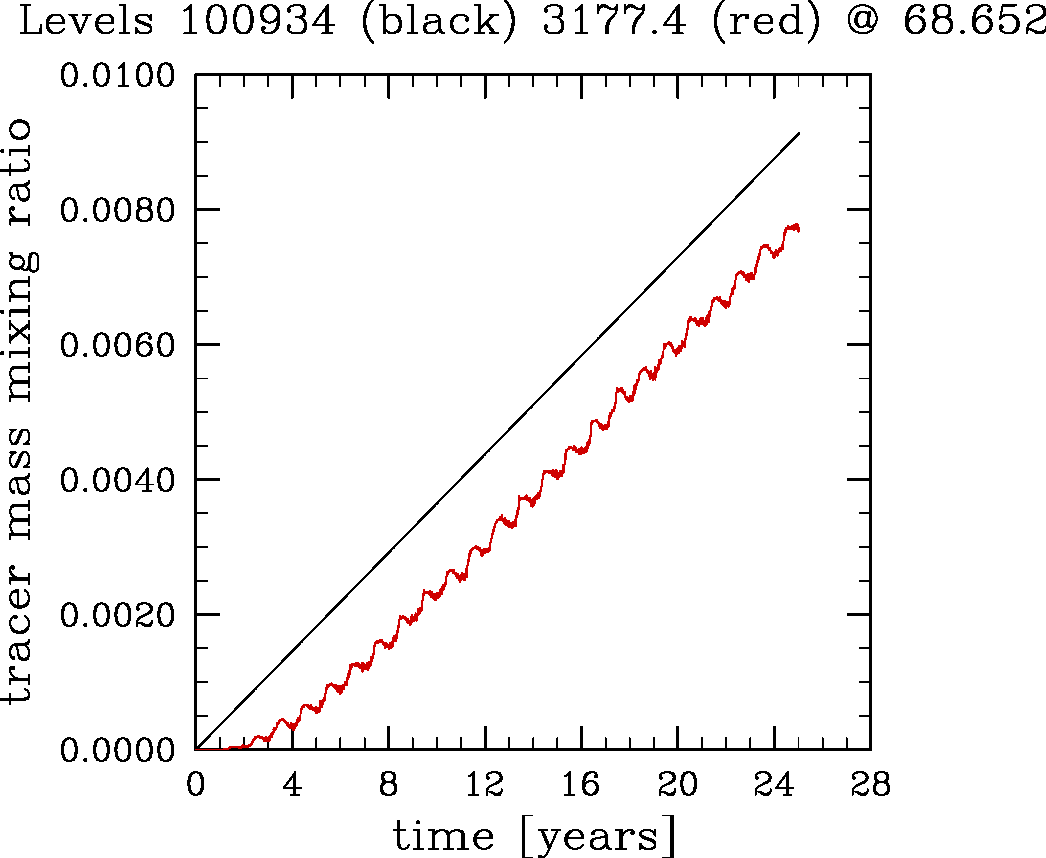
\includegraphics[width=12cm]{aoa_tracer_sample.pdf}
\igcrtwzeonfozefizenirjs{width=12cm}{aoa_tracer_sample.pdf}
\caption{The concentration of a passive tracer over time is shown at
  two different levels at $\approx 69^{\circ}$N in a model simulation
  performed with an early version of the ECHAM6 GCM under stationary
  present-day boundary conditions. The time lag between the
  concentrations can be used to derive the transport time of an air
  parcel from one grid point to the other and, thus, the age of
  air.}\label{fig_cr20140509rjs_aoa_tracer_sample} 
\end{figure}

Although the passive tracer is usually initialised at the surface, the
tropical tropopause is commonly used as the reference point for the
age of a stratospheric air parcel. As tracers are distributed rapidly
within the troposphere, the reference point can simply be set to a
certain location close to the tropical tropopause by subtracting the
tracer concentration at the reference grid point from any grid point
above. Following \cite{manzini1999} we use the 110 hPa level at the
equator as the reference grid point to calculate the age of air. The
zonal-mean age of air, obtained from all grid points above this
reference level in the 50-year present-day time-slice simulation with
ECHAM6, is shown in
Figure~\ref{fig_cr20140509rjs_age_of_air_sample}. The depicted age of
air distribution reflects the transport of air parcels along the
residual circulation trajectories in a coherent way. 

\begin{figure}
\centering
%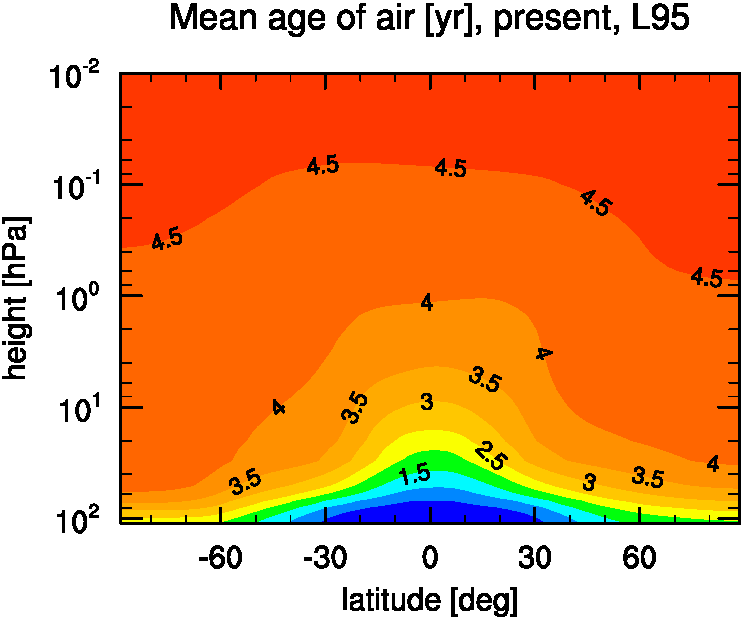
\includegraphics[width=12cm]{age_of_air_sample.pdf}
\igcrtwzeonfozefizenirjs{width=12cm}{age_of_air_sample.pdf}
\caption{The mean transit time of an air parcel originating from the
  tropical tropopause, i.e. the mean age of air, is shown. As in
  \cite{manzini1999}, the reference grid box is the 110 hPa level at
  the equator. The data represents the mean over the 50-year
  present-day time-slice simulation performed with the ECHAM6 GCM
  using 95 levels.}\label{fig_cr20140509rjs_age_of_air_sample} 
\end{figure}

Following \cite{hall1994} we derive the age spectrum of an air parcel
from a simulation of the spatio--temporal distribution of a tracer
that was injected into the atmosphere in a pulse. 
For a single time step the
mixing ratio of a passive tracer is set to 1 at every grid point
between -5 and +5 degrees latitude in the lowermost model
level. Before and after this time step the mixing ratio is forced to
zero at the same grid points. In this way the tracer concentration in
the injection grid points is as close as possible to Dirac's delta
distribution. Consequently, 
$n(P_0,t-t')$ can be substituted by $\delta(t-t_0)$ in
Equation~(\ref{eq_cr20140509rjs_green}) approximately,
leading to $G(P,P_0,t-t_0)=n(P,t)$. This shows that the age spectrum
$G(P,P_0,t-t_0)$ at any grid point $P$ is given by the tracer
concentration in that grid point. A certain amount of this tracer
pulse escapes the injection grid points between the injection and the
following time step. In order to normalise the age spectrum it is
divided by the total abundance of the tracer species left in the model
at the time step, at which the age spectrum is read out. To account
for seasonal differences in transport, one tracer pulse is injected on
January 1 and another one on July 1. Every 12 years tracer
concentrations are being reset, and a new pulse is injected. By
building the mean age spectrum of several tracer pulses, effects
originating from possible special atmospheric states can be
reduced. Figure~\ref{fig_cr20140509rjs_aoa_spectrum_sample} shows the
zonal-mean age spectrum of an air parcel at one grid point in the
high-latitude lower stratosphere in the 50-year present-day time-slice
simulation with ECHAM6, calculated by using the method described
above. The age spectrum peaks at roughly 2.5 years, while the long
tail of the spectrum reflects recirculated air parcels with an age of
up to the maximum age of 12 years (as tracer concentrations are being
reset after 12 years, see above). 

\begin{figure}
\centering
%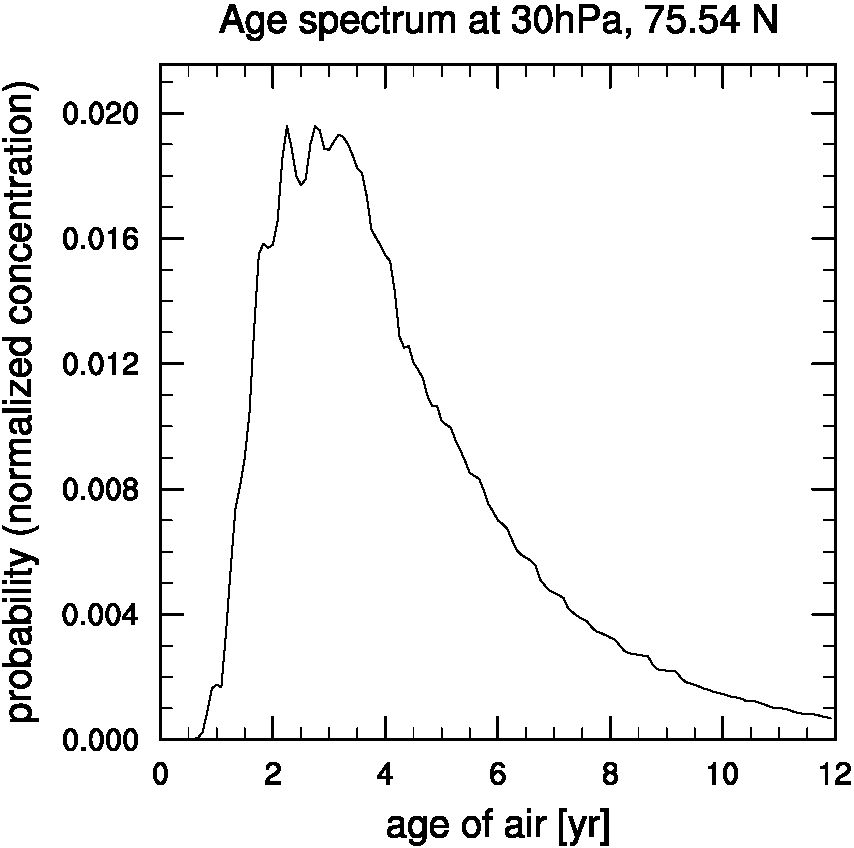
\includegraphics[width=12cm]{aoa_spectrum_sample.pdf}
\igcrtwzeonfozefizenirjs{width=12cm}{aoa_spectrum_sample.pdf}
\caption{The age spectrum of an air parcel located at 30 hPa and
  $75^{\circ}$N is shown. The data was derived from the 50-year
  present-day time-slice simulation performed with the ECHAM6 GCM
  using 95 levels.}\label{fig_cr20140509rjs_aoa_spectrum_sample} 
\end{figure}

\subsection{Implementation}

The age--of--air submodel consists of three passive tracers, one for
the mean age of air {\tt mean\_age}, and two that are used to
calculate the age spectra for winter and summer ({\tt spec\_winter},
{\tt spec\_summer}). 

\begin{description}
\item[{\tt init\_aoa}:] The age of air submodel consists of the 
subprograms {\tt init\_aoa},
{\tt bcond\_aoa}, {\tt get\_pointer2trac}, {\tt tracer\_reset}, and
{\tt tf\_reset} that are all collected in the module {\tt
  mo\_aoa.f90}. \newline
The subroutine {\tt init\_aoa} reads the namelist {\tt aoactl} 
from the file {\tt namelist.echam}, creates the tracers {\tt mean\_age},
{\tt spec\_winter}, and {\tt spec\_summer}, and sets the 
2--dimensional emission mask
{\tt emissions\_mask} to $1.0$ for each grid box where the tracers are
emitted, to $0$ where no emission takes place. Furthermore, the index
of the model level at which the emissions are injected into the
atmosphere is determined.
 
\item[{\tt bcond\_aoa}:]
Adds the emission rate to the tracer tendencies of {\tt mean\_age}, 
{\tt spec\_winter}, and {\tt spec\_summer}, respectively. The emission
rates are added only where {\tt emission\_mask} is larger than zero and
only if the model time lies in the appropriate time interval.
In the case of age--of--air tracers, the emission region is small 
compared to the globe and a {\tt where}--statement may be faster than 
a multiplication of the emission rate by {\tt emission\_mask}.

\item[{\tt get\_pointer2trac}:] This subroutine provides pointers to the 
3--dimensional fields hosting the mass mixing ratios of the tracers
{\tt mean\_age}, {\tt spec\_winter}, and {\tt spec\_summer} at
time step $t$ and $t-\Delta t$, respectively.

\item[{\tt tracer\_reset}, {\tt tf\_reset}:] 
The winter and summer tracer {\tt spec\_winter} and {\tt spec\_summer} 
have to be reset to zero after certain time intervals given
by the namelist in order to have good statistics in the determination
of the age spectrum. The program allows for a maximum number of
four re--initializations of these tracers. The variables
{\tt xt}, {\tt xtm1}, and {\tt pxtte} are reset in {\tt tracer\_reset},
the variable {\tt xtf} is reset in the {\tt tr\_reset}. The latter
variable occurs in the time filter and has to be reset also in order
to achive a complete re--initialization of the tracer.
\end{description}

\subsection{Usage}
\subsubsection{Namelist}
The age--of--air tracers controlled by the namelist {\tt aoactl}. 
It contains the following variables:

\setlength{\LTcapwidth}{\textwidth}
\setlength{\LTleft}{0pt}\setlength{\LTright}{0pt}

\begin{longtable}{l@{\extracolsep\fill}lp{6cm}l}\hline\hline
\caption[Namelist aoactl]{Namelist {\tt aoactl}}\\\hline
\label{tab_cr20140509_aoactl}
\endfirsthead
\caption[]{aoactl --- continued}\\\hline
\endhead
\hline\multicolumn{2}{r}{\slshape table continued on next page}\\
\endfoot
\hline %\multicolumn{2}{r}{end of table}
\endlastfoot
Variable & Type & Explanation & Default\\\hline
{\tt conc\_increase} & double prec. & increase of {\tt mean\_age} tracer
in mass mixing ration per day. The mass mixing ratio in the region where
${\tt emission\_mask} > 0$ is ${\tt conc\_increase}\times t$ after time $t$. 
& {\tt 1.0e-6\_dp}\\
{\tt dt\_start\_emi\_summer\_1} & integer(6) & year, month, day, hour, minute, 
second of first time that the emission of the tracer {\tt spec\_summer} starts.
The emission lasts one time step only. The date should be in summer. 
& {\tt 1978,1,2,0,0,0}\\
{\tt dt\_start\_emi\_summer\_2} & integer(6) & year, month, day, hour, minute, 
second of second time that the emission of the tracer 
{\tt spec\_summer} starts.
The emission lasts one time step only. The date should be in summer and about 
12~years after {\tt dt\_start\_emi\_summer\_1}. & {\tt 1990,1,2,0,0,0}\\
{\tt dt\_start\_emi\_summer\_3} & integer(6) & year, month, day, hour, minute, 
second of third time that the emission of the tracer 
{\tt spec\_summer} starts.
The emission lasts one time step only. The date should be in summer and about 
12~years after {\tt dt\_start\_emi\_summer\_2}. & {\tt 2002,1,2,0,0,0}\\
{\tt dt\_start\_emi\_summer\_4} & integer(6) & year, month, day, hour, minute, 
second of second time that the emission of the tracer 
{\tt spec\_summer} starts.
The emission lasts one time step only. The date should be in summer and about 
12~years after {\tt dt\_start\_emi\_summer\_3}. & {\tt 2014,1,2,0,0,0}\\
{\tt dt\_start\_emi\_winter\_1} & integer(6) & year, month, day, hour, minute, 
second of first time that the emission of the tracer {\tt spec\_winter} starts.
The emission lasts one time step only. The date should be in winter. 
& {\tt 1978,1,2,0,0,0}\\
{\tt dt\_start\_emi\_winter\_2} & integer(6) & year, month, day, hour, minute, 
second of second time that the emission of the tracer 
{\tt spec\_winter} starts.
The emission lasts one time step only. The date should be in winter and about 
12~years after {\tt dt\_start\_emi\_winter\_1}. & {\tt 1990,1,2,0,0,0}\\
{\tt dt\_start\_emi\_winter\_3} & integer(6) & year, month, day, hour, minute, 
second of third time that the emission of the tracer 
{\tt spec\_winter} starts.
The emission lasts one time step only. The date should be in winter and about 
12~years after {\tt dt\_start\_emi\_winter\_2}. & {\tt 2002,1,2,0,0,0}\\
{\tt dt\_start\_emi\_winter\_4} & integer(6) & year, month, day, hour, minute, 
second of second time that the emission of the tracer 
{\tt spec\_winter} starts.
The emission lasts one time step only. The date should be in winter and about 
12~years after {\tt dt\_start\_emi\_winter\_3}. & {\tt 2014,1,2,0,0,0}\\
{\tt emission\_lat\_n} & double prec. & latitude of the northern boundary of the emission 
region in degrees north& $5^\circ$ \\
{\tt emission\_lat\_s} & double prec. & latitude of the southern boundary of the emission 
region in degrees north& $-5^\circ$ \\
{\tt emission\_plev} & double prec. & Pressure level of emission in hPa. More 
precisely, the emission is injected in the model level with the
lowest pressure at the midpoint of which the
pressure at the lower boundary is larger than {\tt emission\_plev}. 
The pressure of the model levels are determined using a surface pressure
of $101325\,{\rm Pa}$. & $1013.25\,{\rm hPa}$\\
\hline
\end{longtable}
 
\subsubsection{Postprocessing}
There are two ncl--scripts provided at \newline
{\tt https://svn.zmaw.de/svn/diagnostics/trunk/diagnostics/echam/}
\newline
that create 
graphical output of the age of air calculated from the tracer output 
of the age--of--air submodel. The {\tt contour\_age.ncl} script 
creates a contour plot with the mean age of air from the {\tt mean\_age}
tracer, {\tt aoa\_spectrum.ncl} calculates the age spectrum of air at
a certain model level and latitude.

\paragraph{contour\_age.ncl:} This script requires yearly files with 
monthly means, but it can calculate the zonal mean by itself. There are 
lines at the beginning of the ncl--script that have to be adjusted to 
the actual experiment.
\setlength{\LTcapwidth}{\textwidth}
\setlength{\LTleft}{0pt}\setlength{\LTright}{0pt}
\begin{longtable}{l@{\extracolsep\fill}p{9cm}}\hline\hline
\caption[Variables of contour\_age.ncl]
{Variables of {\tt contour\_age.ncl}}\\\hline
\label{tab_cr20140509_contourage}
\endfirsthead
\caption[]{contour\_age --- continued}\\\hline
\endhead
\hline\multicolumn{2}{r}{\slshape table continued on next page}\\
\endfoot
\hline %\multicolumn{2}{r}{end of table}
\endlastfoot
\hline
Variable & Explanation \\\hline
{\tt cdo\_cmd} & cdo--command that will be executed before the mean
age is calculated, e.g. {\tt ``zonmean''} for the calculation of zonal
mean values, or {\tt ``zonmean -monmean''} to calculate monthly means
and zonal means.\\
{\tt climean} & period of time over which the monthly means are averaged,
e.g. {``YEAR''}, {``DJF''}, or {``JJA''}.\\
{\tt datdir} & path of input files\\
{\tt dstring} & Plot title\\
{\tt expm} & infix of input files describing the experiment, e.g. 
{\tt ``DEV0107''}\\
{\tt emission\_start}& start year of emissions\\
{\tt first\_year} & first year from which the global tracer increase
can be considered to be linear.\\
{\tt fname\_suffix} & suffix of \echam{} input files. In most cases either 
{\tt ``tracer''} or {\tt ``tracerm''}\\
{\tt last\_year} & last year that will be used in the age--of--air 
calculation\\
{\tt lat\_idx\_n} & index of northern latitude up to which the age
of air is calculated. It has to be counted from the equator. E.g. 46
in the case of a horizontal resolution T63.\\
{\tt lat\_idx\_s} & index of southern latitude up to which the age of air is
calculated. It has to be counted from the equator, E.g. 47 in the 
case of a horizontal resolution T63.\\
{\tt proj} & will be a part of the ourput filename, e.g. {\tt ``SHARP''}\\
{\tt reflevel} & pressure in hPa at which the age of air is 
defined to be zero. Usually, {\tt relevel=11000}, i.e.~ the age 
of air is assumed to be zero at $110\,{\rm hPa}$. \\
{\tt wks\_type} & format of graphics output, e.g. {\tt ``eps''}\\
\end{longtable}

\paragraph{aoa\_spectrum.ncl:} This script requires yearly files with 
monthly means of the pulsed tracers {\tt spec\_winter} and 
{\tt spec\_summer}. There are 
lines at the beginning of the ncl--script that have to be adjusted to 
the actual experiment.
\setlength{\LTcapwidth}{\textwidth}
\setlength{\LTleft}{0pt}\setlength{\LTright}{0pt}
\begin{longtable}{l@{\extracolsep\fill}p{9cm}}\hline\hline
\caption[Variables of aoa\_spectrum.ncl]
{Variables of {\tt aoa\_spectrum.ncl}}\\\hline
\label{tab_cr20140509_aoaspectrum}
\endfirsthead
\caption[]{aoa\_spectrum --- continued}\\\hline
\endhead
\hline\multicolumn{2}{r}{\slshape table continued on next page}\\
\endfoot
\hline %\multicolumn{2}{r}{end of table}
\endlastfoot
\hline
Variable & Explanation \\\hline
{\tt datdir} & path of input files\\
{\tt cdo\_cmd} & cdo--command that will be executed before the mean
age is calculated, e.g. {\tt ``zonmean''} for the calculation of zonal
mean values, or {\tt ``zonmean -monmean''} to calculate monthly means
and zonal means.\\
{\tt emission\_years} & time interval between emission pulses in years\\
{\tt expm} & infix of input files describing the experiment, e.g. 
{\tt ``DEV0107''}\\
{\tt first\_emissions} & year of first emission pulse\\
{\tt fname\_suffix} & suffix of \echam{} input files. In most cases either 
{\tt ``tracer''} or {\tt ``tracerm''}\\
{\tt latidx} & index of latitude at which age spectrum is to be calculated\\
{\tt levidx} & index of level at which age spectrum is to be calculated\\
{\tt no\_of\_trac} & total number of emission pulses\\
{\tt proj} & will be a part of the ourput filename, e.g. {\tt ``SHARP''}\\
{\tt wks\_type} & format of graphics output, e.g. {\tt ``eps''}\\
\hline
\end{longtable}
%\begin{lstlisting}
%code
%\end{lstlisting}



\clearpage\newpage

\section[cr2014\_07\_14\_rjs: Radiative convective equilibrium]{cr2014\_07\_14\_rjs:
  Simulation of radiative--convective equilibrium using \echam}\label{cr20140715rjs}

\subsection{Introduction}

The radiative--convective equilibrium (RCE) offers a possibility
to improve our fundamental understanding of processes in the
atmosphere and their impact on climate change
(e.g.~\cite{man641}). The idea behind this simplified modeling
of the atmosphere 
is that the basic 
atmospheric structure, especially in the tropics, is determined by the
balance between cooling of the atmosphere through radiative processes
and a commensurate heating through convection, mainly by the net
release of latent heat through precipitation. 

The RCE has been investigated in models of different complexity,
ranging from simple energy balance, 1--dimensional column models to
high resolution LES simulations. The RCE is also implemented into the 
general circulation model \echam{} by creating a model configuration,
where the resulting climate is given merely through the balance of
radiative processes and convection. Columns can interact with each
other and thus create a mean three--dimensional circulation which
develops interactively, although it is very different from the general
circulation we know from the real Earth. E.g., the RCE results in slowly moving
convective clusters of sometimes continental extension (\cite{pop131}).  

To inhibit net energy transport from the tropics to the poles,
homogeneous boundary conditions are specified, where every gridpoint
of the sphere receives the same incoming solar radiation
(e.g.~$340\,{\rm W/m^2}$). A diurnal
cycle may be switched on but is kept exactly the same for each column
representing a pulsating light source shining from all directions
equally. The Earth's rotation velocity is set to zero. In the standard
RCE configuration, land--sea contrasts are removed by specifiying an
underlying mixed--layer ocean with a constant ocean albedo, but can
easily be included in idealized form for land--sea contrast
studies~(\cite{bec14x}). Besides the modifications mentioned 
above and technical details listed below, the results of the
ECHAM--RCE 
well resemble the tropics of a control simulation with the full
\echam{} model in the mean
state~\cite{pop131}.
However, this model version has not been tested
for possible equilibria dependence on the initial boundary conditions
yet, nor for complete isotropy of variables expected from the
homogeneous boundary conditions. 

\subsection{Namelist settings for radiative--convective equilibrium}

The simulation of the radiative--convective equilibrium needs some
special namelist settings in order to switch off the diurnal cycle for
example. Table~\ref{tab_cr20140715_rcenamelist} gives an
overview of the necessary settings.

\setlength{\LTcapwidth}{\textwidth}
\setlength{\LTleft}{0pt}\setlength{\LTright}{0pt}

\begin{longtable}{l@{\extracolsep\fill}p{6.0cm}p{2.5cm}}\hline\hline
\caption[RCE namelist]{Namelist setting for radiative--convective
  equilibrium simulations with \echam}\\\hline
\label{tab_cr20140715_rcenamelist}
\endfirsthead
\caption[]{RCE namelist --- continued}\\\hline
\endhead
\hline\multicolumn{3}{r}{\slshape table continued on next page}\\
\endfoot
\hline %\multicolumn{2}{r}{end of table}
\endlastfoot
\multicolumn{1}{c}{Variable} & \multicolumn{1}{c}{Explanation} & \multicolumn{1}{c}{default} \\\hline
\multicolumn{3}{c}{{\tt runctl} namelist}\\\hline
$ {\tt earth\_angular\_velocity} = {\tt 0.0}$ &  switch off Coriolis force: no rotation &
{\tt 7.29212e-5} \\
${\tt lrce} = {\tt .true.} $ & turn on radiative--convective equilibrium mode:\newline
                                same zenith angle at all grid points
                                with either a perpetual day or (${\tt
                                  ldiur}={\tt .true.}$) a diurnal
                                cycle that is equal for all grid
                                points (the irradiation is dimmed and
                                brightened independently of the
                                geographic position).\newline  
                                use constant ocean surface albedo (0.07)\newline
                                ignore dynamical planetary boundary
                                layer height in
                      planetary boundary layer calculation. & {\tt .false.}\\
${\tt ly360} = {\tt .true.}$ & use a 360 days calendar (this is not
a prerequisite for an RCE simulation) & {\tt
  .false.}\\
${\tt l\_orbvsop87}  = {\tt .false.}$ &  use PCMDI (AMIP) orbit that
does not change with time and corresponds to a Kepler orbit. & {\tt
  .true.}\\
\hline
\multicolumn{3}{c}{{\tt radctl} namelist}\\\hline
$ {\tt cecc}  = {\tt 0.0}$ &  eccentricity of Kepler orbit is set to
zero meaning that the orbit is circular & {\tt 0.016715} \\
$ {\tt cobld} = {\tt 0.0}$ & obliquity in degrees is set to zero &
{\tt 23.441} \\ 
$ {\tt iaero} = {\tt 0}  $ & simulate an aerosol free atmosphere &
{\tt 2} \\
$ {\tt isolrad} = {\tt 4\,{\rm or}\,5}$ & solar irradiation\newline
${\tt isolrad} = {\tt 4}$: solar irradiation for RCE including a
diurnal cycle. In this case, {\tt ldiur} must be set to {\tt .true.}\newline
${\tt isolrad} = {\tt 5}$: time constant solar irradiation for RCE. In
this case, {\tt ldiur} must be set to {\tt .false.}& {\tt 3}\\
$ {\tt icfc}    = {\tt 0}$ & switch off all effects of
chlorofluorocarbons &  {\tt 2} \\ 
\hline
\end{longtable}

\subsection{Initial and boundary conditions}

The initial and boundary conditions are different from the usual model
set--up since they are isotropic except for the initial conditions into
which a small perturbation of the isotropy is introduced.

The initial and boundary conditions can be generated in various
resolutions from initial and boundary condition files that exist
already. The script {\tt create\_initial\_files\_rce\_aqua.sh} is
provided at {\tt /pool/data/ECHAM6/input/r0004/rce/bin}. In order to
change the resolution, you have to modify the values of the variables
{\tt RES}, {\tt ILEV}, {\tt OCERES} according to the desired spectral
resolution, vertical levels, and ocean resolution, respectively. In
that case, initial and boundary condition files of standard \echam{}
have to exist in the new resolution {\tt RES}, {\tt ILEV}, {\tt
  OCERES} in {\tt /pool/data/ECHAM6/input/r0001}. The following
tables~\ref{tab_cr20140715_janspec}--\ref{tab_cr20140715_surf} give an
overview of the values of the variables modified for
radiative--convective equilibrium simulations with \echam.

\setlength{\LTcapwidth}{\textwidth}
\setlength{\LTleft}{0pt}\setlength{\LTright}{0pt}

\begin{longtable}{l@{\extracolsep\fill}p{11cm}}\hline\hline
\caption[Spectral initial data for RCE]{Spectral initial data in {\tt
    \{RES\}\{LEV\}\_jan\_spec\_rce.nc} for radiative--convective
  equilibrium simulations}\\\hline
\label{tab_cr20140715_janspec}
\endfirsthead
\caption[]{Spectral initial data for RCE --- continued}\\\hline
\endhead
\hline\multicolumn{2}{r}{\slshape table continued on next page}\\
\endfoot
\hline %\multicolumn{2}{r}{end of table}
\endlastfoot
Variable  & Description \\\hline
${\tt SVO} = 10^{-8}{\rm 1/s}$ & vorticity of the wind field, is
transformed to spectral space in the file\\
${\tt SD} = 10^{-8}{\rm 1/s}$ & divergence of the wind
field, is transformed to spectral space in the file\\
${\tt STP} = (300 {\rm K},11.5261)$ & temperature is set to $300
\rm{K}$ at all model levels globally and the logarithm of the surface
pressure $\ln(p_{\rm surf}/(1 {\rm Pa}))$. Both are transformed to
spectral space in the file and stored in the variable {\tt STP}, the
pressure is stored in the ``level'' ${\tt nlev} + 1$. \\
${\tt Q} = 10^{-8}$ & specific humidity stored in grid point space.\\\hline  
\hline
\end{longtable}

The vorticity and divergence of the wind field are set to a small
value in order to initiate dynamics in the atmosphere. Finally, this leads to
spatial inhomogeneities and triggers 
regional dynamics. 

The surface variables collected in {\tt
  \{RES\}\{OCR\}\_jan\_surf\_rce.nc} are mostly set to zero with only
a few exceptions. Table~\ref{tab_cr20140715_jansurf} lists the
respective variables.

\setlength{\LTcapwidth}{\textwidth}
\setlength{\LTleft}{0pt}\setlength{\LTright}{0pt}

\begin{longtable}{l@{\extracolsep\fill}p{9cm}}\hline\hline
\caption[Surface initial data for RCE]{Surface (initial) data in {\tt 
  \{RES\}\{OCR\}\_jan\_surf\_rce.nc} for radiative--convective
  equilibrium simulations}\\\hline
\label{tab_cr20140715_jansurf}
\endfirsthead
\caption[]{Surface initial data for RCE --- continued}\\\hline
\endhead
\hline\multicolumn{2}{r}{\slshape table continued on next page}\\
\endfoot
\hline %\multicolumn{2}{r}{end of table}
\endlastfoot
Variable  & Description \\\hline
${\tt SLM}=0$ & land--sea mask set to zero to indicate that there is ocean
everywhere \\
${\tt GEOSP}=0{\rm m^2/s^2}$ & The surface geopotential is set to zero (no
mountains)\\
${\tt WS}=0{\rm m}$ & soil wetness \\
${\tt SN}=0{\rm m}$ & snow depth \\
${\tt SLF}=0$ & fractional land--sea mask \\
${\tt AZ0}=0.001{\rm m}$ & surface roughness \\
${\tt ALB}=0.07$ & surface background albedo\\
${\tt FOREST}=0$ & vegetation type\\
${\tt WSMX}=10^{-13}{\rm m}$ & field capacity of soil\\
${\tt FAO}=0$ & FAO data set\\
${\tt GLAC}=0$ & glacier mask\\
${\tt ALAKE}=0$ & lake mask\\
${\tt OROMEA}=0{\rm m^2/s^2}$ & mean orography \\
${\tt OROSTD}=0{\rm m^2/s^2}$ & standard deviation of orography \\
${\tt OROSIG}=0^\circ$ & orographic slope\\
${\tt OROGAM}=0^\circ$ & orographic anisotropy\\
${\tt OROTHE}=0^\circ$ & orographic angle\\
${\tt OROPIC}=0{\rm m}$ & elevation of orographic peaks\\
${\tt OROVAL}=0{\rm m}$ & elevation of orographic valleys\\
\hline
\end{longtable}

The following files listed in Table~\ref{tab_cr20140715_surf} contain
variables related to boundary conditions 
at the surface:

\setlength{\LTcapwidth}{\textwidth}
\setlength{\LTleft}{0pt}\setlength{\LTright}{0pt}

\begin{longtable}{l@{\extracolsep\fill}lp{4cm}}\hline\hline
\caption[Surface initial data for RCE]{Surface boundary condition data
  for radiative--convective 
  equilibrium simulations}\\\hline
\label{tab_cr20140715_surf}
\endfirsthead
\caption[]{Surface boundary condition data for RCE --- continued}\\\hline
\endhead
\hline\multicolumn{3}{r}{\slshape table continued on next page}\\
\endfoot
\hline %\multicolumn{2}{r}{end of table}
\endlastfoot
Variable  & Description \\\hline
{\tt \{RES\}\_amip2sst\_rce.nc} & ${\tt sst}=300{\rm K}$ & sea surface temperature \\
{\tt \{RES\}\_amip2sic\_rce.nc} & ${\tt sic}=0\%$ & sea ice coverage\\
{\tt \{RES\}\_qflux\_rce.nc} & ${\tt aflux}=0$ & heat flux in the
ocean for simulations including mixed--layer ocean\\
\hline
\end{longtable}

As ozone profile, an equatorial column from an ozone file from the
AC\&C/SPARC ozone data base for CMIP5 for the year 1870 is taken and
stored in {\tt  \{RES\}\_ozone\_CMIP5\_rce.nc}.

For all other land--surface files, the usual \echam--files can be linked
since they do not have any influence on the results as long as the
planet has a pure ocean surface.


\end{appendix}
